% \documentclass{cumcmthesis}
\documentclass[withoutpreface,bwprint]{cumcmthesis} %去掉封面与编号页,电子版提交的时候使用。


\usepackage[noend]{algpseudocode}
\usepackage{algorithm}
\usepackage{algpseudocode}
\usepackage{amsmath}
\usepackage[framemethod=TikZ]{mdframed}
\usepackage{url}   % 网页链接
\usepackage{subcaption} % 子标题
\usepackage{threeparttable} 
\usepackage[table]{xcolor}


\title{基于机器学习与关联网络的古代玻璃成分分析}
\tihao{A}
\baominghao{4321}
\schoolname{XX大学}
\membera{ }
\memberb{ }
\memberc{ }
\supervisor{ }%辅导老师
\yearinput{2023}
\monthinput{9}
\dayinput{8}
\setcounter{tocdepth}{2}



\begin{document}

\maketitle

\begin{abstract}


古代玻璃的化学成分是鉴别其类别与产地的重要依据,然而风化作用会改变原始成分,为定量分析带来挑战。本文基于一批古代玻璃制品的化学成分数据,建立了一套多层次的数学模型,以解决风化影响下的玻璃分类、成分预测与内在关联分析问题。研究综合运用了统计检验、机器学习、智能优化算法与复杂网络理论,为通过化学成分数据理解古代玻璃制品提供了系统性的分析方案。


对于问题一,我们采用\textbf{卡方检验}分析了表面风化与玻璃类型、纹饰及颜色的关联性,确认了它们之间存在统计学关联。通过对比风化前后样本的化学成分分布,发现风化主要导致高钾玻璃中的氧化钾与铅钡玻璃中的氧化铅和氧化钡流失。为预测风化前的成分,本文引入\textbf{地球化学领域}的\textbf{质量平衡分析理论},构建了基于风化系数的预测模型,该模型在缺乏成对样本的情况下,能够有效恢复文物的原始化学成分。


对于问题二,为研究两大类玻璃的分类规律,我们分别构建了\textbf{线性与非线性支持向量机模型}。其中,非线性模型获得了97.41\%的交叉验证准确率,我们引入\textbf{博弈论中的SHAP值}对其进行解释,而线性模型的结果则直接验证了氧化铅与氧化钾是分类的核心指标。在亚类划分中,我们依据\textbf{变异系数}筛选特征,并结合\textbf{层次聚类}与\textbf{轮廓系数},确定铅钡玻璃存在两个亚类,高钾玻璃存在五个亚类。划分结果显示铅钡玻璃可分为高铅钡助熔剂型与高硅基质型,高钾玻璃的亚类则在多种成分上表现出不同特征。


对于问题三,我们构建了基于\textbf{改进遗传算法}优化的\textbf{支持向量机分类器IGA-SVM},以鉴别未知类别文物的所属类型。该模型通过智能化全局寻优确定最优超参数组合,避免了传统模型选择的局限性。应用此模型,我们完成了对全部未知样本的分类。为确保结果的可靠性,我们设计了基于\textbf{蒙特卡洛模拟}的数据扰动与基于\textbf{参数网格搜索}的模型扰动双重灵敏度分析,验证了分类结果对于数据测量误差和模型参数选择的高度稳健性。


对于问题四,为探寻不同类别玻璃配方的内在结构差异,我们构建了\textbf{化学成分关联网络}。为消除成分数据总和恒定带来的虚假相关,我们首先采用化学计量学中的\textbf{中心化对数比变换}对数据进行处理。随后利用\textbf{图套索算法}计算偏相关系数以构建网络,并应用\textbf{鲁汶算法}进行社群发现。网络分析结果表明,铅钡玻璃与高钾玻璃的化学成分关联结构存在显著不同,前者以二氧化硅和氧化铅为核心形成紧密社群,后者则结构较为分散,这些差异反映了两者在原料与烧制工艺上的区别。

\keywords{卡方检验 \quad 地球化学 \quad 质量平衡分析理论  \quad SHAP值 \quad 支持向量机 \quad 中心化对数比 \quad 图套索算法 \quad 鲁汶算法}


\end{abstract}


\section{问题背景}

古代丝绸之路不仅是商贸通道,也是文化与技术交流的重要桥梁,其中,玻璃制品是早期东西方物质文化交流的重要物证。早期玻璃制品由西亚和埃及地区传入,其技术与风格影响了中国本土的玻璃制造业。中国古代工匠在吸收外来技术的基础上,利用本土原料进行生产,制造出外观相似但化学成分体系相异的玻璃器物。这种成分上的差异为鉴别古代玻璃制品的产地与技术来源提供了客观依据。

玻璃的主要成分为二氧化硅 ($SiO_2$)。为降低其熔点,制造过程中需加入助熔剂。古代中西方采用的助熔剂体系不同,形成了成分各异的玻璃类别。例如,以草木灰为助熔剂的钾玻璃 ($K_2O$ 含量较高) 和以铅矿石为助熔剂的铅钡玻璃 ($PbO$、$BaO$ 含量较高),后者被普遍认为是古代中国独立发展的玻璃品种。然而,玻璃制品在长期埋藏过程中,其表面易与环境发生元素交换,导致化学成分发生改变,这一风化过程给准确的成分分析与类型鉴别带来了挑战。因此,需要建立一套系统的数据分析方法,以消除或减弱风化作用的干扰,准确识别玻璃文物的化学成分规律,并对其进行科学分类与鉴别。


\begin{figure}[htbp]
    \centering
    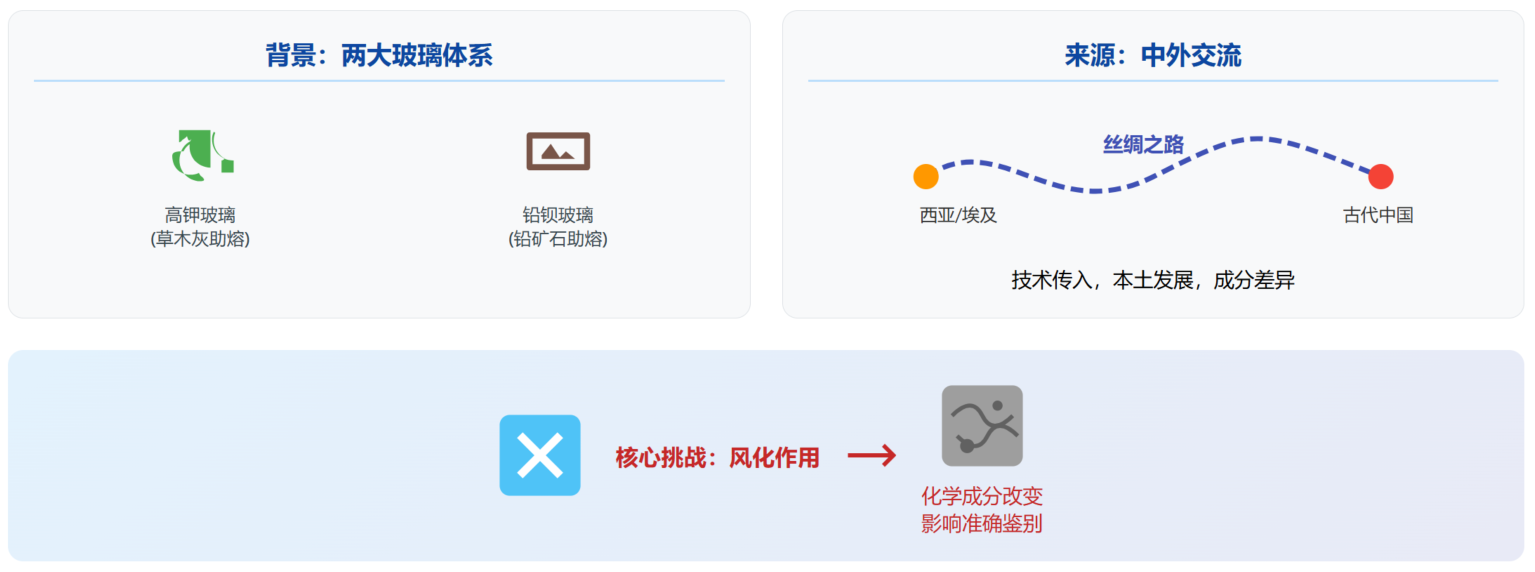
\includegraphics[width=\textwidth]{figs/1前置/问题背景.png}
    \caption{问题背景} 
    \label{fig:your_image_label} 
\end{figure}


\section{问题重述}

问题一:分析玻璃文物表面风化状态与其玻璃类型、纹饰和颜色等物理属性的统计关系。在此基础上,结合玻璃类型,研究表面风化对化学成分含量的影响规律,并建立数学模型,根据风化样品的化学成分数据,预测其风化前的成分含量。

问题二:根据已分类的高钾玻璃与铅钡玻璃的化学成分数据,建立有效的分类判据。进而,在每个大类中,选择合适的化学成分作为指标,对该类别进行亚类划分,并给出具体的划分方案。最后,对分类与划分结果的合理性及稳定性进行分析。

问题三:利用已建立的分类模型,对一批未知类别的玻璃文物样品的化学成分数据进行分析,鉴别其所属的玻璃类型。同时,需要对鉴别结果的敏感性进行评估,以考察分类结果的稳健程度。

问题四:针对高钾玻璃与铅钡玻璃两个类别,分别探究其内部各化学成分之间的关联关系。通过比较两个类别在化学成分关联模式上的异同,表现不同玻璃体系在原料构成与制造工艺上可能存在的差异。

\section{问题分析}

对于问题一,该问题包含两个递进的部分。第一部分要求分析风化状态与玻璃类型、纹饰、颜色等多个定性变量之间的关系,可采用列联表分析与卡方检验等统计方法,检验这些变量之间是否存在显著的相依性。第二部分旨在建立风化前后化学成分的映射关系。此过程可视为一个回归或预测问题,可以通过分析同一文物上风化点与未风化点的成分差异,建立多元回归模型,从而实现对风化前成分的定量估计。

对于问题二,其核心是分类与聚类任务。首先,区分高钾与铅钡玻璃是一个监督学习分类问题。由于类别标签已知,可利用逻辑回归、支持向量机或决策树等分类算法,建立基于化学成分的分类器。其次,在已确定的类别内部进行亚类划分,是一个无监督学习的聚类问题。因缺乏亚类的先验标签,可采用K-均值聚类或层次聚类等算法,依据关键化学成分的分布特征进行探索性划分。对结果的合理性分析可通过交叉验证评估分类器性能,通过轮廓系数等指标评价聚类效果;敏感性分析则可通过扰动数据来检验模型输出的稳定性。

对于问题三,该问题是问题二所建分类模型的直接应用。需要将表单三中未分类样本的化学成分数据输入已训练好的分类器,以获得其预测类别。其敏感性分析旨在评估分类决策的可靠性,可以通过计算样本点到分类边界的距离或在样本成分数据上施加微小扰动,观察分类结果是否发生改变,来衡量分类的稳健性。

对于问题四,该问题要求探究不同类别玻璃内部化学成分的相互关系。此分析可通过计算各类别样本的协方差矩阵或相关系数矩阵来实现。皮尔逊相关系数是衡量两个连续变量间线性关系强度的常用指标。通过为高钾和铅钡玻璃分别构建相关系数矩阵,并利用热力图等可视化手段,可以直观地展示不同类别玻璃内部各元素间的协同或拮抗关系,比较其模式差异,为探究其工艺与原料来源提供数据支持。


\section{数据预处理与分析}

为了后续模型的建立与求解,本文进行如下数据预处理,即数据清洗、数据量化等。具体机制如图\ref{fig:数据预处理机制}所示。

\begin{figure}[htbp]
	\centering
	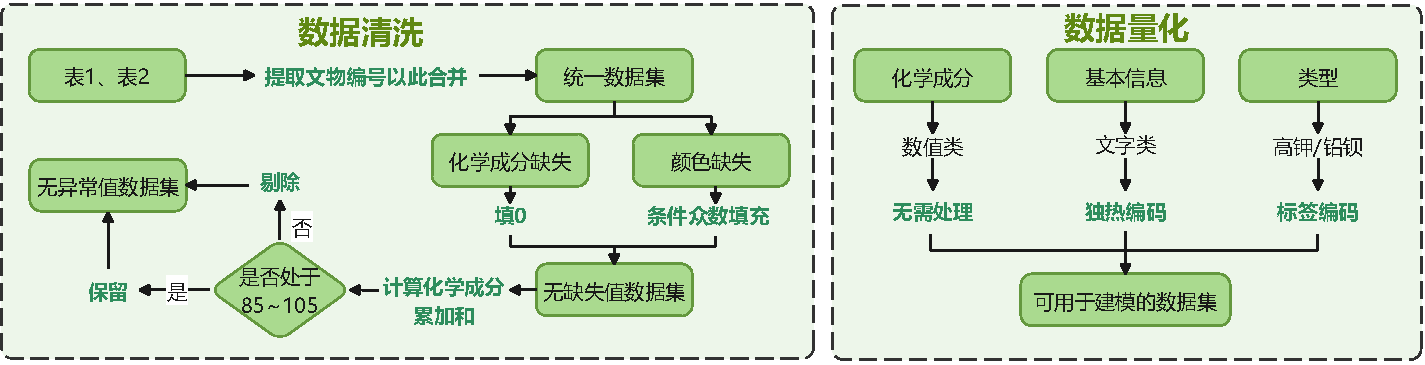
\includegraphics[width=\textwidth]{figs/2模型准备/数据预处理图.pdf}
	\caption{数据预处理机制}
	\label{fig:数据预处理机制}
\end{figure}

\subsection{数据清洗}

本文首先进行了数据清洗。题中给出的附件包含三个表单,表单1包含文物编号、纹饰、类型、颜色和表面风化情况,表单2则包含了文物采样点和化学成分比例。通过观察发现,表单2的“文物采样点”列前缀的数字部分与表单1的文物编号相对应,因此我们通过正则表达式提取出其数字部分,创建出“文物编号”列,并基于此将表单1内容合并进来,形成包含完整信息的数据集。

随后我们对数据集中各变量进行缺失值统计,发现颜色和化学成分比例存在显著的缺失问题。题目中提到表单2中化学成分比例若存在空白处表示未检测到该成分,因此我们将这些缺失值填充为0,处理前后的化学成分频数如图\ref{fig:缺失值填充}所示。

\begin{figure}[htbp]
	\centering
	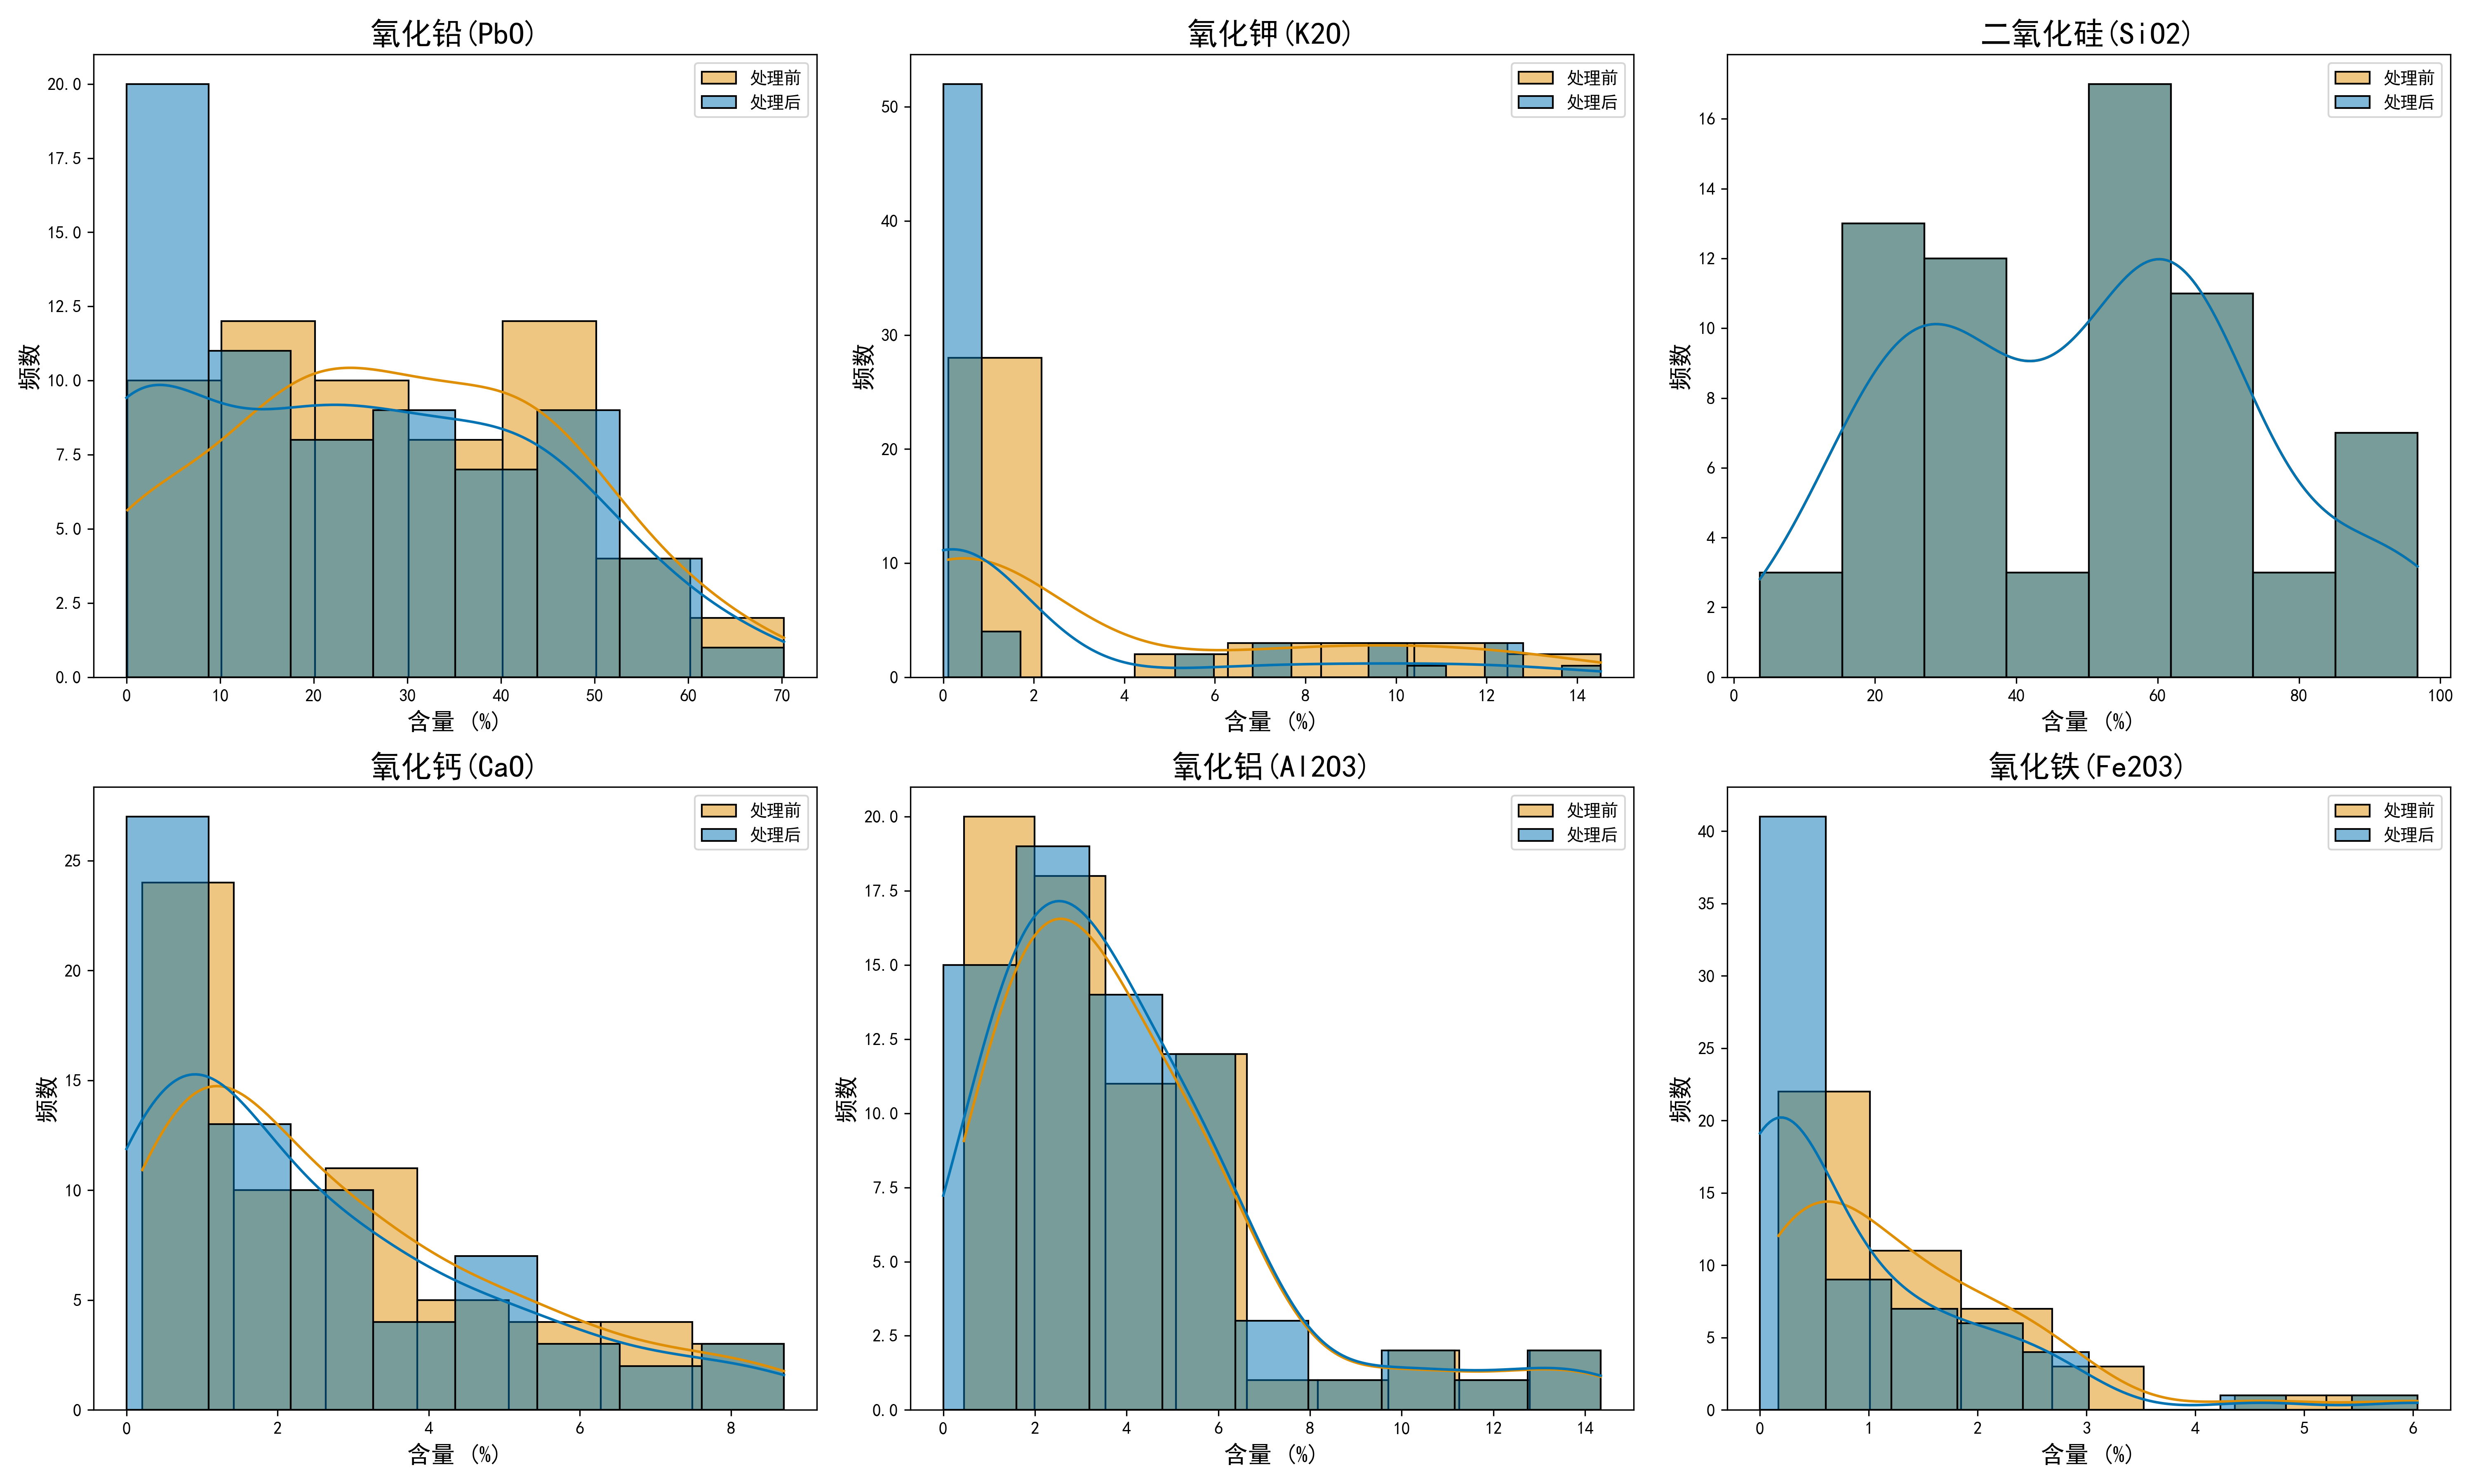
\includegraphics[width=0.8\textwidth]{figs/2模型准备/化学成分缺失值填充.png}
	\caption{化学成分缺失值填充}
	\label{fig:缺失值填充}
\end{figure}

而对于颜色缺失,我们首先想到通过全局众数填充,但是其误差可能较大,于是我们采用了一种条件众数填充法。具体而言,对于一个颜色信息缺失的样本,系统会自动寻找数据集中所有与该样本在类型、表面风化和纹饰上完全一致的其他样本,然后用这个小群体中出现次数最多的颜色来填充缺失值。其填充内容如图\ref{fig:颜色缺失值填充}所示。

\begin{table}[htbp]
	\centering
	\caption{按类型和纹饰划分的颜色众数及对应文物编号}
	\label{tab:颜色缺失值填充}
	\begin{tabular}{llll}
		\toprule
		\textbf{类型} & \textbf{纹饰} & \textbf{颜色众数} & \textbf{对应文物编号}                                        \\
		\midrule
		\rowcolor{gray!20}
		铅钡          & A           & 浅蓝            & \parbox[t]{6cm}{2, 19, 20, 23, 28, 29, 30, 42, 44, 45, \\ 46, 47, 48, 49, 50, 53} \\
		铅钡          & C           & 浅蓝            & \parbox[t]{6cm}{8, 11, 24, 25, 26, 31, 32, 33, 34, 35, \\ 36, 37, 38, 39, 40, 41, 43, 51, 52,  \\ 54,55, 56, 57, 58} \\
		\rowcolor{gray!20}
		高钾          & A           & 蓝绿            & 3, 4, 5, 6, 18, 21                                     \\
		高钾          & B           & 蓝绿            & 7, 9, 10, 12, 22, 27                                   \\
		\rowcolor{gray!20}
		高钾          & C           & 浅蓝            & 1, 13, 14, 15, 16, 17                                  \\
		\bottomrule
	\end{tabular}
\end{table}

针对各种化学成分比例,本题中将成分比例累加和介于85\%~105\%之间的数据视为有效数据,因此我们对其进行成分性异常值检测。我们计算每个样本所有化学成分的累加和,并筛选出总和介于85\%到105\%之间的数据作为有效样本,得到67条有效已分类样本、8条有效未分类样本以及2条异常样本,然后剔除异常样本。

最后我们检测了高钾玻璃和铅钡玻璃以及它们中风化和未风化的占比,如图\ref{fig:玻璃类型分布}所示:
\begin{figure}[htbp]
	\centering
	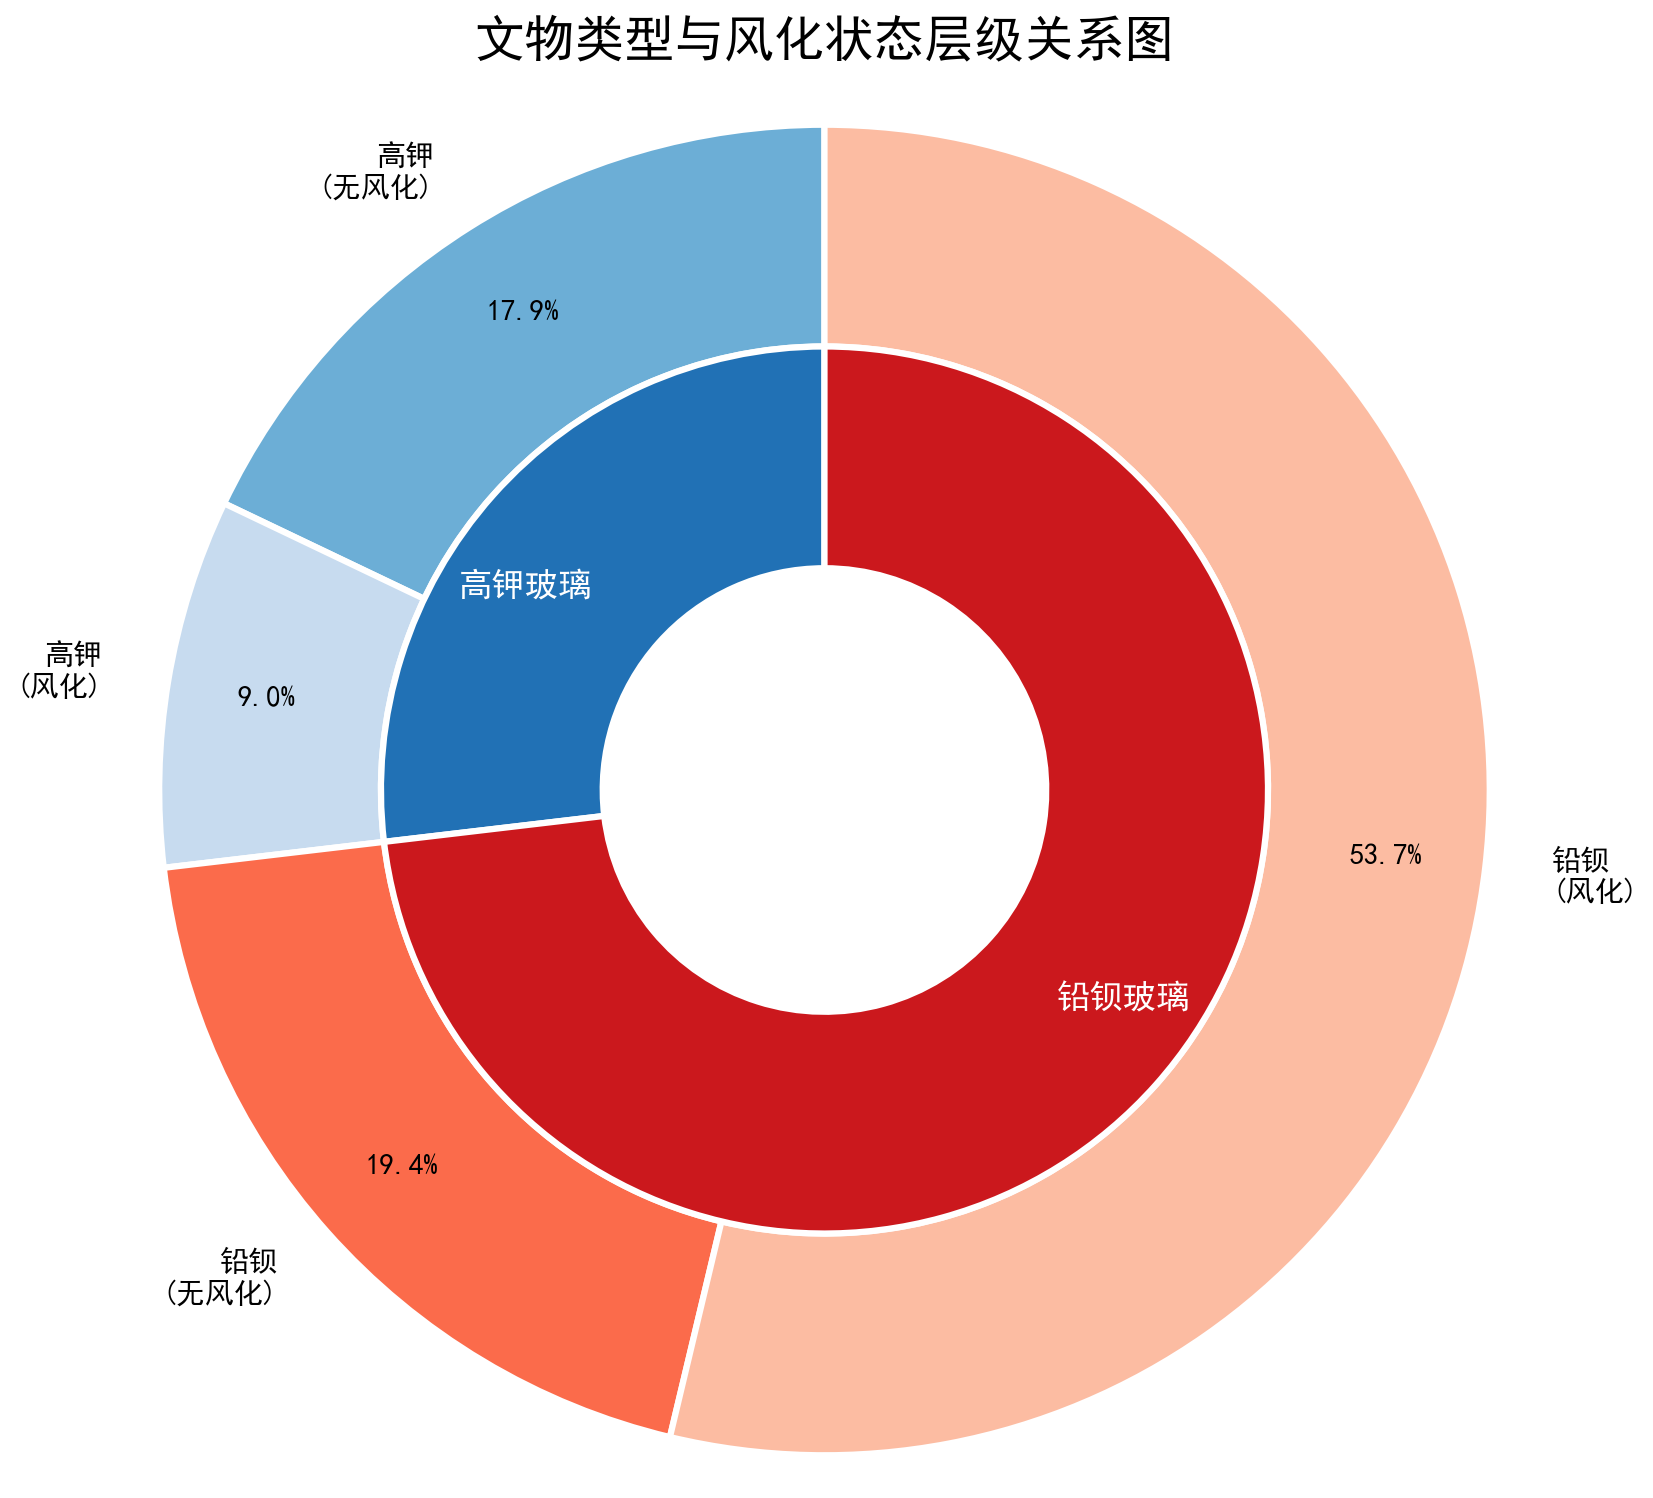
\includegraphics[width=0.5\textwidth]{figs/2模型准备/类型与风化嵌套饼图.png}
	\caption{类型与风化嵌套饼图}
	\label{fig:玻璃类型分布}
\end{figure}
从图中可以看出,类型、风化这两个核心分类变量的样本量均衡,故后续建模无需进行特殊的不平衡处理。

数据清洗的整体效果如图\ref{fig:数据清洗效果}所示。
\begin{figure}[htbp]
	\centering
	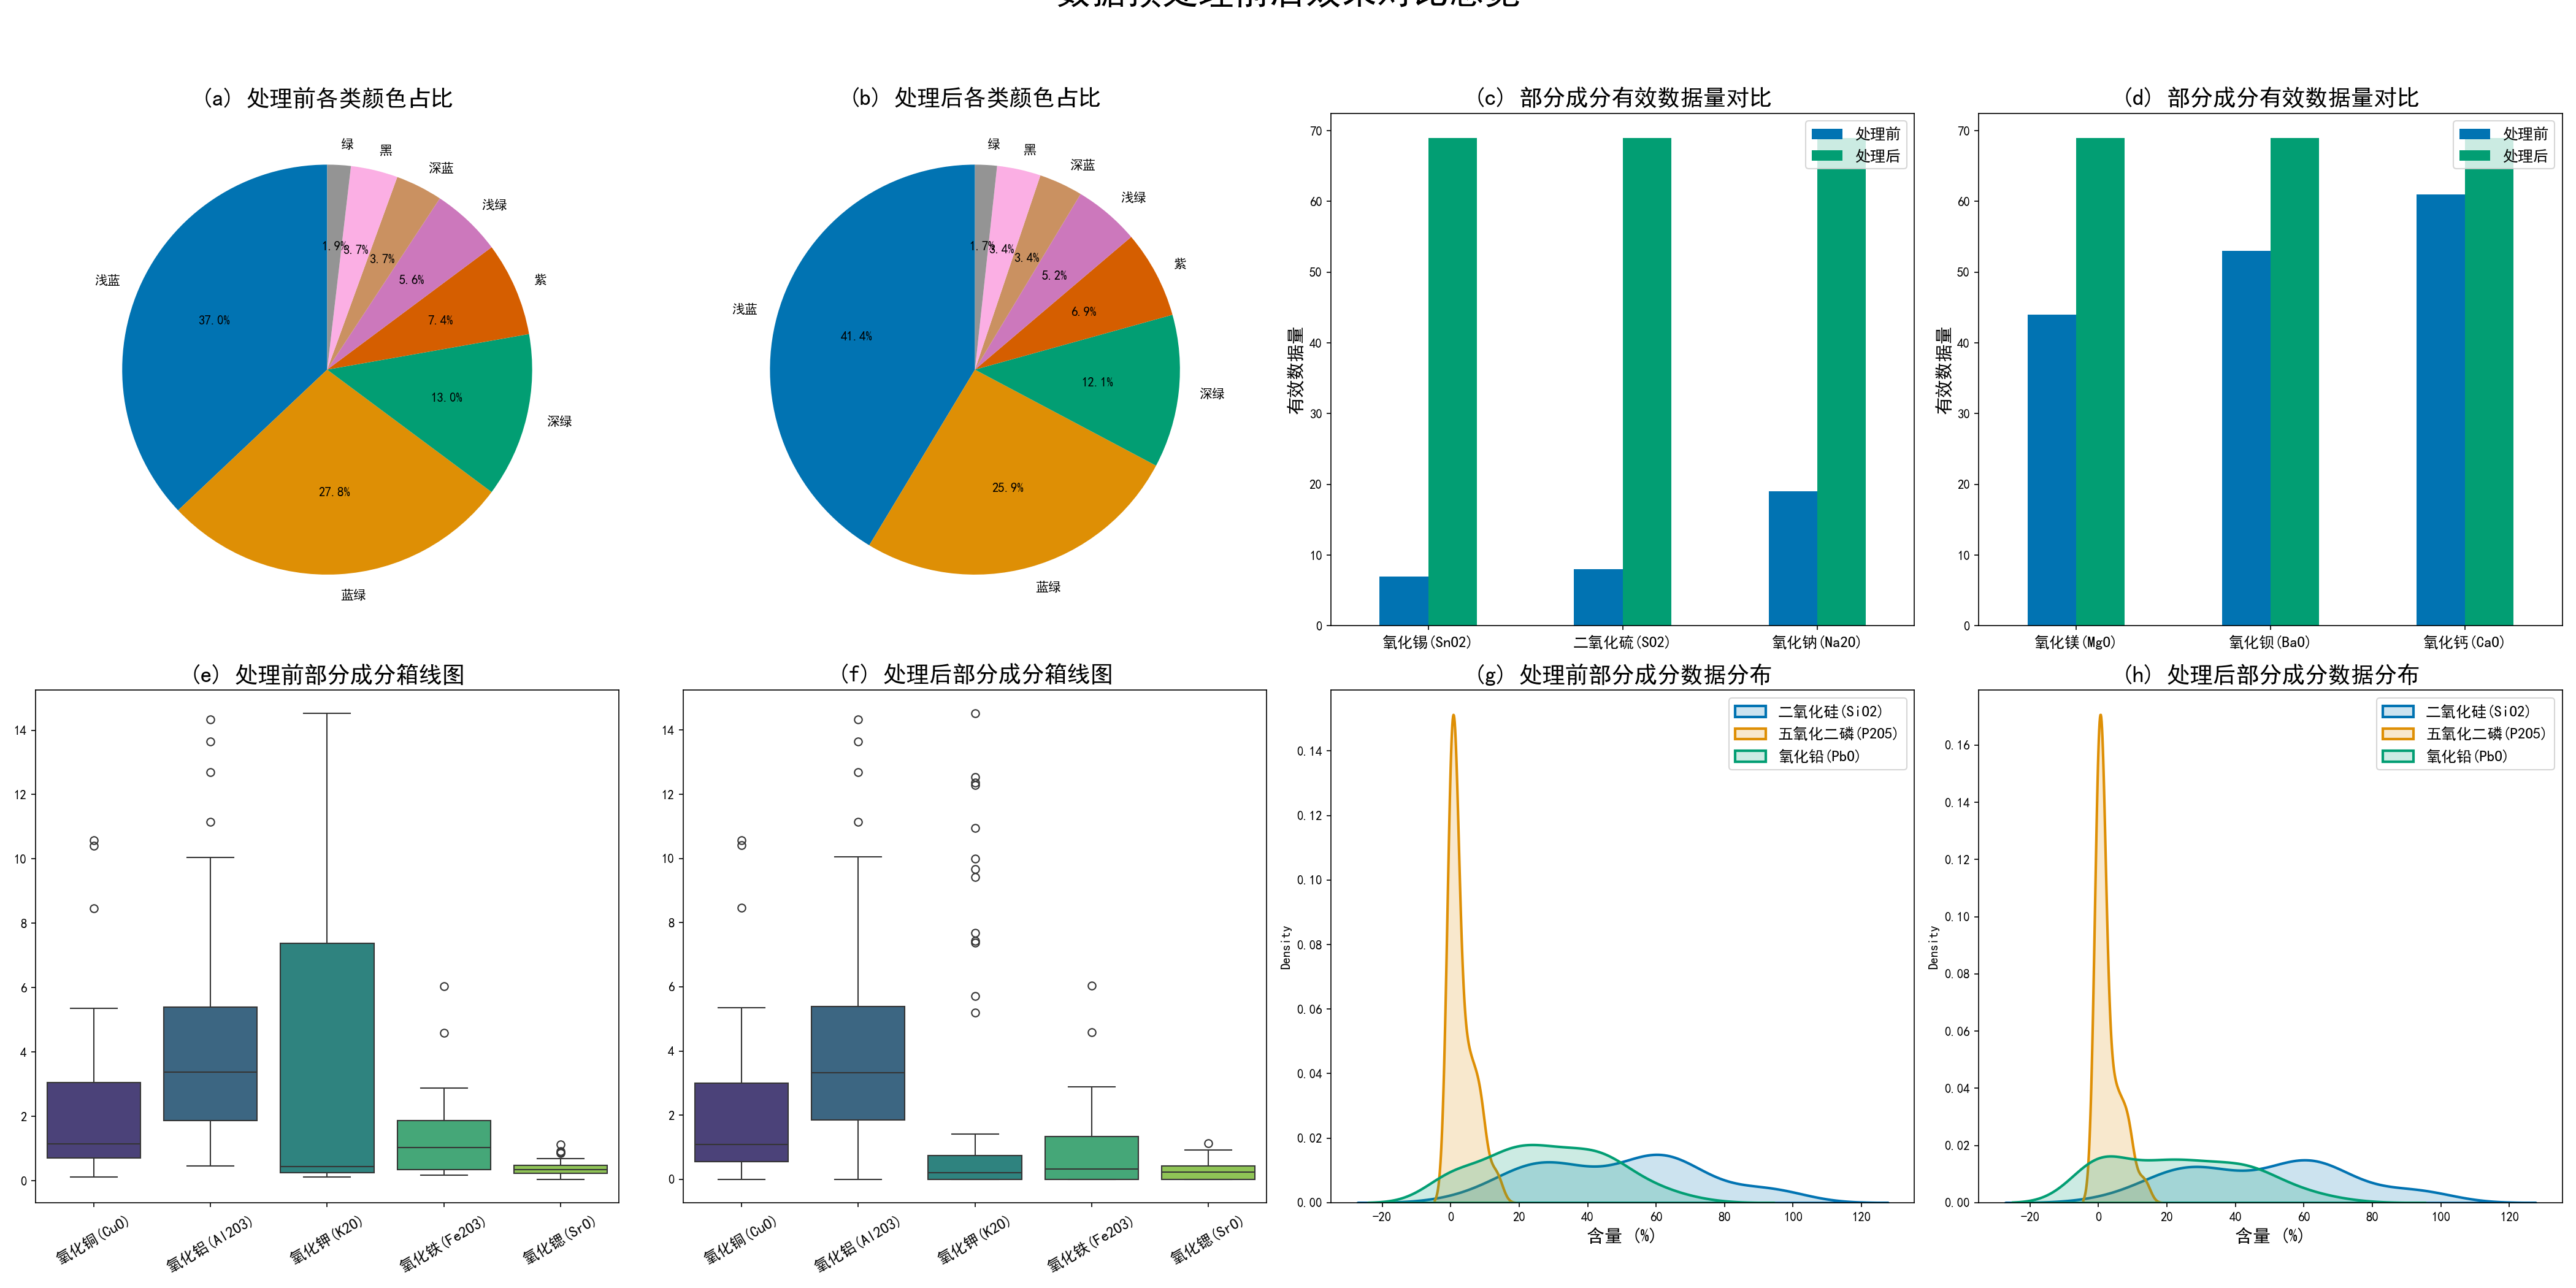
\includegraphics[width=\textwidth]{figs/2模型准备/预处理效果.png}
	\caption{数据清洗效果}
	\label{fig:数据清洗效果}
\end{figure}


\subsection{数据量化}

本文为了便于后续相关数学模型的建立与求解,增强可理解性,进一步将合并后的文件中的名称进行数据量化。对于作为因变量的“类型”列,我们使用标签编码,将“铅钡”映射为 0,“高钾”映射为 1。对于作为自变量的各项分类特征列,为了避免引入虚假的、不存在的顺序和距离关系,我们排除了顺序编码和RGB向量的方案,最终选择了最忠实于数据本身特性的独热编码。数据量化的具体细节如表\ref{tab:quantification_example}所示:
\begin{table}[h!]
	\centering
	\caption{数据量化方法示例}
	\label{tab:quantification_example}
	\renewcommand{\arraystretch}{1.5} % 增加行高以获得更好的视觉效果
	\begin{tabular}{lccc}
		\toprule
		\textbf{列名} & \textbf{原始数据形态}               & \textbf{量化方法} & \textbf{量化后形态}                                \\
		\midrule
		\rowcolor{gray!20}
		类型          & \texttt{[高钾, 铅钡]}         & 标签编码          & [1,0]                        \\
		表面风化        & \texttt{[风化, 无风化]}        & 独热编码          & [1,0] \\
		\rowcolor{gray!20}
		颜色          & \texttt{[蓝绿, 浅蓝, ...]}    & 独热编码          & [00000001,00000010,...] \\
		纹饰          & \texttt{[A,B,C]} & 独热编码          & [001,010,100] \\
				\rowcolor{gray!20}
		各类化学成分比例    & 如 69.33                       & 无需处理          & 69.33                                         \\
		\bottomrule
	\end{tabular}
\end{table}


\section{问题一:风化影响分析与成分恢复模型}

古代玻璃文物在长期埋藏过程中会发生风化作用,导致其表面化学成分发生改变。为探究风化作用对不同类别玻璃文物的影响,并尝试恢复其风化前的成分含量,本章建立了分析与预测模型。我们首先检验了表面风化与文物其他物理属性之间的统计关联,然后分析了风化对高钾和铅钡两类玻璃化学成分含量的影响规律,最后构建了一个基于风化系数的预测模型,用于推断风化样品的原始化学成分,其框架如图\ref{fig:问题一模型框架}所示。

\begin{figure}[H]
	\centering
	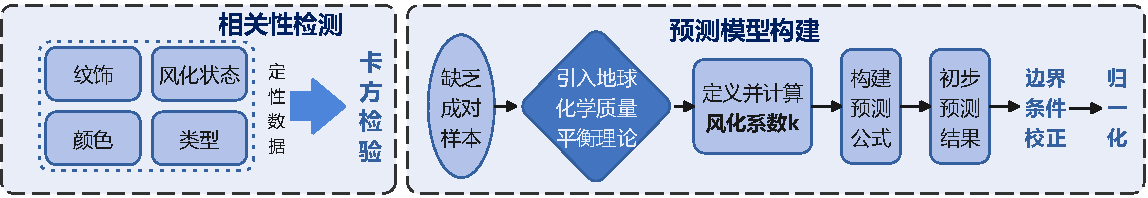
\includegraphics[width=\textwidth]{figs/3问题一/第一问框架.pdf}
	\caption{风化影响分析与成分恢复模型框架}
	\label{fig:问题一模型框架}
\end{figure}

\subsection{表面风化与文物物理属性的关联性检验}

为了探究文物表面风化现象是否与其物理属性存在关联,我们首先需要分析表面风化状态与玻璃类型、纹饰及颜色这几个变量之间的关系。这些变量的共同特征是它们均为分类变量,其取值为离散的类别而非连续的数值。

这一数据特性决定了用于衡量连续变量间线性关系的皮尔逊相关系数或用于比较组间均值差异的方差分析等方法在此并不适用,因为对“浅蓝”、“纹饰A”等类别进行数值运算不具备实际意义,需要采用一种能够处理定性数据频数的非参数检验方法来分析它们之间的关联性。因此,针对此问题,我们使用了卡方检验。

卡方检验是一种专门用于判断两个或多个分类变量之间是否存在关联的经典统计方法,其核心思想在于比较观测频数与期望频数之间的差异。其中,观测频数是样本数据中各类组合的实际计数值,而期望频数则是在“变量间相互独立”这一零假设下,根据边际概率计算出的理论计数值。检验过程通过计算两者差异的卡方统计量,并将其转换为$P$值来进行判断。在本研究中,我们设定显著性水平为$0.05$,若计算所得的$P$值小于该阈值,则拒绝变量间相互独立的零假设,认为它们之间存在显著的统计学关联。

为分析文物表面风化现象与其物理属性的关联,我们制作了关系分析的可视化图,如图\ref{fig:关系分析可视化}所示。图中第一部分展示了风化状态在两类玻璃中的分布情况。数据显示,铅钡玻璃的风化样本占其总数的73.5\%,这一比例远高于高钾玻璃的33.3\%。图中第二部分与第三部分则进一步展示了风化样本在不同纹饰和颜色类别下的数量分布。所有纹饰为B的样本均为风化样本,而纹饰为A的样本中风化与未风化数量相同。在不同颜色中,浅蓝色样本的风化数量为20,远超其未风化数量6,而蓝绿色样本中两者的数量则基本持平。这些在不同类别下风化比例与数量的显著差异直观地表明表面风化与文物的物理属性并非相互独立。





\begin{figure}[H]

\centering

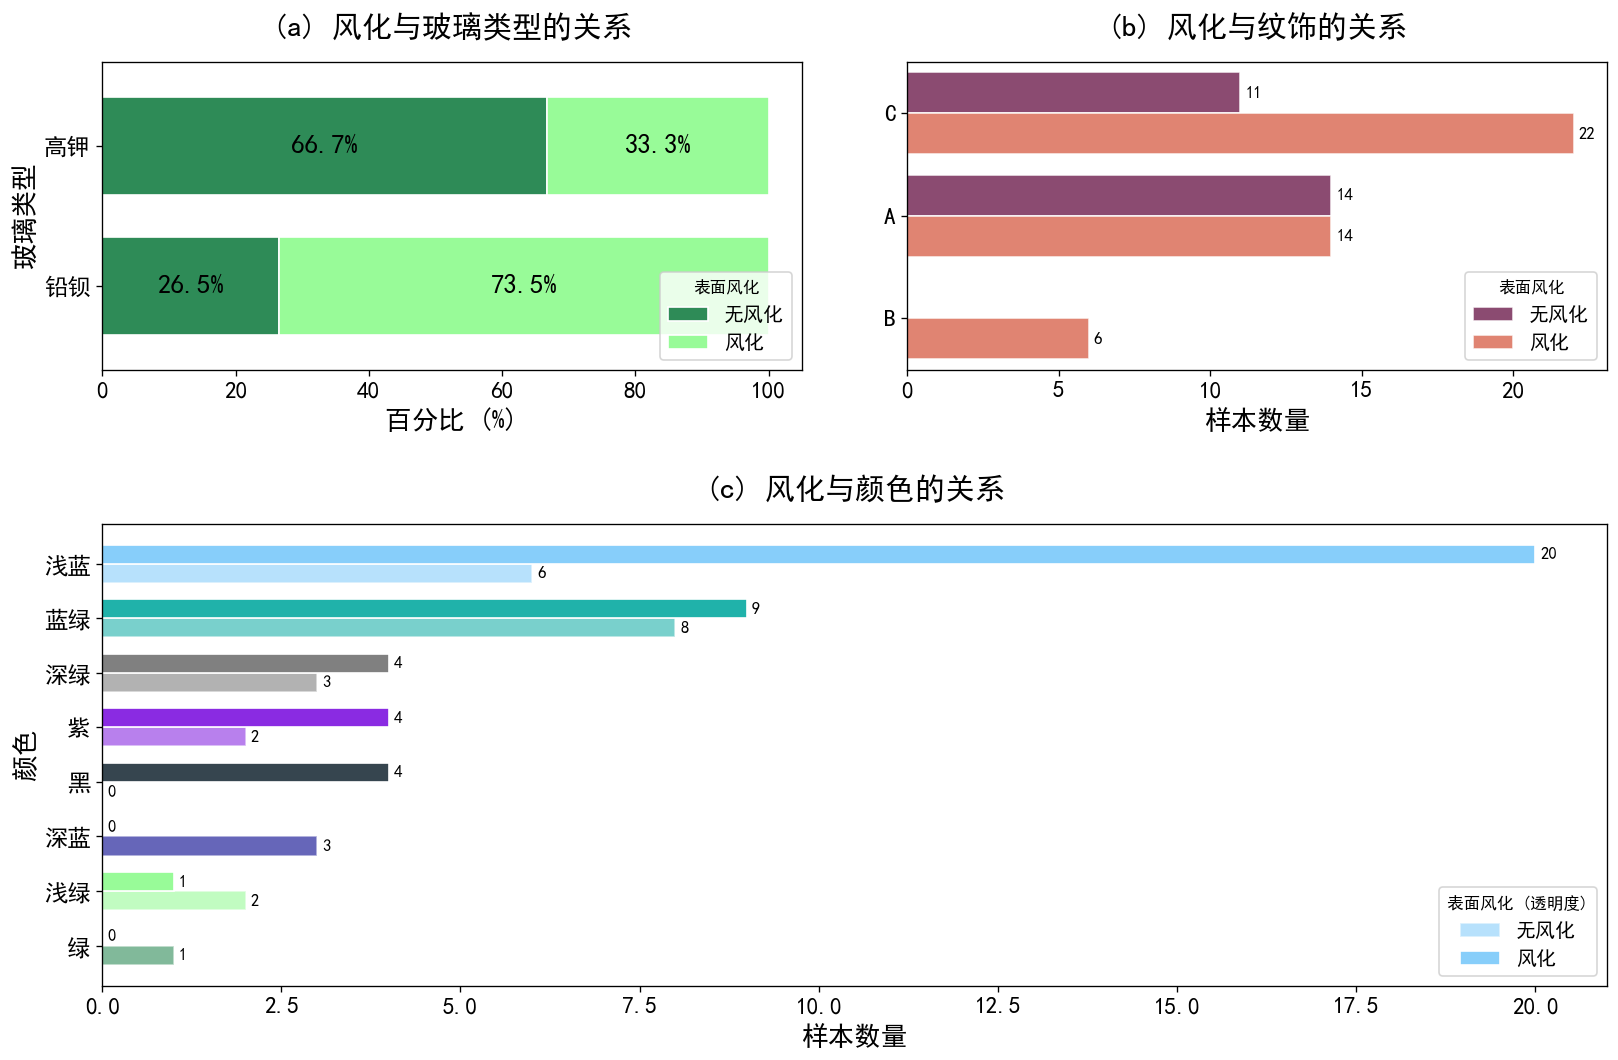
\includegraphics[width=\textwidth]{figs/3问题一/问题一_关系分析可视化_组合图_黄金分割.png}

\caption{表面风化与类型、纹饰及颜色的关系可视化}

\label{fig:关系分析可视化}

\end{figure}




\subsection{风化对两类玻璃化学成分含量的影响规律}

基于风化与玻璃类型存在关联的结论,我们进一步对风化在高钾和铅钡两类玻璃中引起的化学成分变化规律进行分析。我们将样本数据分为高钾未风化、高钾风化、铅钡未风化、铅钡风化四个组别,并对各组样本的化学成分含量分布进行了比较。

我们采用分面箱线图对两类玻璃在风化前后的化学成分分布进行可视化,如图\ref{fig:高钾玻璃成分分布}与图\ref{fig:铅钡玻璃成分分布}所示。箱线图展示了数据的中位数、四分位距和离散程度。从图中可以观察到,对于高钾玻璃,风化作用导致氧化钾$K_2O$的含量中位数显著下降,而氧化硅$SiO_2$的含量则有上升趋势。对于铅钡玻璃,风化作用主要表现为氧化铅$PbO$与氧化钡$BaO$含量的大幅降低,同时氧化硅$SiO_2$含量相应增加。这种变化说明风化过程中发生了元素的选择性流失与富集。

\begin{figure}[H]
	\centering
	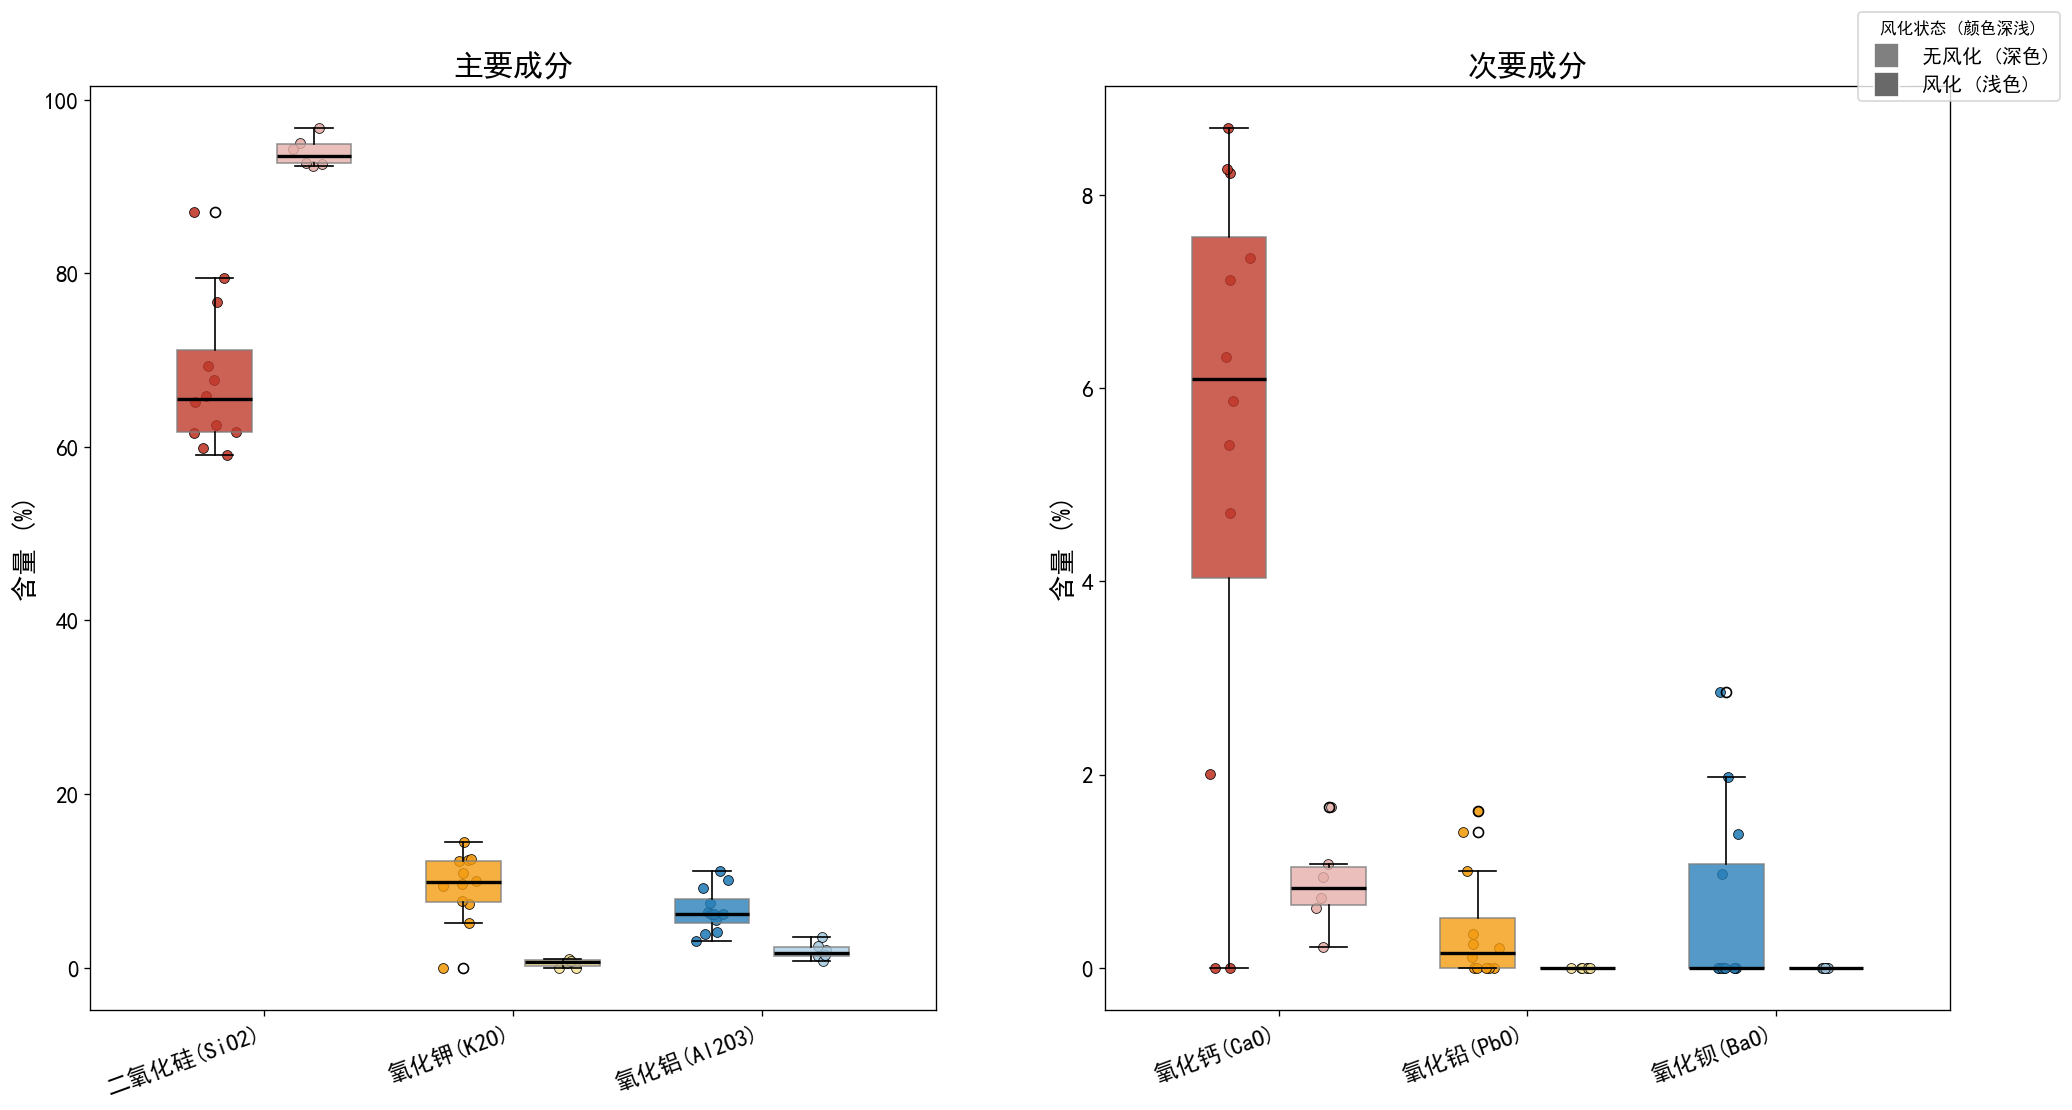
\includegraphics[width=\textwidth]{figs/3问题一/高钾玻璃成分分布.png}
	\caption{高钾玻璃在风化前后各化学成分含量分布}
	\label{fig:高钾玻璃成分分布}
\end{figure}

\begin{figure}[H]
	\centering
	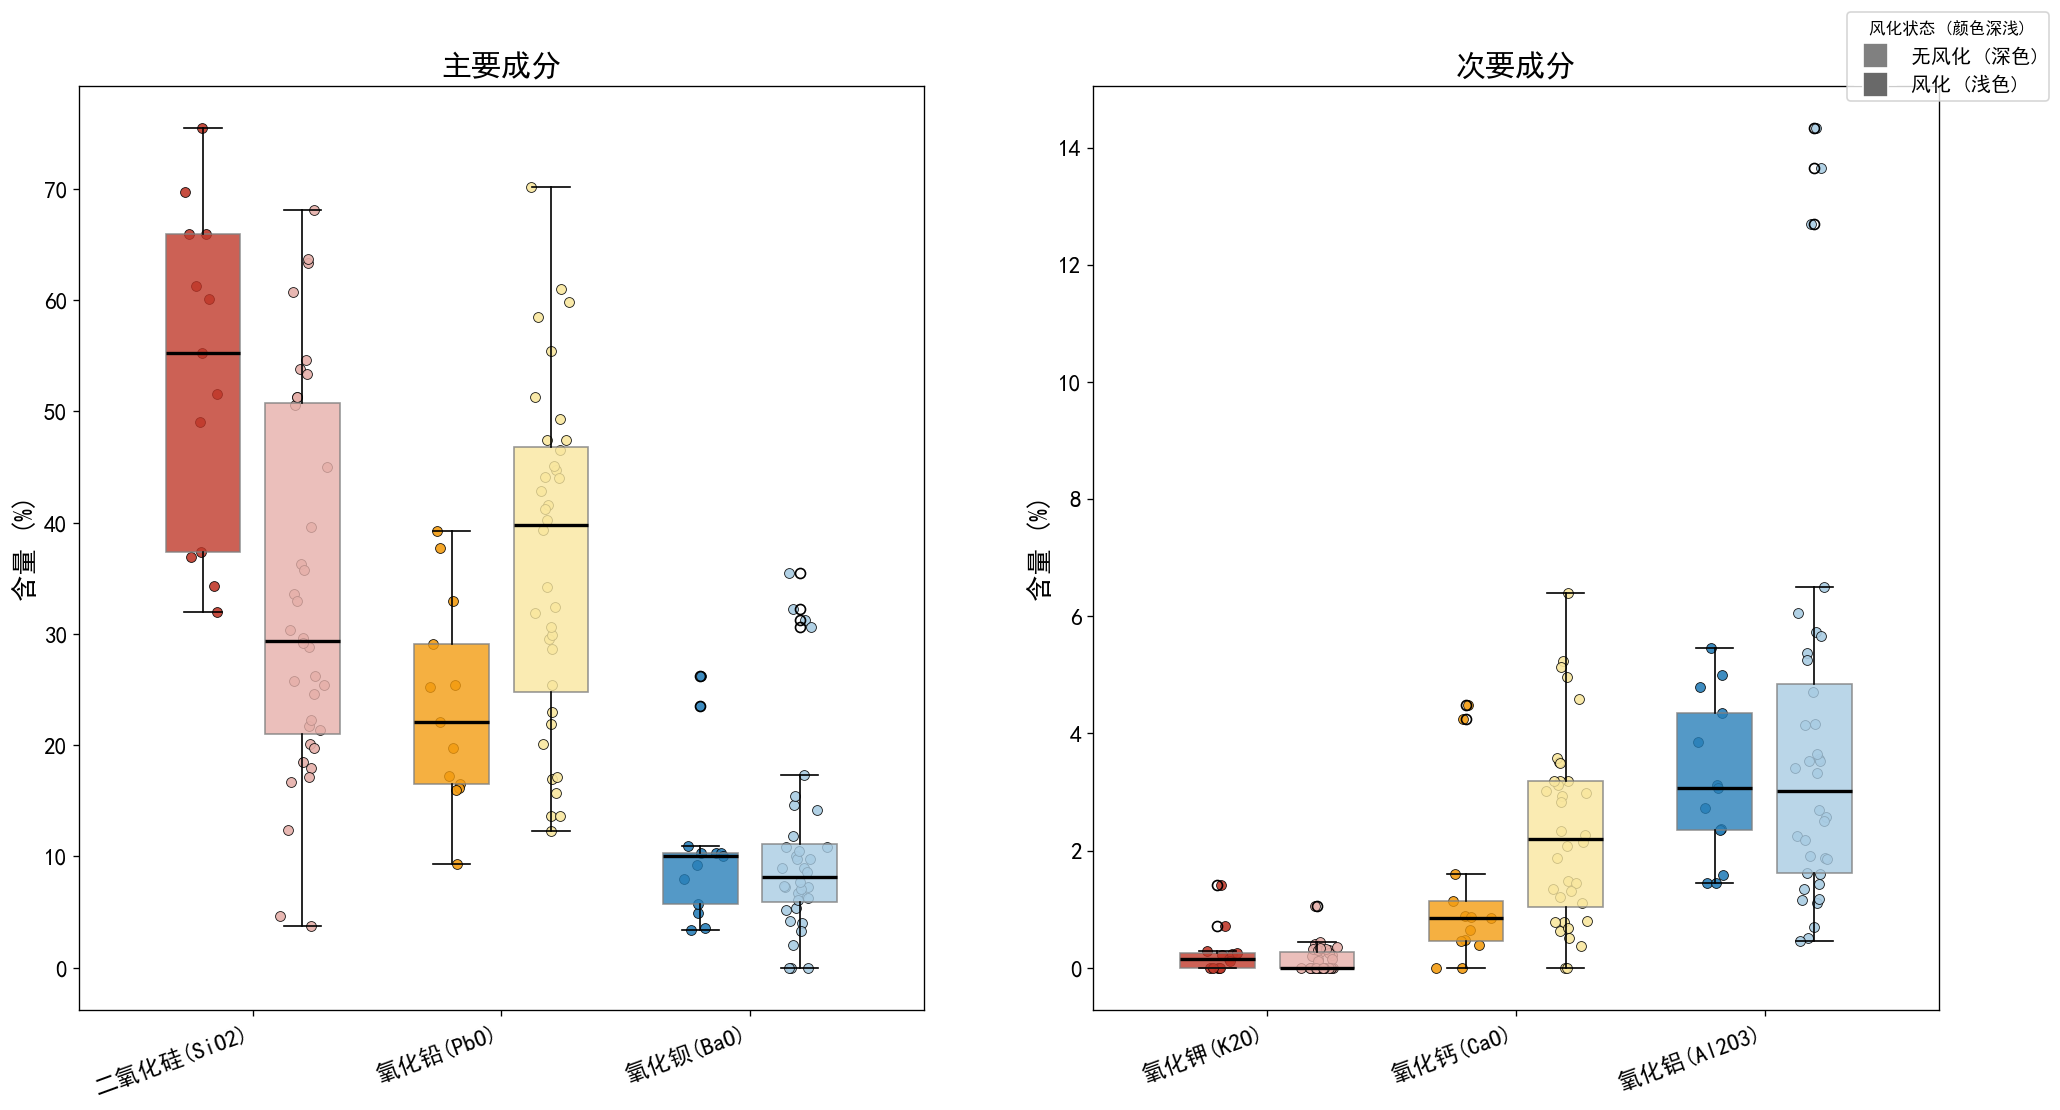
\includegraphics[width=\textwidth]{figs/3问题一/铅钡玻璃成分分布.png}
	\caption{铅钡玻璃在风化前后各化学成分含量分布}
	\label{fig:铅钡玻璃成分分布}
\end{figure}


为了更细致地观察关键化学成分的分布形态变化,我们绘制了部分核心化学成分,包括氧化铅$PbO$、氧化钾$K_2O$、氧化钡$BaO$以及二氧化硅$SiO_2$的分布图,如图\ref{fig:pbo_dist}至图\ref{fig:sio2_dist}所示。图中包含直方图与核密度估计曲线,它们共同描述了数据分布的集中趋势和形态。分析这些分布图可以发现,高钾玻璃在风化后,其氧化钾$K_2O$的含量分布从一个较宽的区间转化至接近零值的极低水平。对于铅钡玻璃,风化作用使其特征成分氧化铅$PbO$与氧化钡$BaO$的含量分布整体向低值区移动。与此相反,作为玻璃基体的二氧化硅$SiO_2$,其含量分布在两类玻璃中均表现出向高值区偏移的趋势,说明在风化过程中其他元素的流失导致了二氧化硅的相对富集。


\begin{figure}[H]
	\centering
	\begin{minipage}{0.48\textwidth}
		\centering
		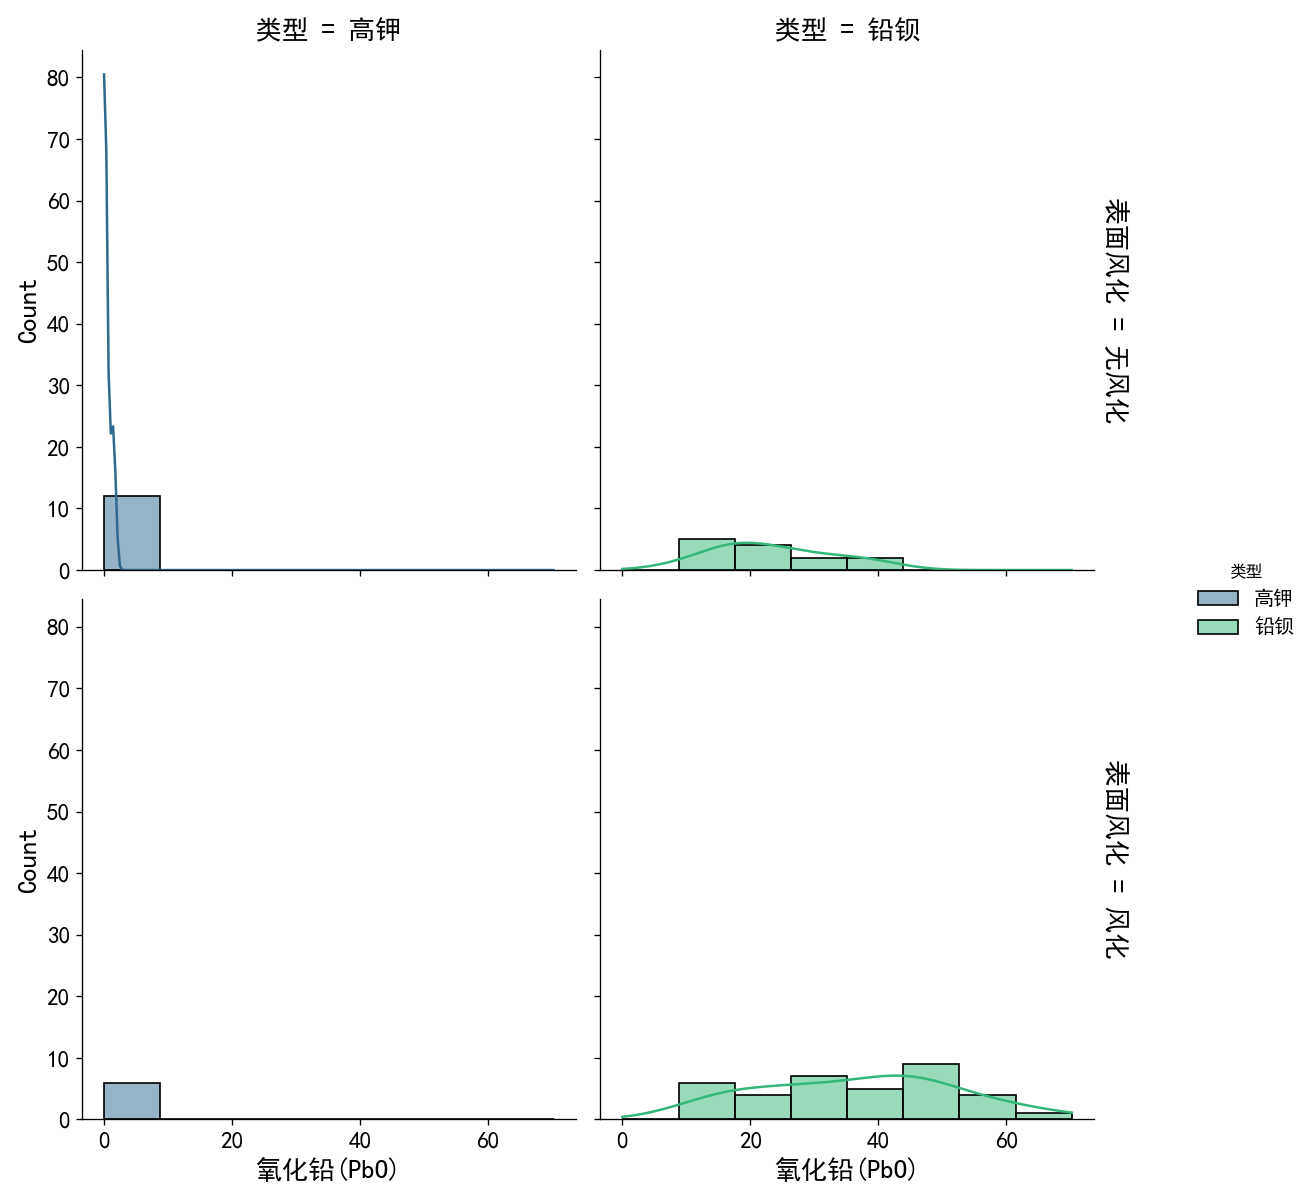
\includegraphics[width=\linewidth]{figs/3问题一/分布图_氧化铅(PbO).png}
		\caption{氧化铅$PbO$含量分布}
		\label{fig:pbo_dist}
	\end{minipage}\hfill
	\begin{minipage}{0.48\textwidth}
		\centering
		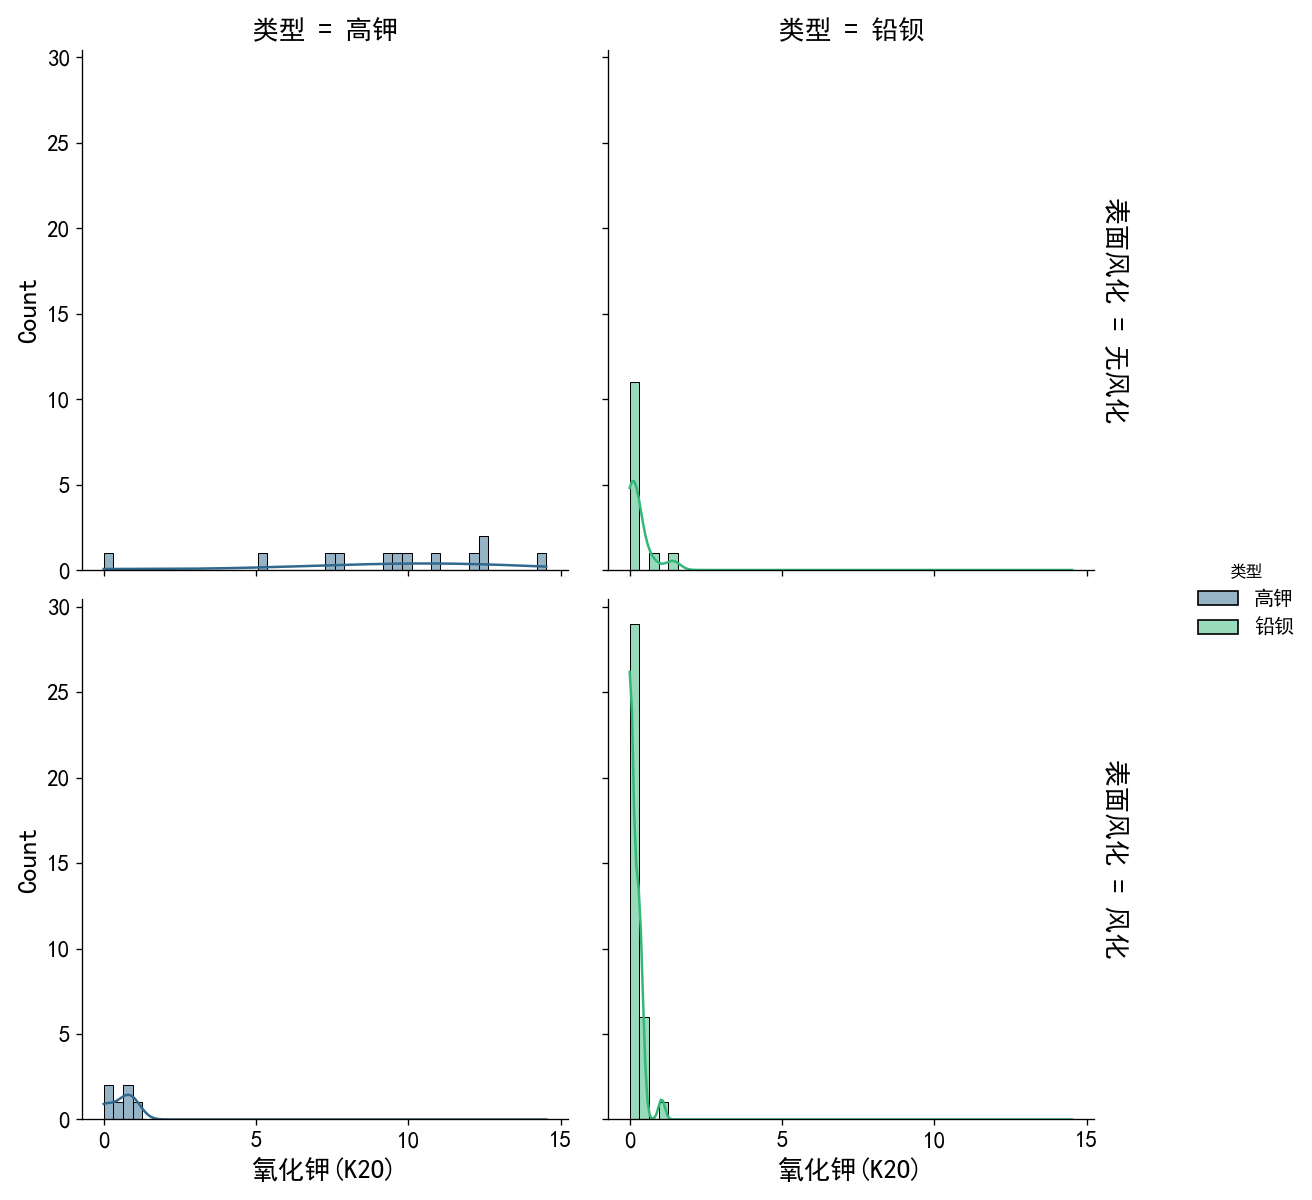
\includegraphics[width=\linewidth]{figs/3问题一/分布图_氧化钾(K2O).png}
		\caption{氧化钾$K_2O$含量分布}
		\label{fig:k2o_dist}
	\end{minipage}
\end{figure}

\begin{figure}[H]
	\centering
	\begin{minipage}{0.48\textwidth}
		\centering
		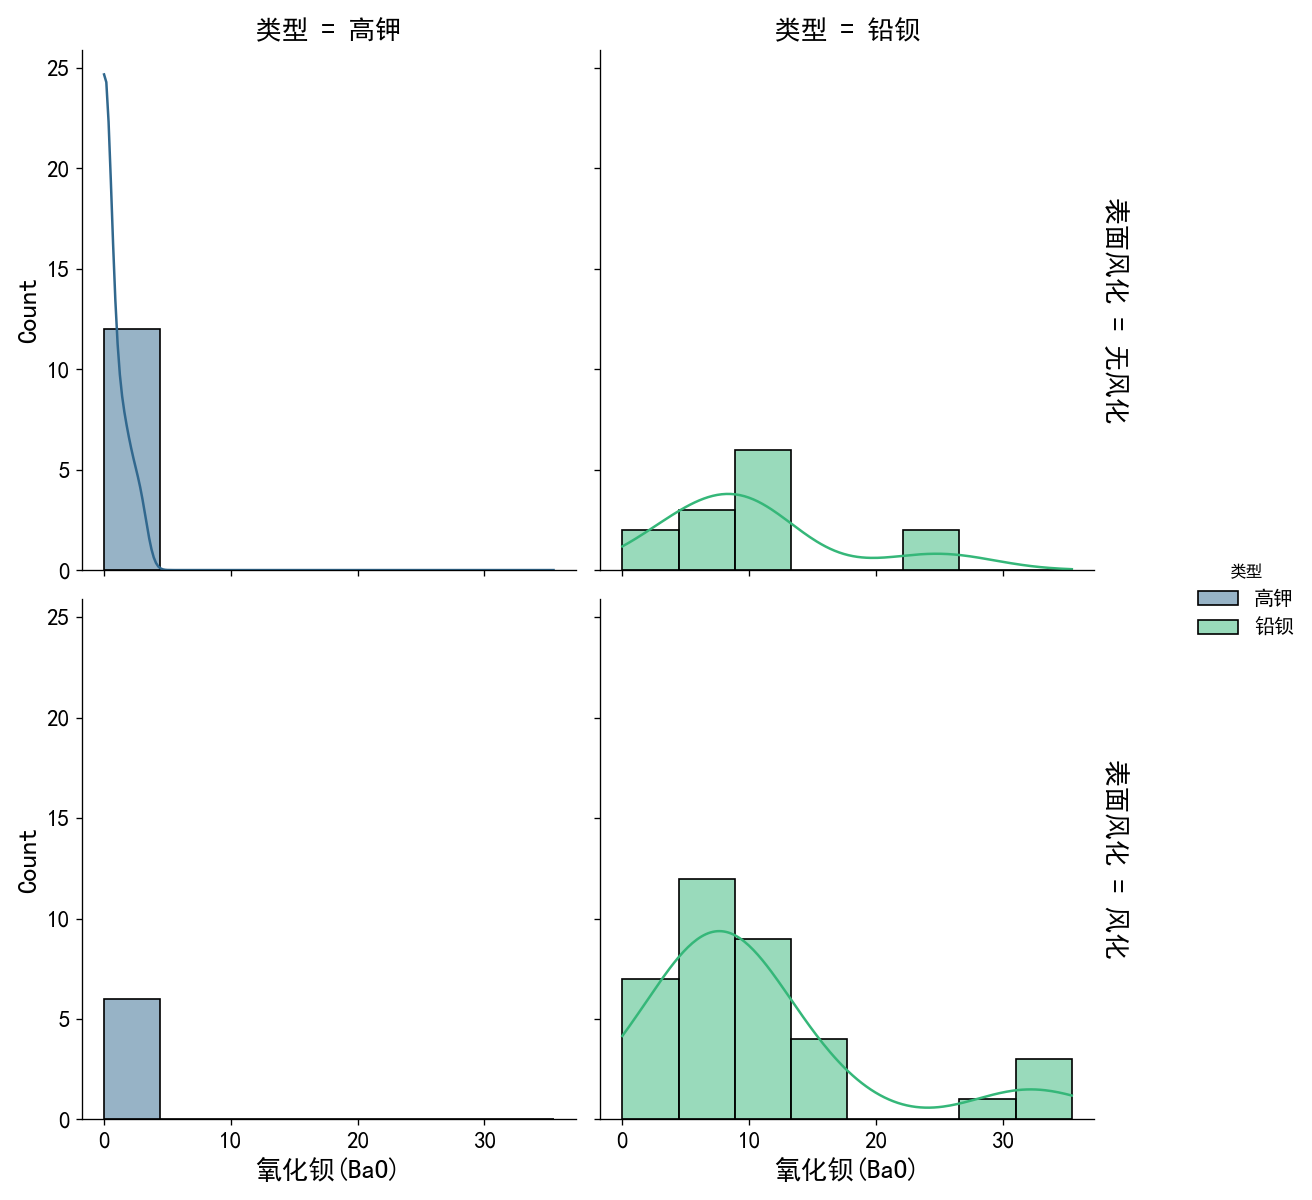
\includegraphics[width=\linewidth]{figs/3问题一/分布图_氧化钡(BaO).png}
		\caption{氧化钡$BaO$含量分布}
		\label{fig:bao_dist}
	\end{minipage}\hfill
	\begin{minipage}{0.48\textwidth}
		\centering
		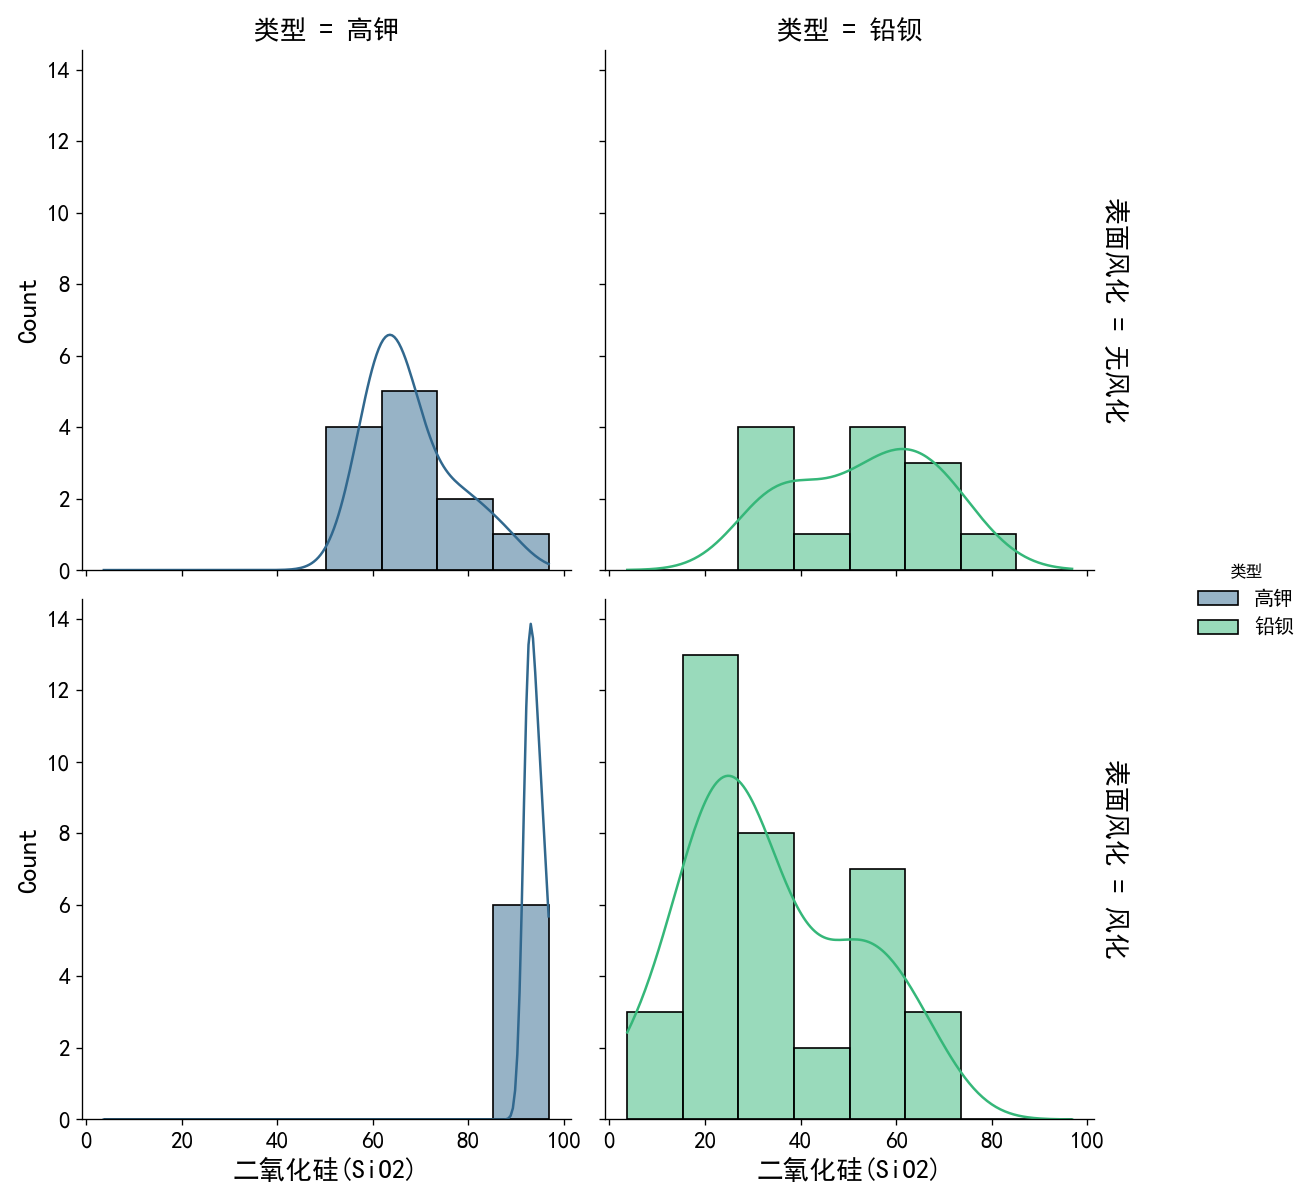
\includegraphics[width=\linewidth]{figs/3问题一/分布图_二氧化硅(SiO2).png}
		\caption{二氧化硅$SiO_2$含量分布}
		\label{fig:sio2_dist}
	\end{minipage}
\end{figure}

\subsection{基于风化系数的化学成分含量预测模型}

预测风化前化学成分的主要困难在于数据中缺乏源自同一文物的风化与未风化的观测样本。这使得依赖大量成对样本进行训练的传统监督学习模型,例如回归分析,难以直接应用且存在较高的过拟合风险。

于是,我们转向从风化过程的物理化学机理中寻求建模依据。玻璃的风化过程与地质学中岩石的蚀变过程在原理上具有相似性,均为长期化学环境作用下的元素迁移过程。因此,我们引入了地球化学领域成熟的质量平衡分析理论来构建预测模型,该理论能够在缺乏直接演变过程数据时,对成分变化进行有效推断。

我们的模型的核心假设为:特定化学成分在风化过程中的流失或富集比例,与其在未风化状态下的原始含量相关。此假设参考了地质学中分析交代蚀变作用的艾索康图法的原理,它将风化视为一个系统性的化学变化过程而非随机过程,从而建立了基于风化系数的预测方法。

我们首先为每种玻璃类型$t$和每种化学成分$j$定义一个风化系数$k_{t,j}$。该系数由该类型玻璃中所有风化样本与未风化样本的平均含量计算得出,其数学表达式如下:
\begin{equation}
	k_{t,j} = 1 - \frac{\bar{C}_{t,j,\text{weathered}}}{\bar{C}_{t,j,\text{unweathered}}}
\end{equation}
其中,$\bar{C}_{t,j,\text{weathered}}$表示$t$类玻璃风化样本中$j$成分的平均含量,$\bar{C}_{t,j,\text{unweathered}}$表示$t$类玻璃未风化样本中$j$成分的平均含量。

利用计算得到的风化系数,我们可以对任意一个已知风化后成分含量$C_{\text{weathered}, j}$的样本,进行其风化前含量$C'_{\text{unweathered}, j}$的初步预测,其预测公式为:
\begin{equation}
	C'_{\text{unweathered}, j} = \frac{C_{\text{weathered}, j}}{1 - k_{t,j}}
\end{equation}

考虑到测量误差和模型的局限性,初步预测得到的各成分总和可能偏离100\%。因此,我们对预测结果进行了边界条件校正。我们计算所有预测成分的总和,并进行条件归一化处理,以确保最终得到的预测成分总和落入题目要求的85\%至105\%的有效区间内,从而使预测结果在化学上更具合理性。模型的最终预测结果,以原始含量和预测含量并列对比的形式,被完整地保存至\texttt{Result/问题一\_预测结果.xlsx}文件中。


\section{问题二:玻璃文物分类、亚类划分及可靠性分析}

本部分的目标是根据文物的化学成分,建立高钾玻璃与铅钡玻璃的分类规律,并对两类玻璃进行内部亚类的划分,最后对所得结论的可靠性进行系统性分析。其框架如图\ref{fig:problem2_framework}所示。

\begin{figure}[H]
    \centering
    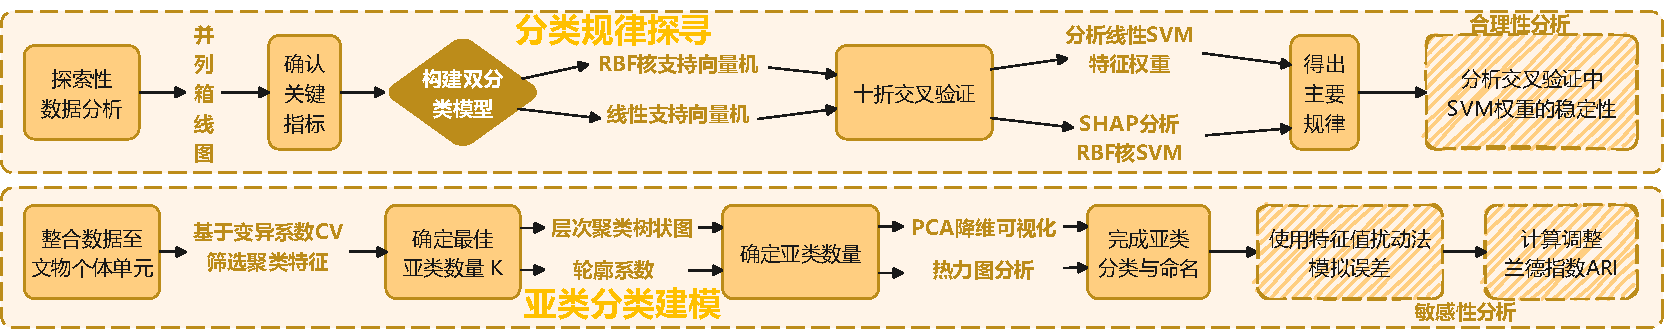
\includegraphics[width=\textwidth]{figs/4问题二/第二问框架.pdf}
    \caption{问题二框架}
    \label{fig:problem2_framework}
\end{figure}

\subsection{高钾玻璃与铅钡玻璃的分类规律}

在构建分类模型之前,首先需要通过探索性数据分析对不同类别的数据在数值特征上的分布差异建立直观认知,这为后续的建模方向和假设形成提供依据。我们采用并列箱线图来直观对比高钾玻璃与铅钡玻璃在全部十四种化学成分含量上的分布差异。

\begin{figure}[H]
    \centering
    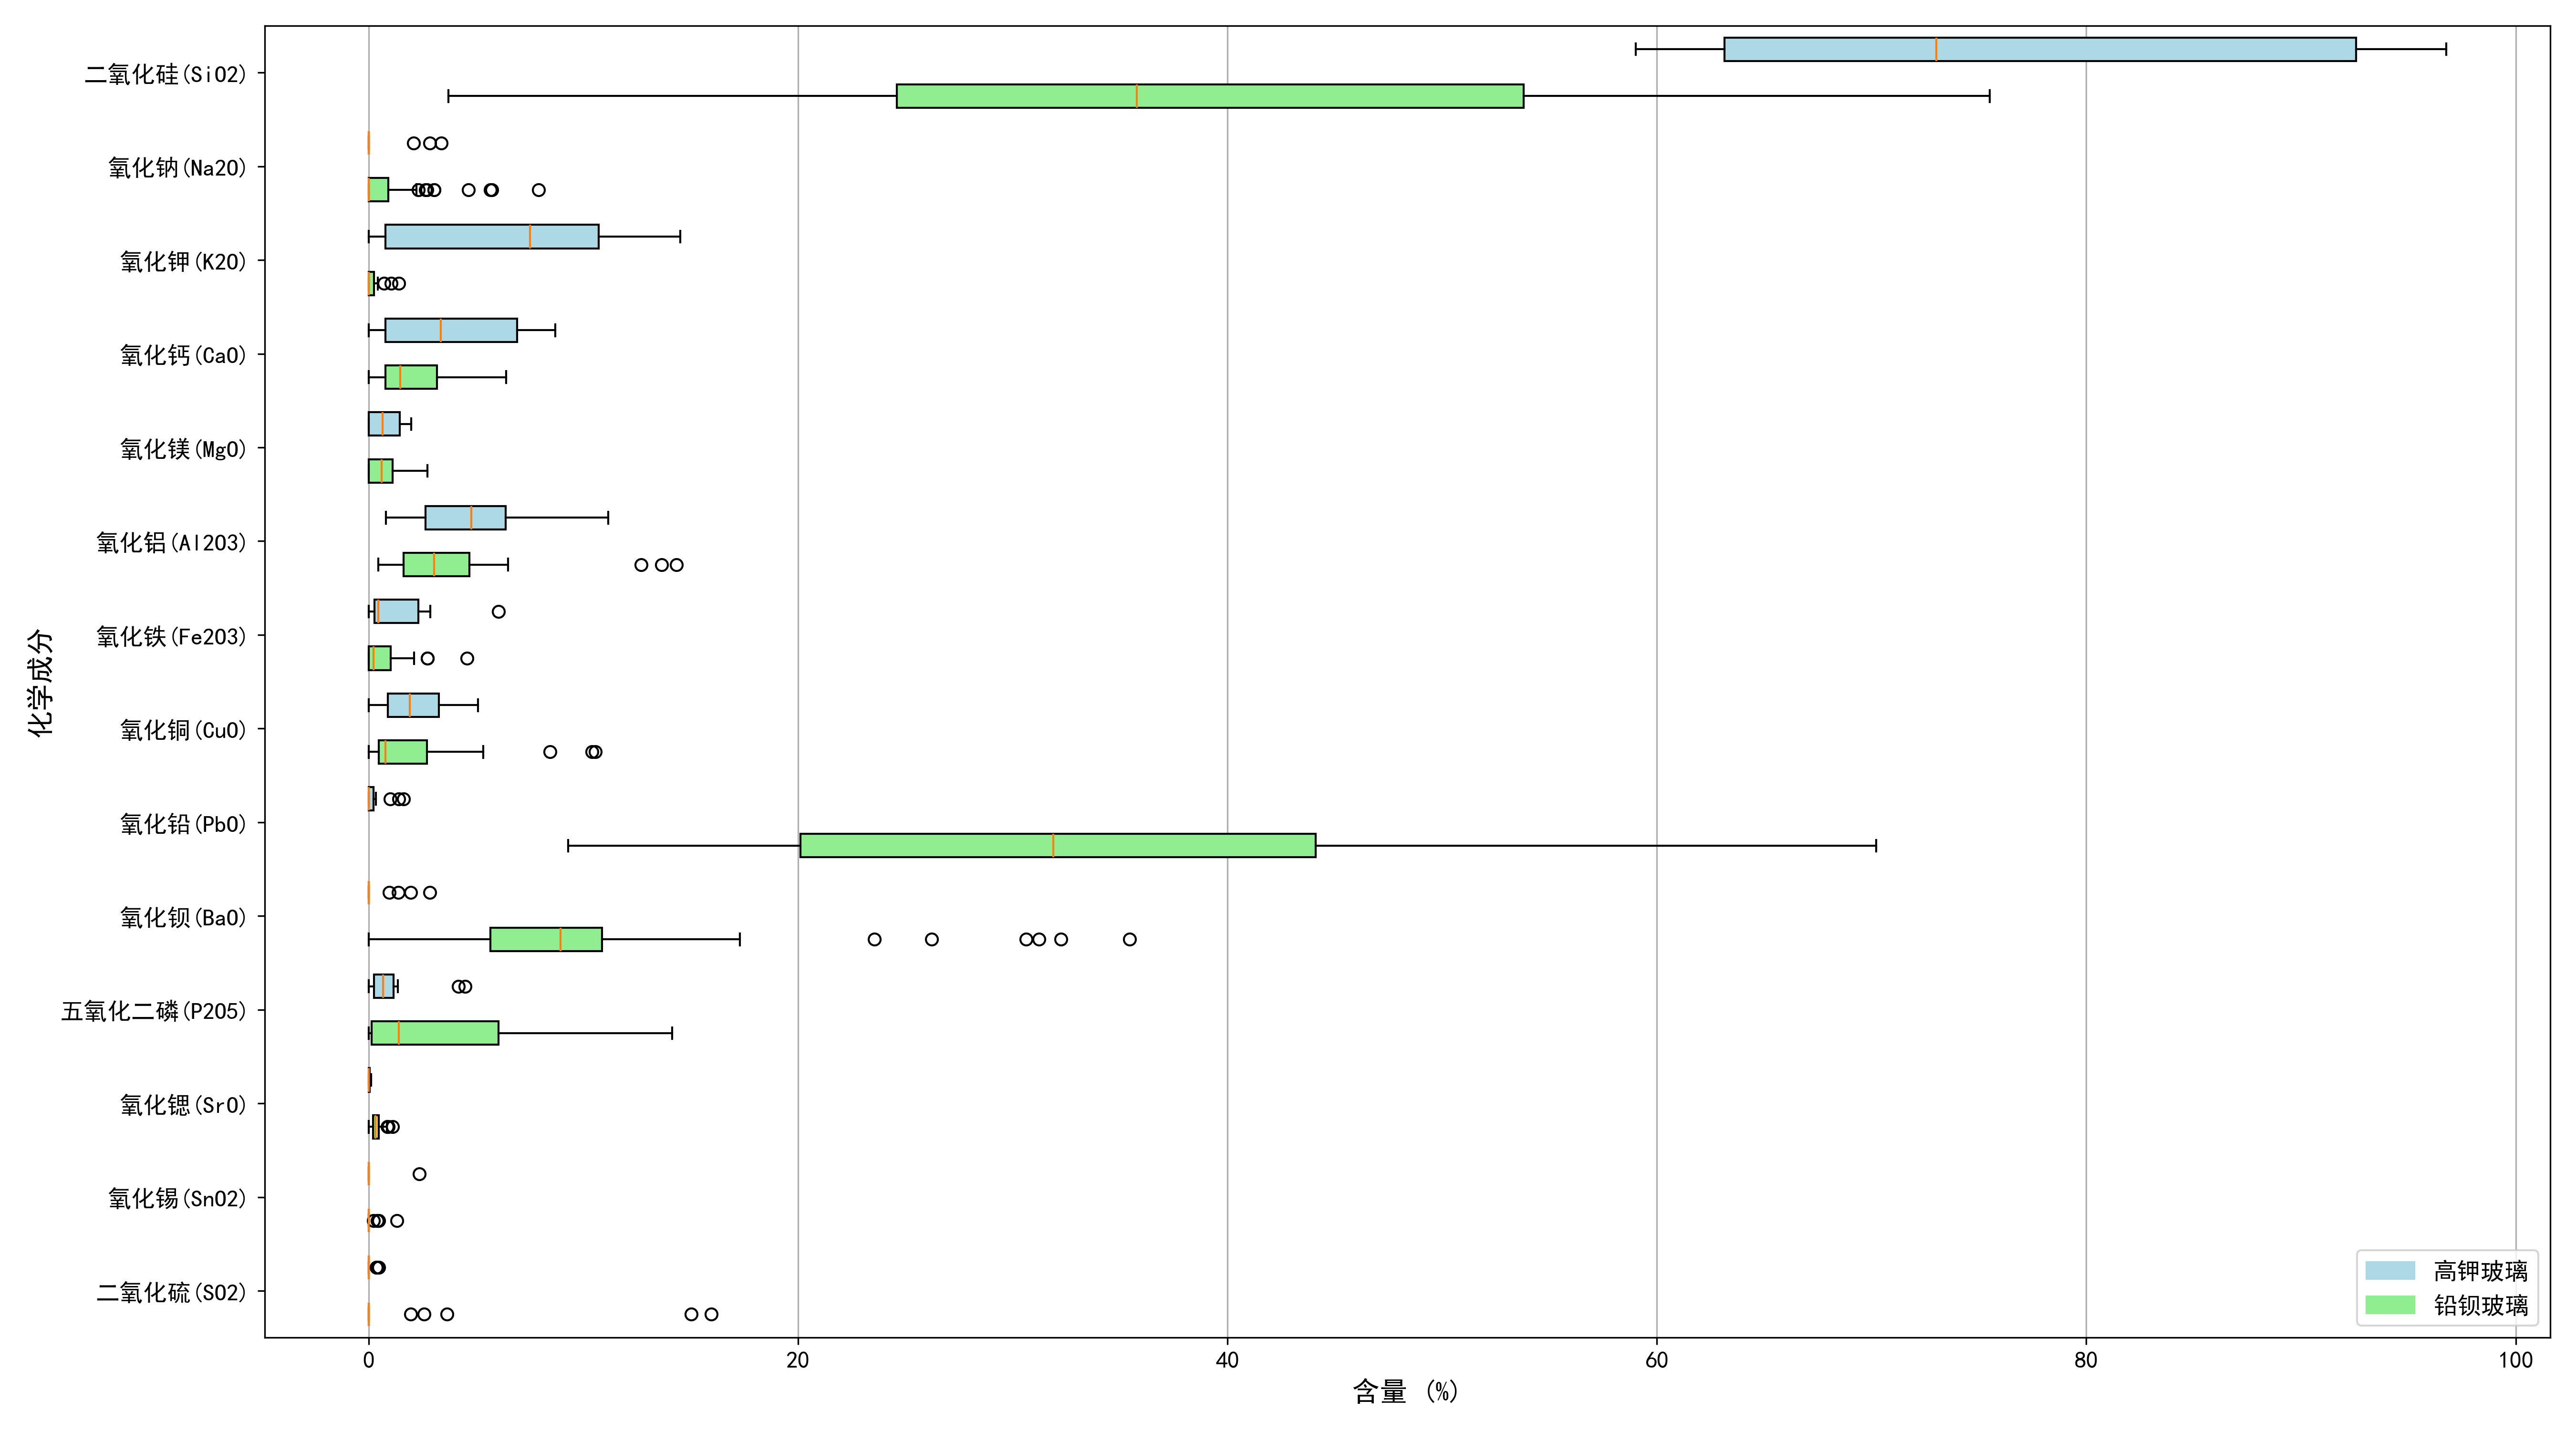
\includegraphics[width=\textwidth]{figs/4问题二/EDA_并列箱线图.png}
    \caption{高钾玻璃与铅钡玻璃化学成分含量分布对比}
    \label{fig:eda_boxplot}
\end{figure}

如图\ref{fig:eda_boxplot}所示,图中纵轴为化学成分,横轴为含量百分比。对于每一种成分,均并排展示了两个箱体,分别代表高钾玻璃和铅钡玻璃的含量分布。由图可知,在氧化铅$PbO$与氧化钡$BaO$两种成分上,铅钡玻璃的含量分布远高于高钾玻璃,而在氧化钾$K_2O$上则呈现相反的模式。两个类别在这些关键成分上的分布区间几乎没有重叠,由此形成核心假设,即$PbO$、$BaO$与$K_2O$是区分两类玻璃的关键指标。

基于前述探索性分析形成的假设,即特定化学成分含量可有效区分玻璃类型,我们构建监督学习分类模型以对该规律进行量化验证。为兼顾模型的解释性与对数据复杂关系的拟合能力,我们分别建立了线性支持向量机与使用径向基函数核的非线性支持向量机模型。

线性支持向量机的基本原理是在一个多维特征空间中,寻找一个最优的分类超平面。该超平面由法向量$\boldsymbol{w}$和位移$b$定义,其数学形式为$\boldsymbol{w}^T\boldsymbol{x} + b = 0$。最优化的目标是不仅能将两类样本分开,同时能最大化距离超平面最近的样本,即支持向量,到超平面的间隔。在允许部分样本被错误分类以增强模型泛化能力的情况下,该问题可表述为一个软间隔优化问题,其目标函数如下
\begin{equation}
    \min_{\boldsymbol{w}, b, \boldsymbol{\xi}} \frac{1}{2} ||\boldsymbol{w}||^2 + C \sum_{i=1}^{m} \xi_i
\end{equation}
式中$C$为正则化系数,用于平衡间隔最大化与分类误差,$\xi_i$是松弛变量,允许样本点在一定程度上偏离其正确的分类边界。

当化学成分与玻璃类型的关系无法通过线性边界有效分离时,需要引入非线性模型。非线性支持向量机通过核技巧将原始特征空间映射到一个更高维度的空间,并在新空间中构造线性超平面。我们选用径向基函数核,即高斯核,作为映射函数,其定义为
\begin{equation}
    K(\boldsymbol{x}_i, \boldsymbol{x}_j) = \exp(-\gamma ||\boldsymbol{x}_i - \boldsymbol{x}_j||^2)
\end{equation}
其中$\gamma$是核函数的一个参数,它决定了单个训练样本影响范围的大小。通过使用该核函数,模型能够在原始空间中形成复杂的非线性决策边界。

为获得稳健的模型性能评估,避免因单次数据划分带来的偶然性,我们采用十折交叉验证方法。该方法将数据集随机分为十个互斥的子集,轮流使用其中九个作为训练集,一个作为测试集,最终以十次测试结果的平均值作为模型的性能度量。评估结果显示,线性支持向量机模型的平均分类准确率为95.71\%,而使用径向基函数核的非线性支持向量机模型平均分类准确率达到97.41\%。两个模型均表现出较高的分类能力。

为解释模型的分类机理,我们首先分析了线性支持向量机学习到的特征权重。

\begin{figure}[H]
    \centering
    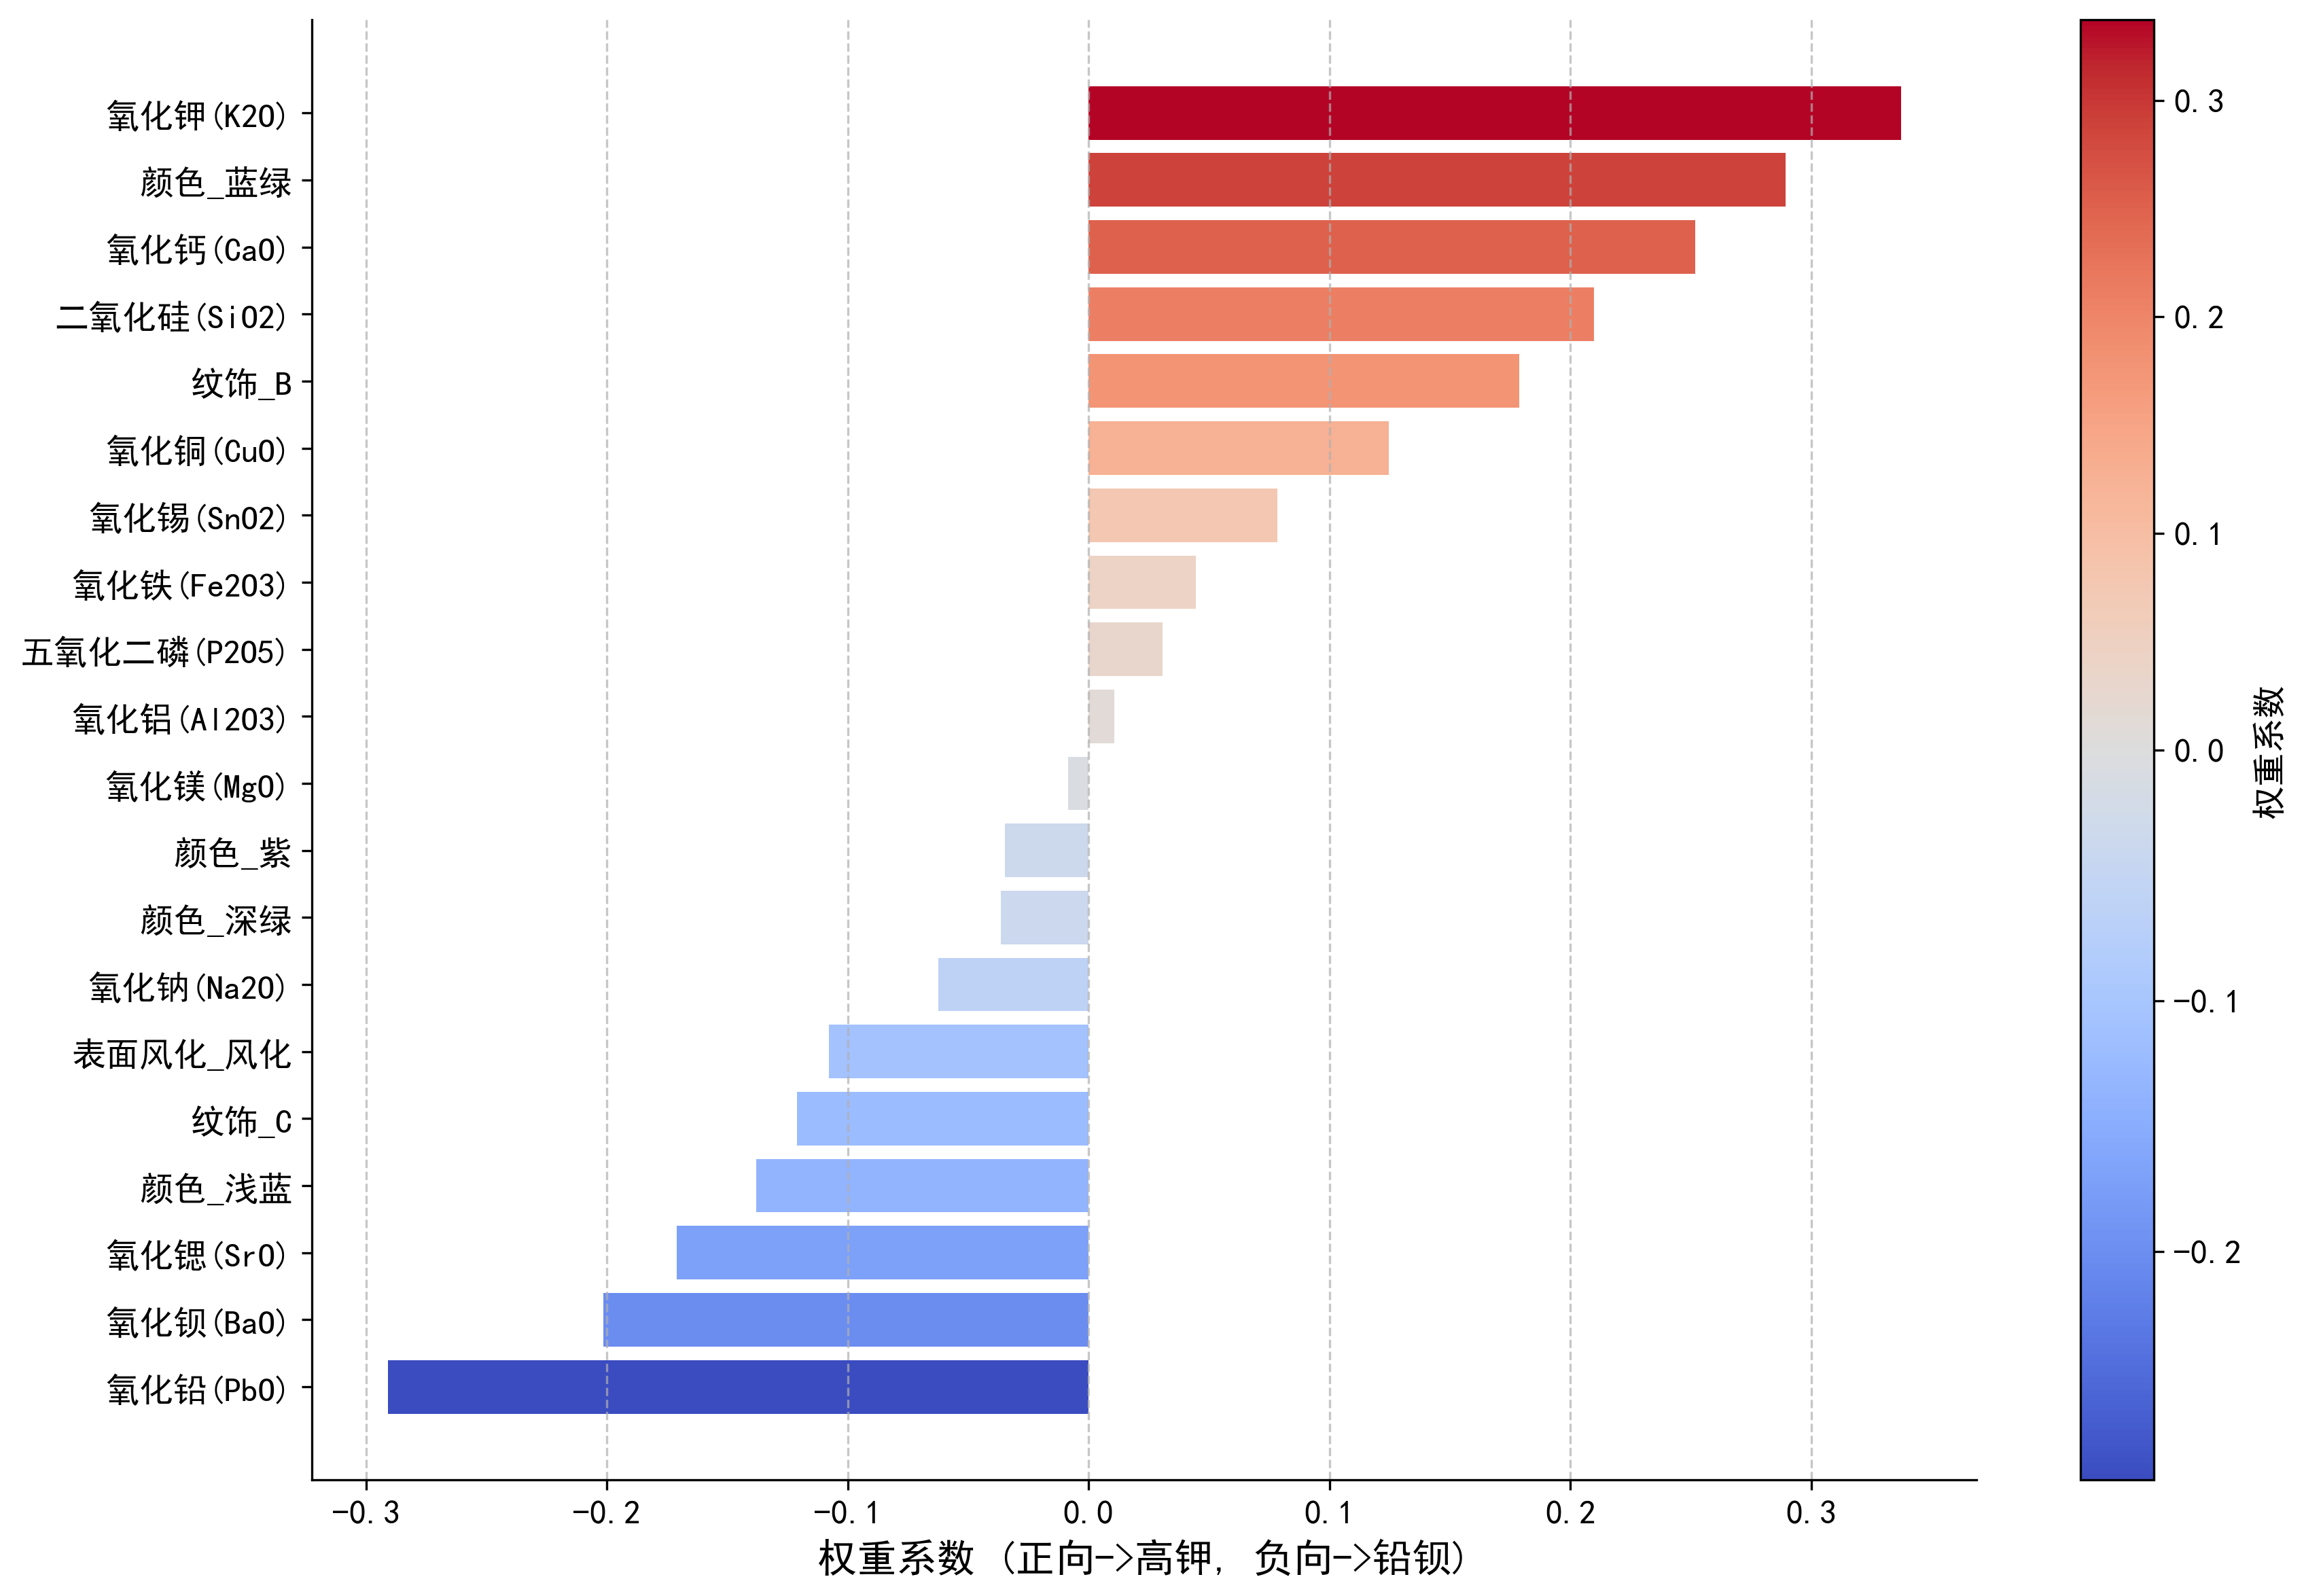
\includegraphics[width=\textwidth]{figs/4问题二/线性SVM特征权重_渐变色.png}
    \caption{线性支持向量机模型学习的特征权重}
    \label{fig:svm_weights}
\end{figure}

图\ref{fig:svm_weights}展示了各化学成分的权重系数值,其中正向权重将预测推向高钾玻璃,负向权重则推向铅钡玻璃。图中可见,氧化钾$K_2O$与二氧化硅$SiO_2$获得了最大的正权重,而氧化铅$PbO$与氧化钡$BaO$获得了最大的负权重,这与探索性分析的发现一致。

对于性能更高但解释性较弱的非线性模型,我们采用SHAP,即SHapley Additive exPlanations框架进行分析。该方法基于合作博弈论,能够将模型的预测结果公平地归因到每个输入特征上。

\begin{figure}[H]
    \centering
    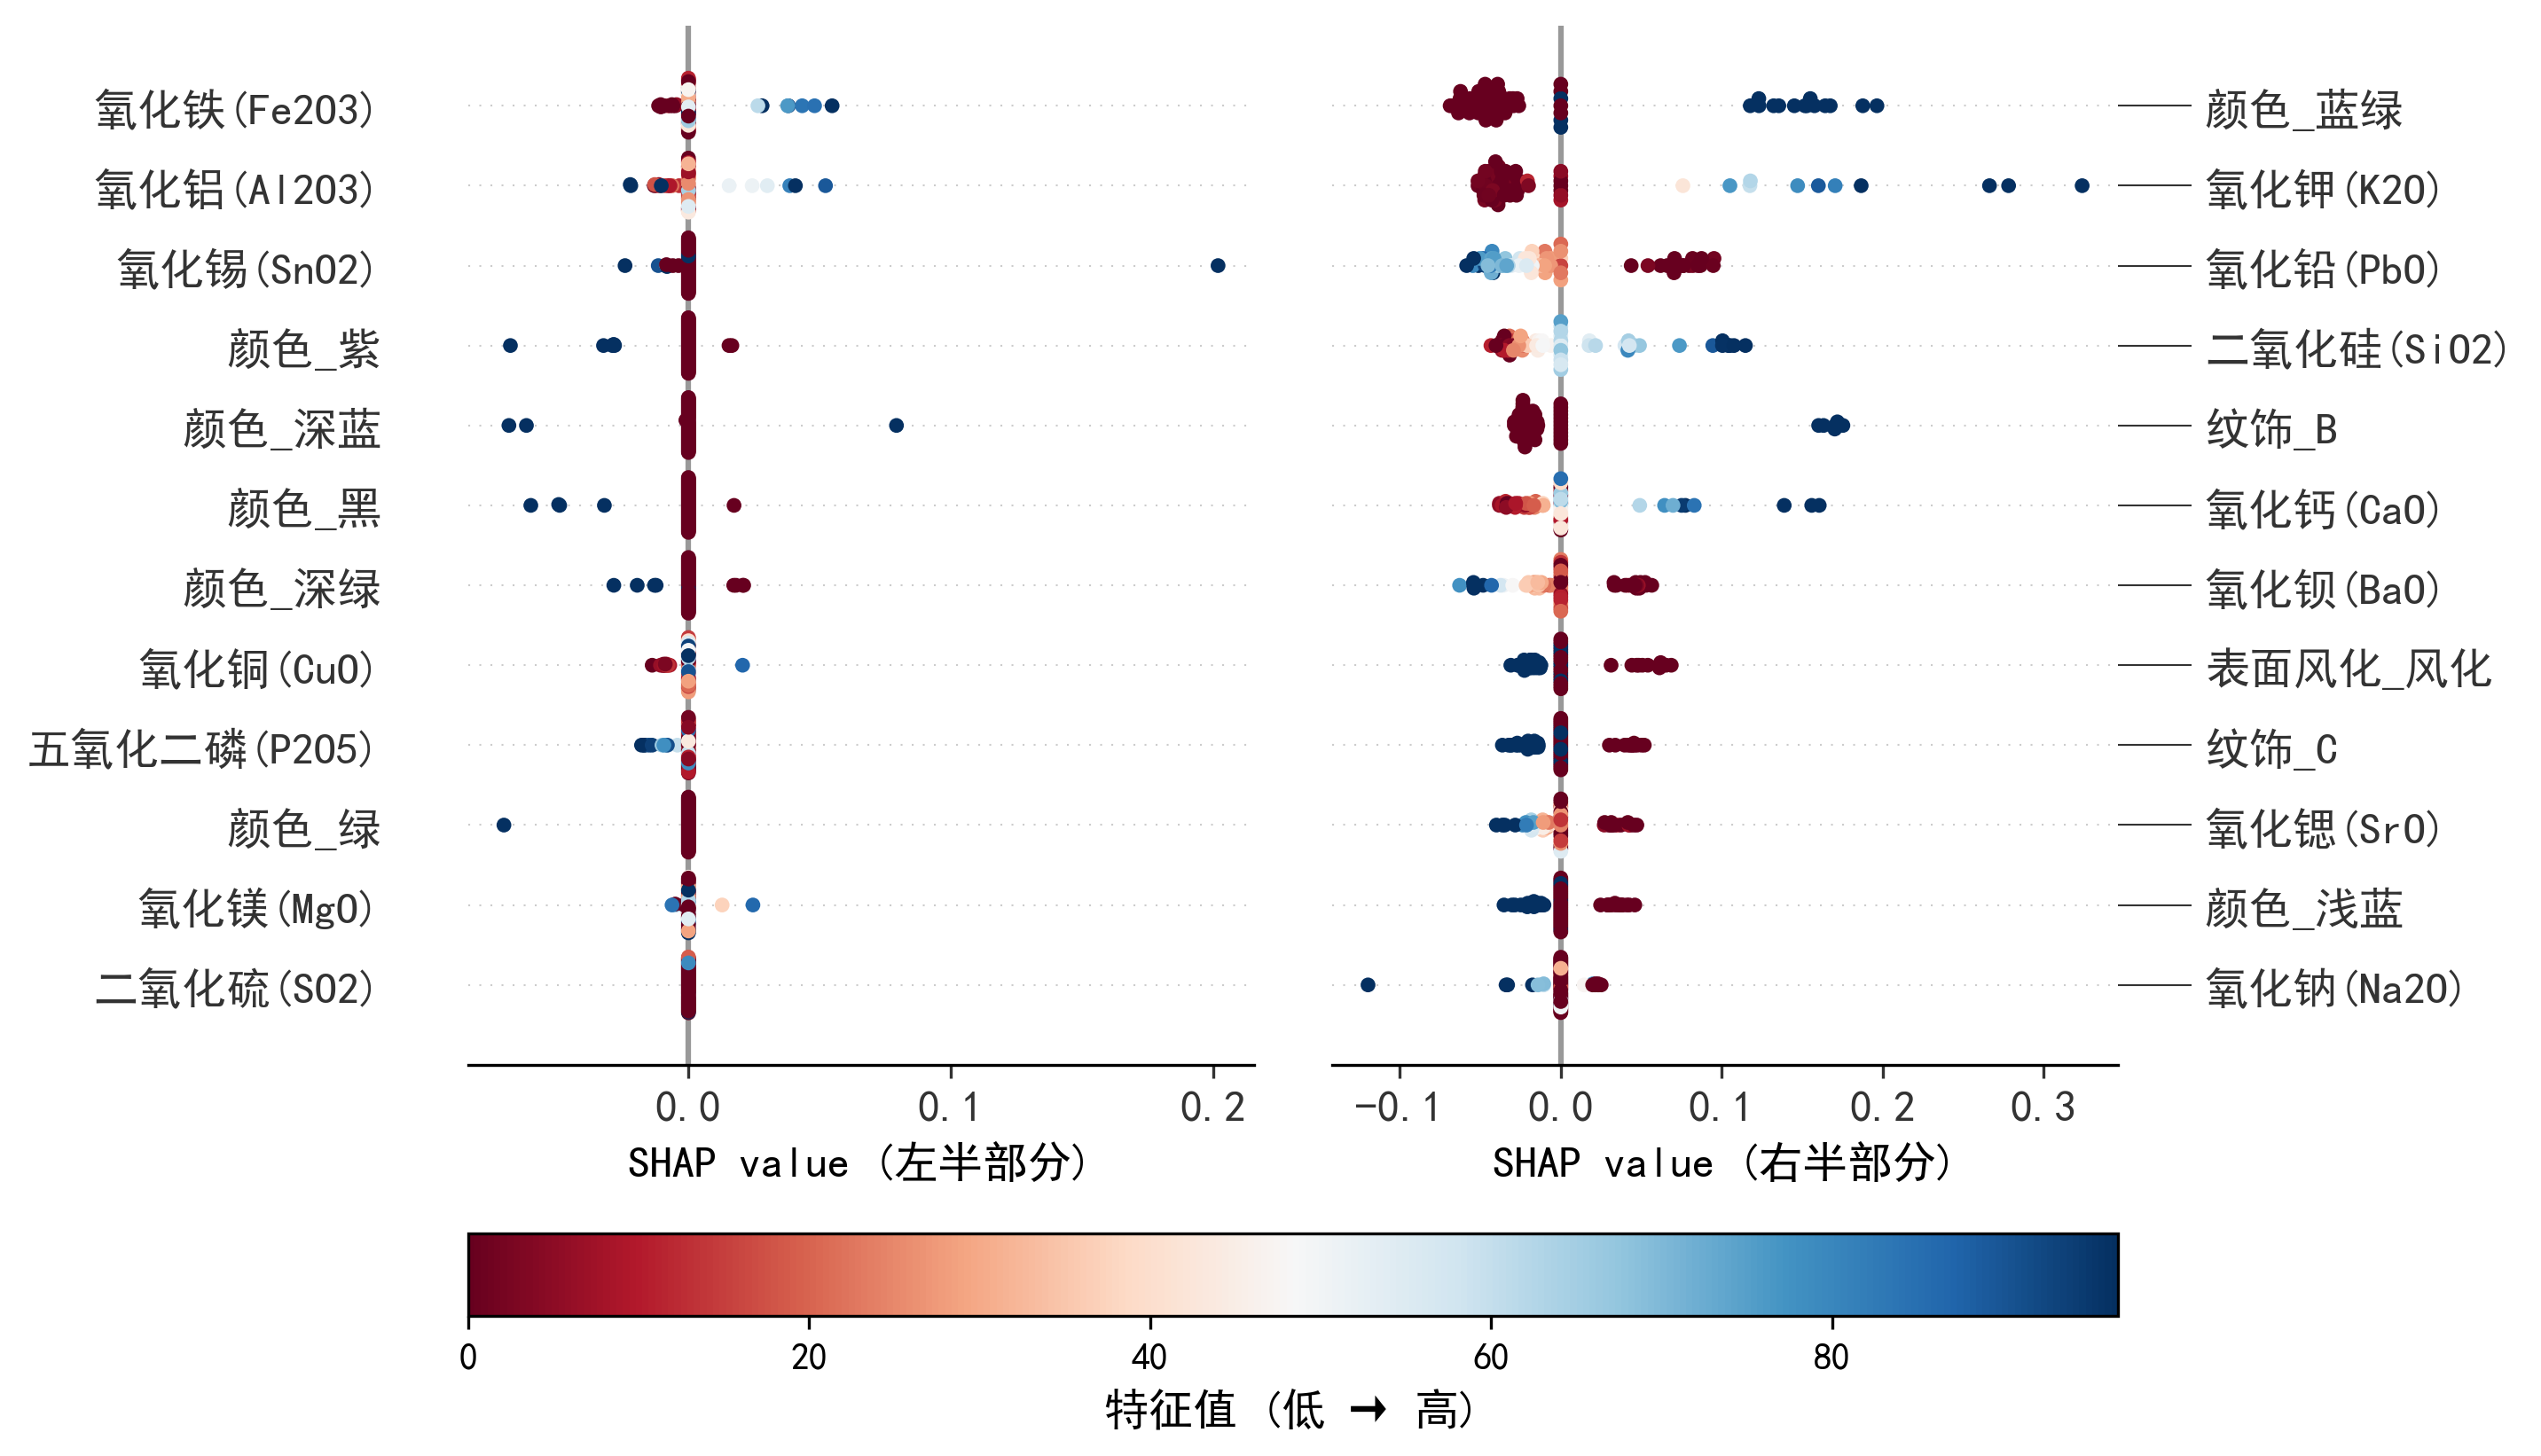
\includegraphics[width=\textwidth]{figs/4问题二/SHAP摘要图_双列_最终版_横置色条.png}
    \caption{非线性支持向量机模型的SHAP全局特征重要性分析}
    \label{fig:shap_summary}
\end{figure}

图\ref{fig:shap_summary}展示了全局特征重要性,纵轴按重要性高低排列特征,横轴是SHAP值,点的颜色代表该特征原始值的大小。该图再次确认$PbO$与$K_2O$是最重要的特征,并且提供了更丰富的细节,高含量的$PbO$红点总是对应着强烈的负向SHAP值,而高含量的$K_2O$红点则总是对应着强烈的正向SHAP值。

\subsection{各类别内部的亚类划分}

亚类划分的目标是探索同一类别文物之间是否存在基于化学成分的更细微群组。因此,分析的最小单元必须是文物个体,而非单个采样点。我们首先整合数据,对同一未风化文物的多个采样点取化学成分平均值,以消除采样位置带来的随机误差。对于风化文物,则优先选取能代表其风化状态的采样点数据进行平均。若风化文物缺乏此类数据,则采用分级条件均值插补,依据类型、颜色、纹饰的相似性为其估算一个风化后的化学成分。此过程最终生成了一个包含三十四个独立文物,且成分状态一致的数据集。

在进行聚类前,需要筛选出适合用于划分亚类的化学成分。亚类划分旨在寻找类别内部的差异,因此变异系数$CV$成为一个合适的指标。它是一个无量纲的相对离散度量,其定义如下
\begin{equation}
    CV = \frac{\sigma}{\mu}
\end{equation}
其中$\sigma$是标准差,$\mu$是均值。变异系数消除了不同化学成分自身含量均值大小的影响,能更公平地比较各特征的真实变异程度。我们据此为高钾和铅钡玻璃分别筛选出类内变异程度最高的化学成分作为聚类特征。
为确定各类玻璃内部可能存在的亚类数量,我们首先采用探索性的层次聚类方法。该方法无需预设类别数量,通过计算样本间的距离,将化学成分最相似的样本逐级合并,其过程可以通过树状图进行可视化。

\begin{figure}[H]
    \centering
    \begin{minipage}{0.48\textwidth}
        \centering
        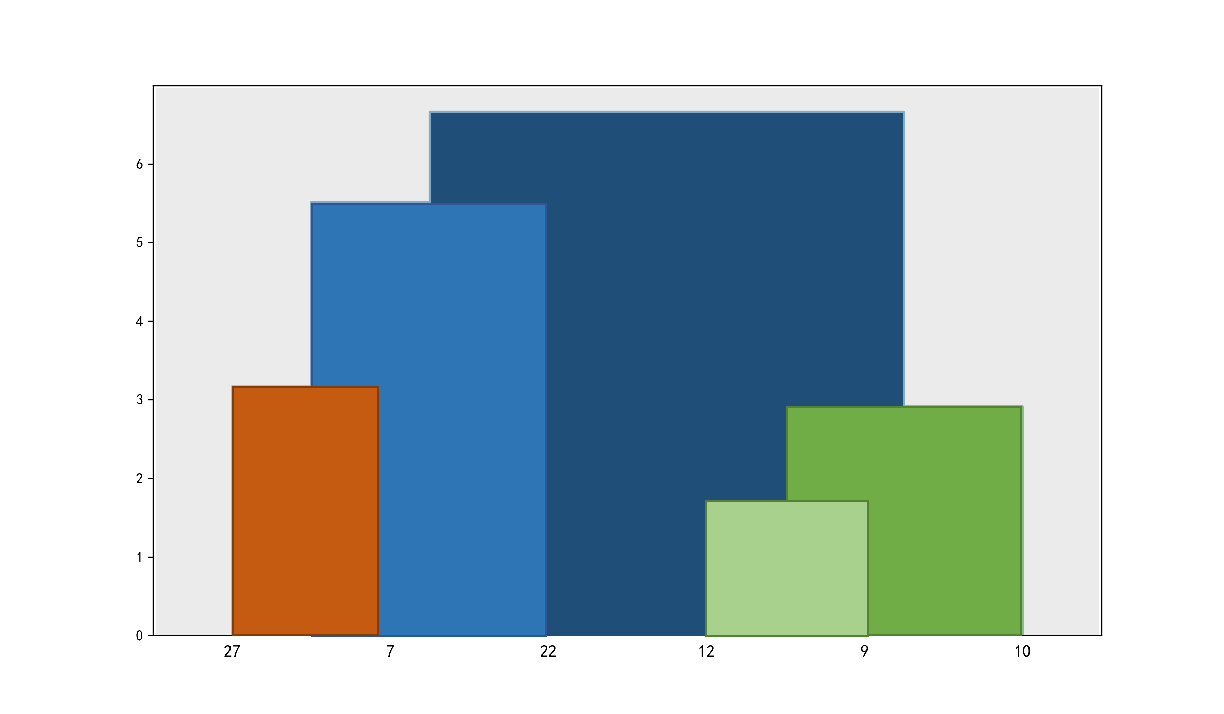
\includegraphics[width=\linewidth]{figs/4问题二/高钾玻璃_层次聚类树状图.png}
        \caption{高钾玻璃层次聚类树状图}
        \label{fig:hclust_k}
    \end{minipage}\hfill
    \begin{minipage}{0.48\textwidth}
        \centering
        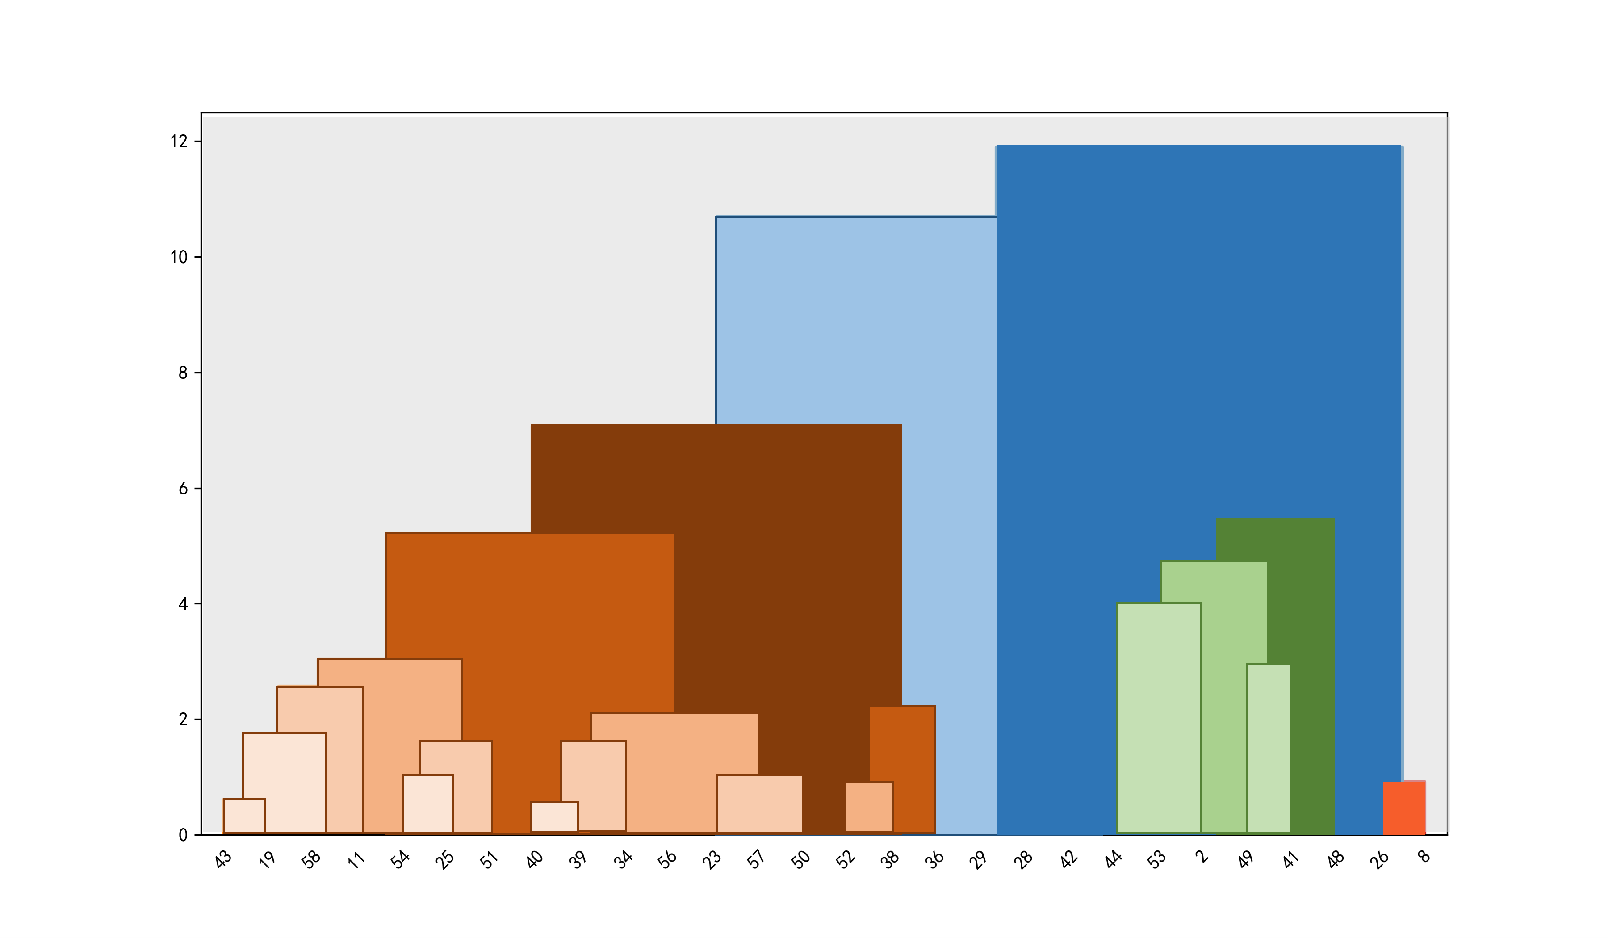
\includegraphics[width=\linewidth]{figs/4问题二/铅钡玻璃_层次聚类树状图.png}
        \caption{铅钡玻璃层次聚类树状图}
        \label{fig:hclust_pb}
    \end{minipage}
\end{figure}

图\ref{fig:hclust_pb}展示的铅钡玻璃树状图呈现出清晰的两分支结构,两个主分支在较高的距离水平上才发生合并,这初步表明铅钡玻璃样本可自然地分为两个大类。相比之下,图\ref{fig:hclust_k}中高钾玻璃的树状图结构更为复杂,呈现出多层次的嵌套聚合模式,表示其内部可能存在更多数量的亚类。

为对亚类数量的选择提供定量依据,我们引入轮廓系数指标。该指标综合评估每个样本与其所属簇的相似度即内聚性,以及与其他簇的差异度即分离度。轮廓系数值越接近一,表示聚类结果的结构越合理。

\begin{figure}[H]
    \centering
    \begin{minipage}{0.48\textwidth}
        \centering
        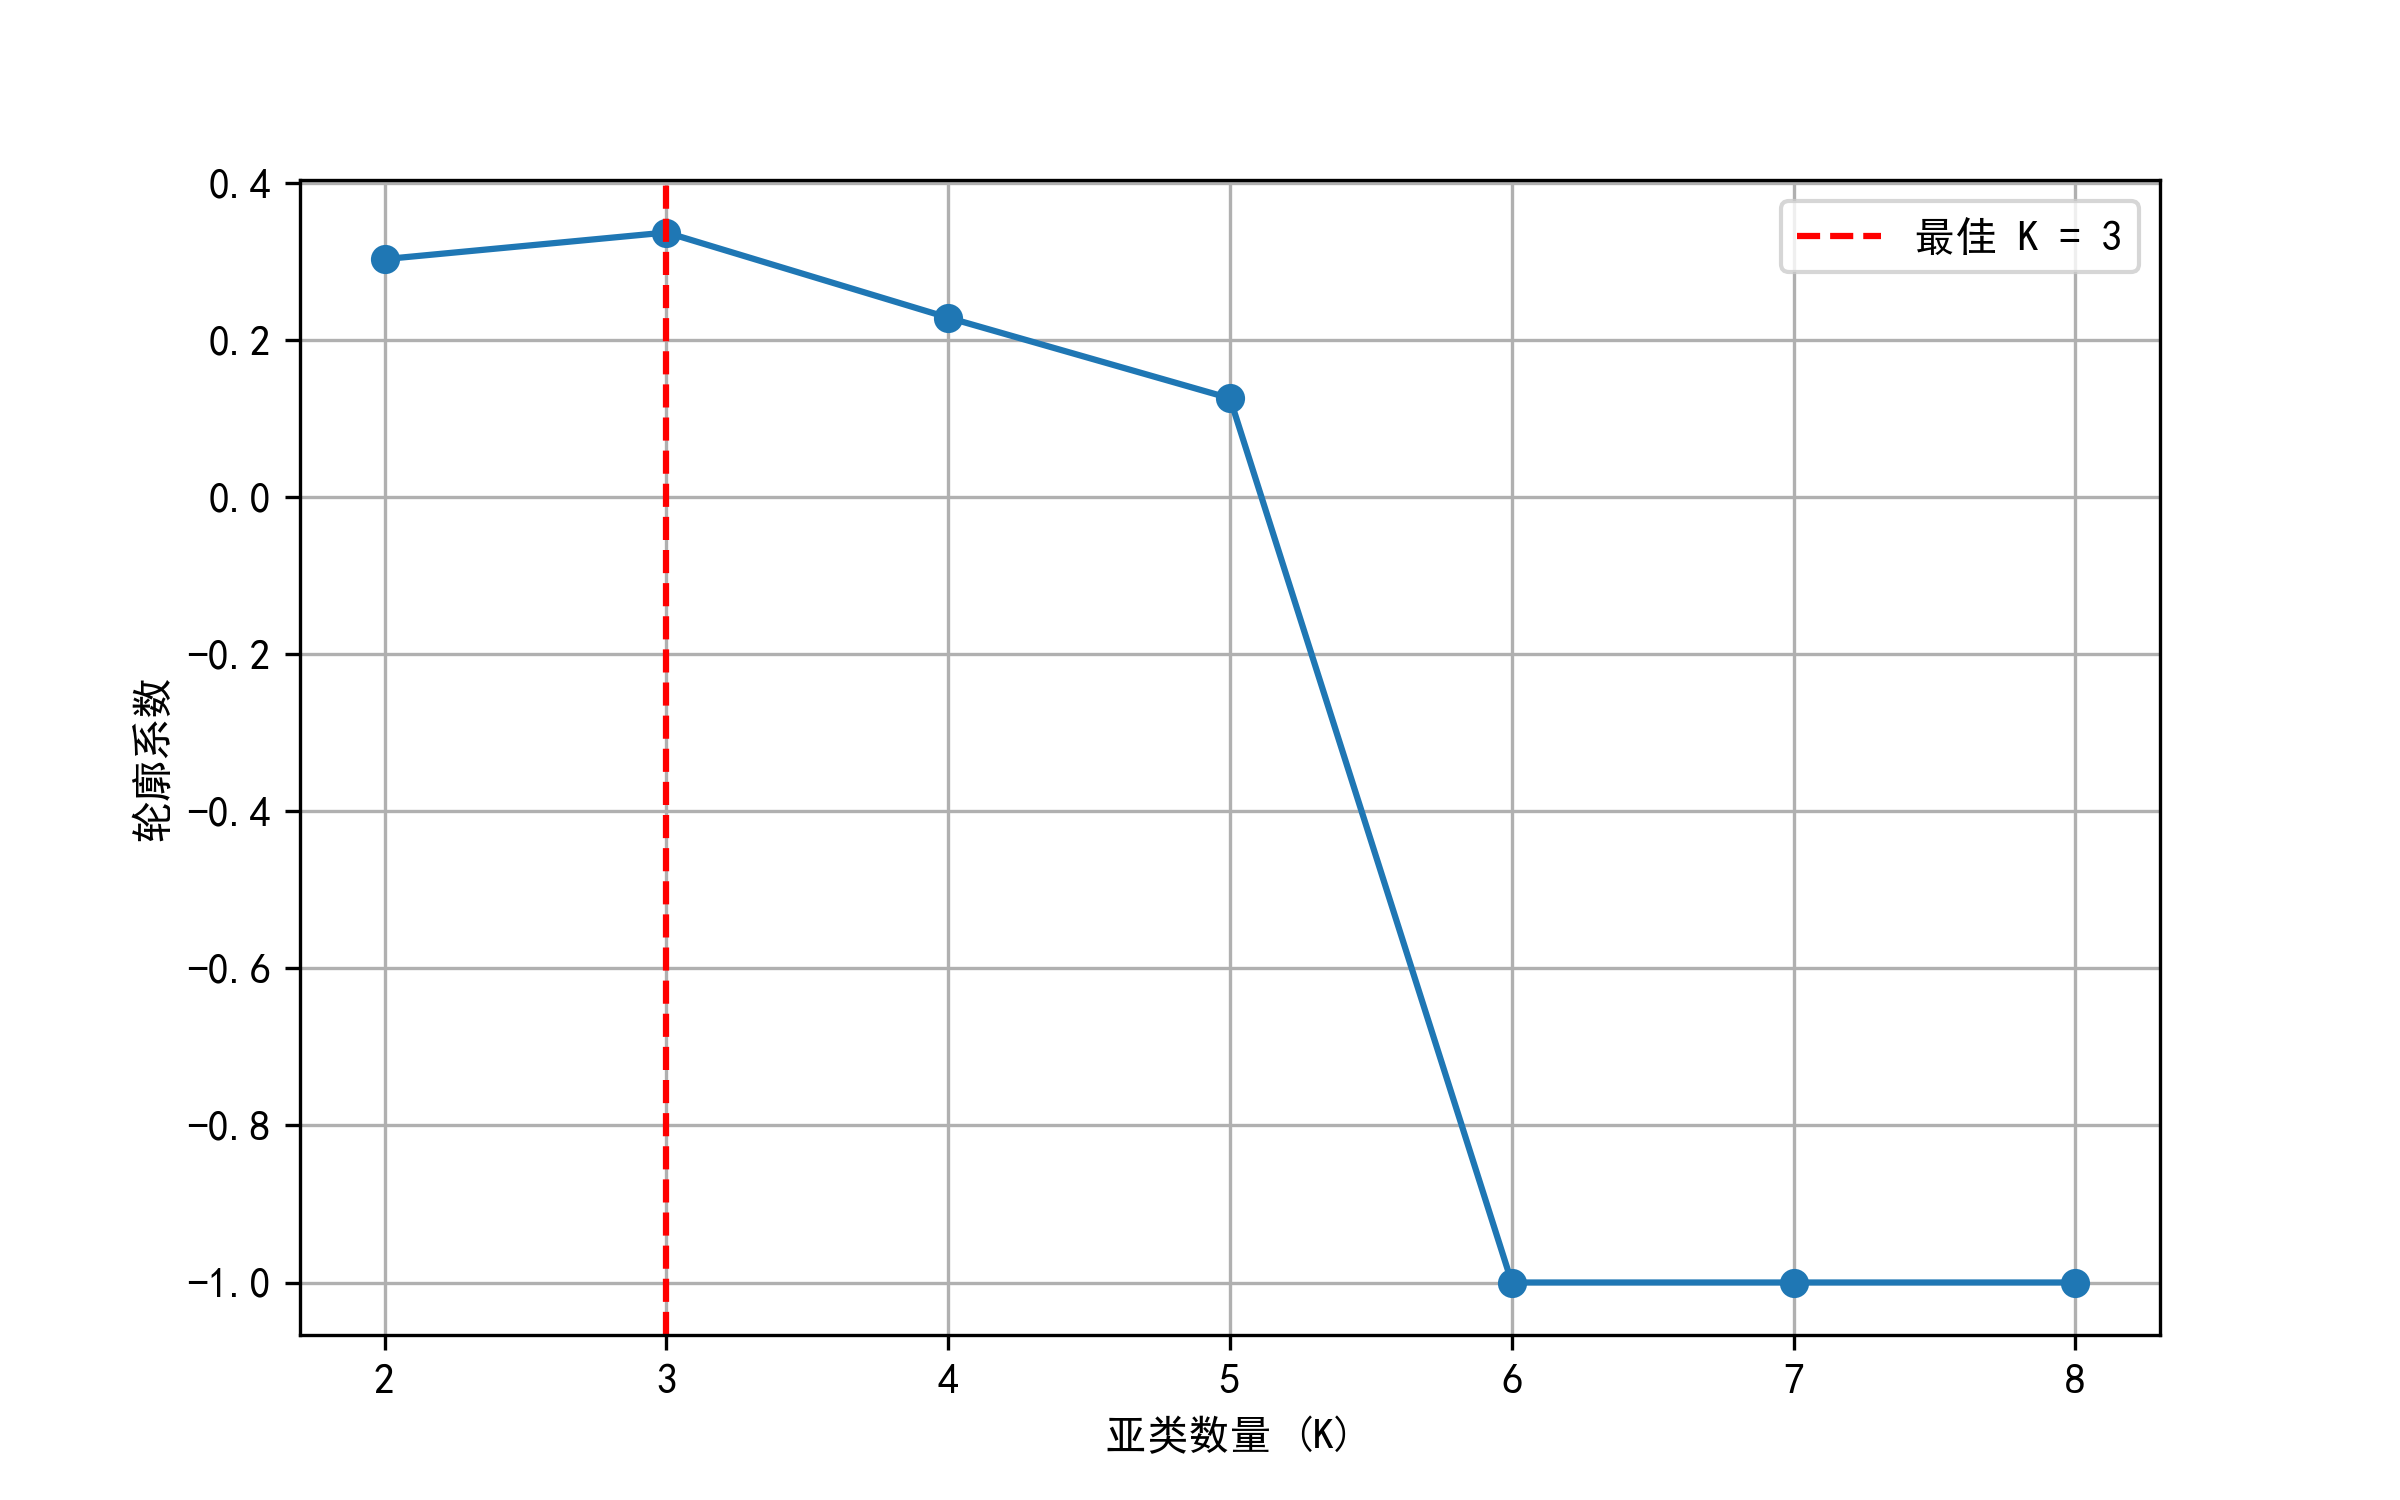
\includegraphics[width=\linewidth]{figs/4问题二/高钾玻璃_最佳K值选择.png}
        \caption{高钾玻璃轮廓系数随K值的变化}
        \label{fig:k_select_k}
    \end{minipage}\hfill
    \begin{minipage}{0.48\textwidth}
        \centering
        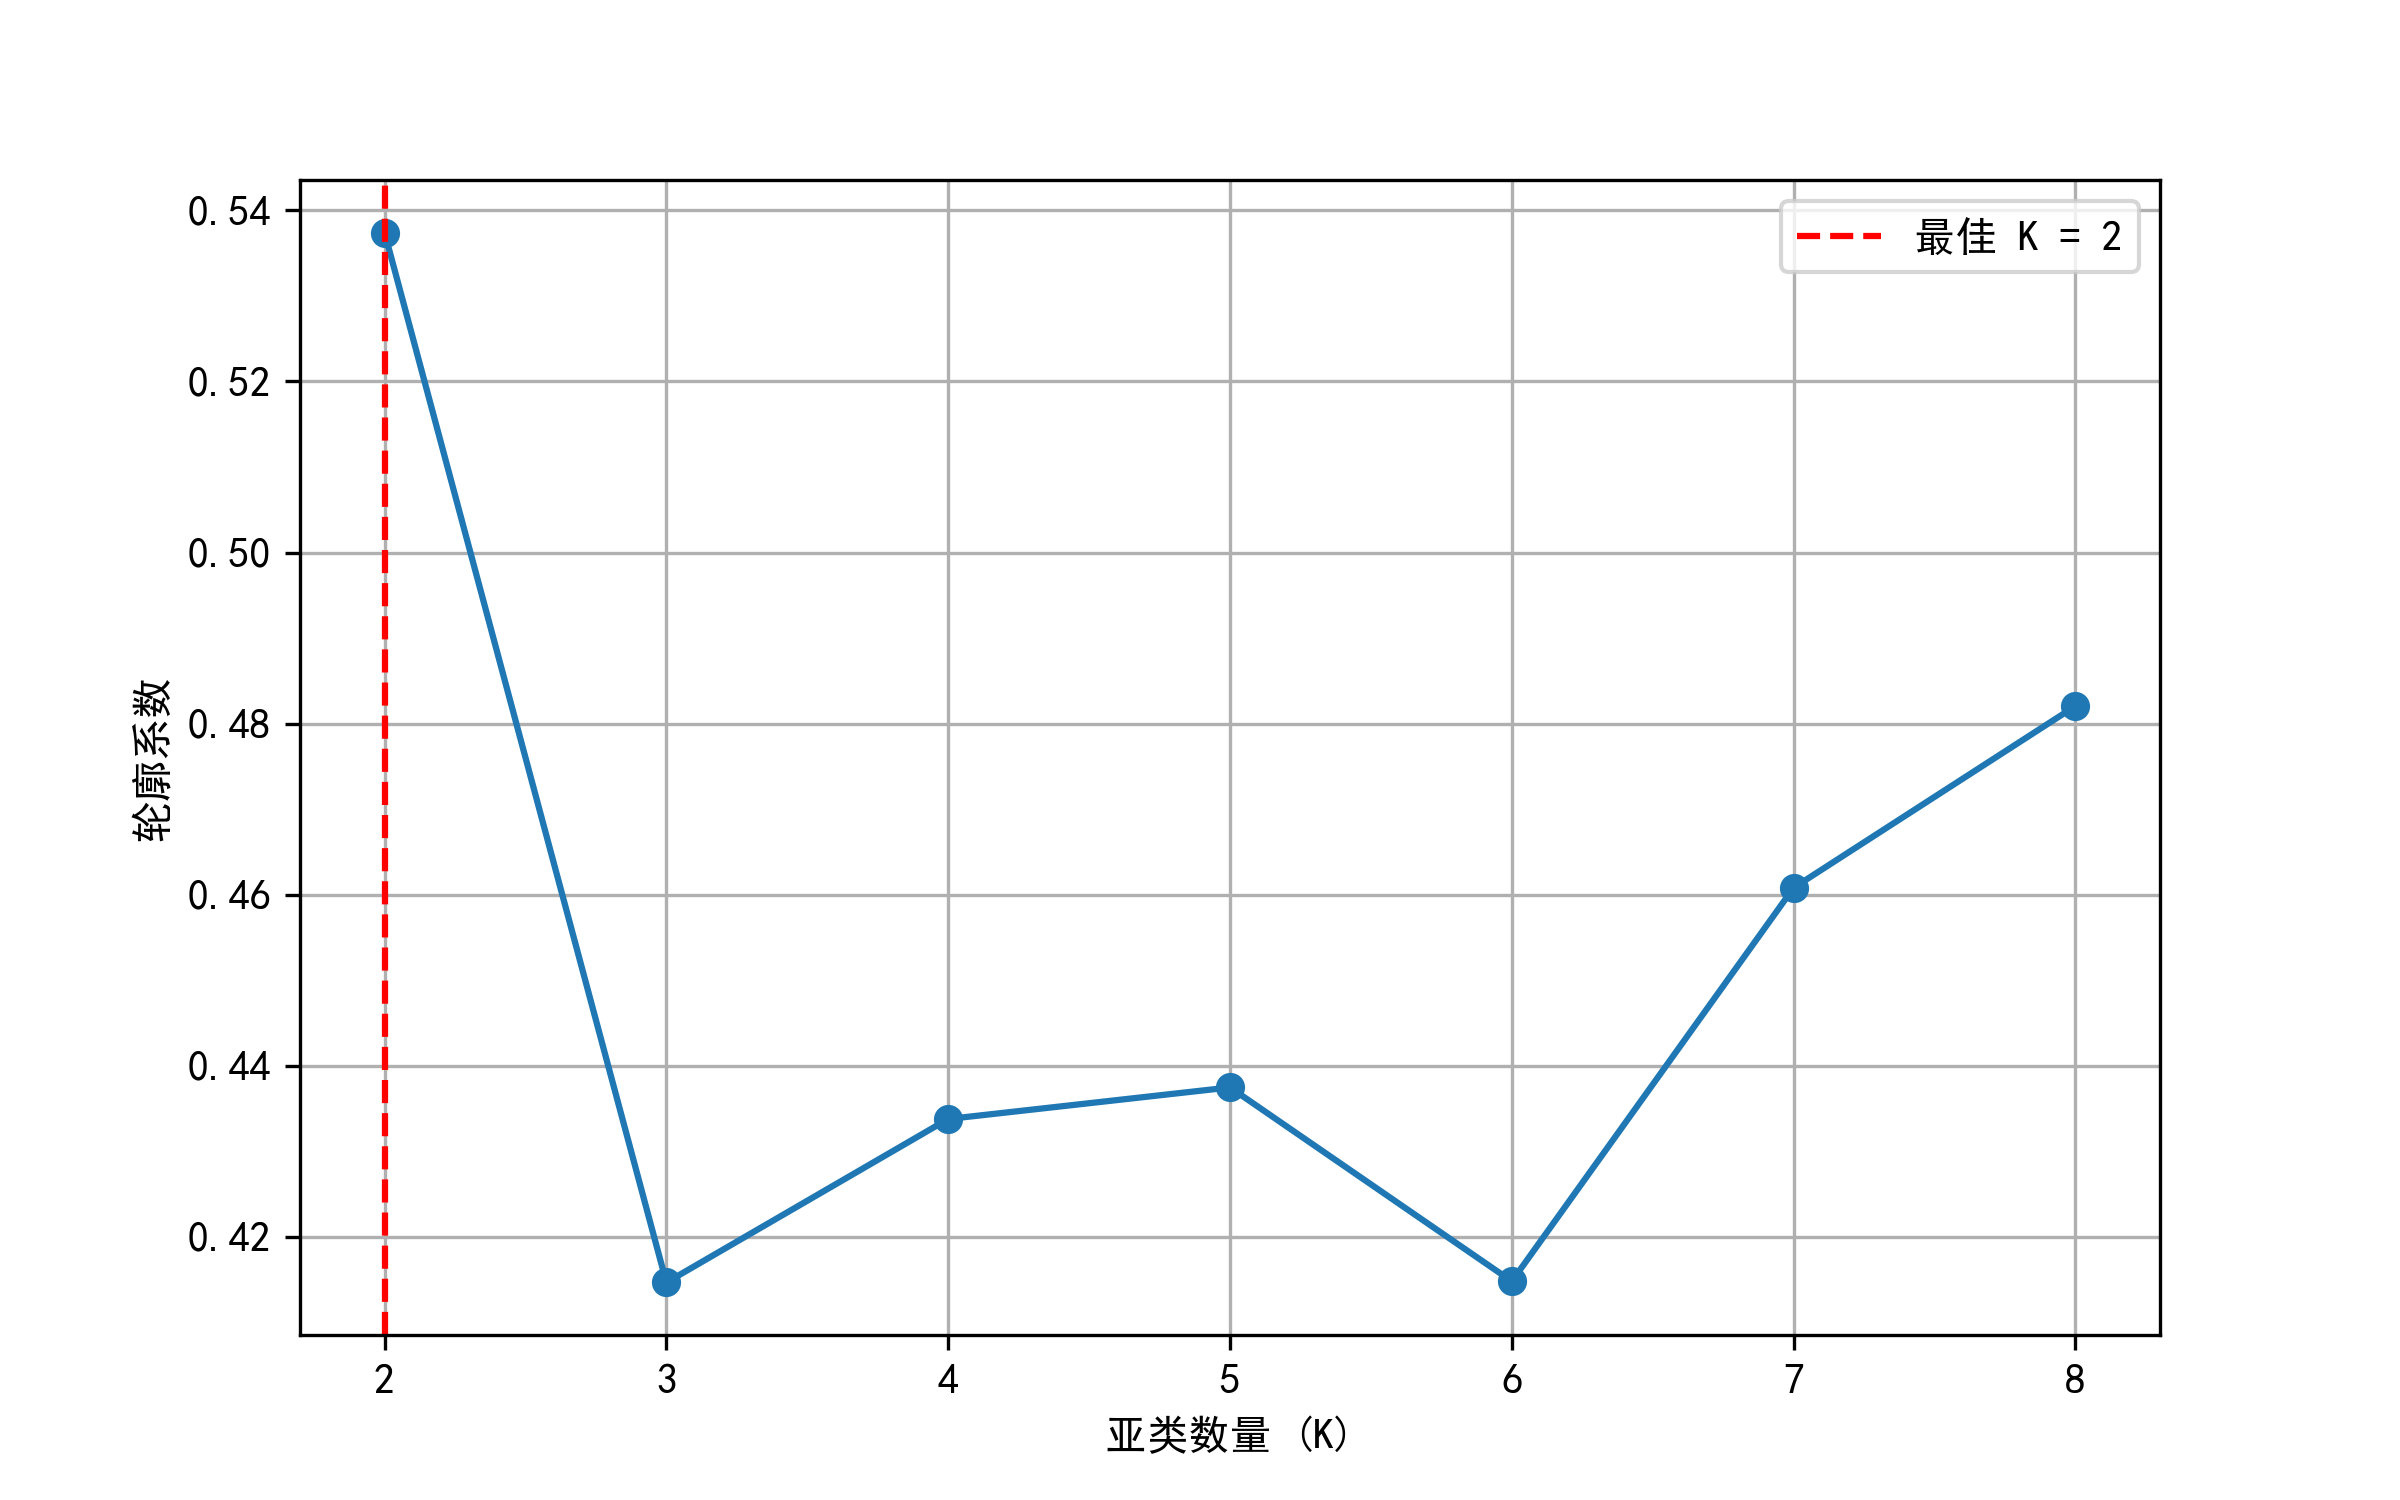
\includegraphics[width=\linewidth]{figs/4问题二/铅钡玻璃_最佳K值选择.png}
        \caption{铅钡玻璃轮廓系数随K值的变化}
        \label{fig:k_select_pb}
    \end{minipage}
\end{figure}

如图\ref{fig:k_select_pb}所示,对于铅钡玻璃,轮廓系数在$K=2$时取得最大值,约为零点四八,当$K$值继续增加时,系数值出现明显下降。对于高钾玻璃,如图\ref{fig:k_select_k}所示,轮廓系数在$K=5$时达到峰值,约为零点五二。综合定性观察与定量计算,我们将铅钡玻璃的亚类数量确定为二,高钾玻璃的亚类数量确定为五。

为验证划分结果的有效性并解读各亚类的化学特征,我们首先利用主成分分析方法将高维的化学成分数据投影到二维平面上。

\begin{figure}[H]
    \centering
    \begin{minipage}{0.48\textwidth}
        \centering
        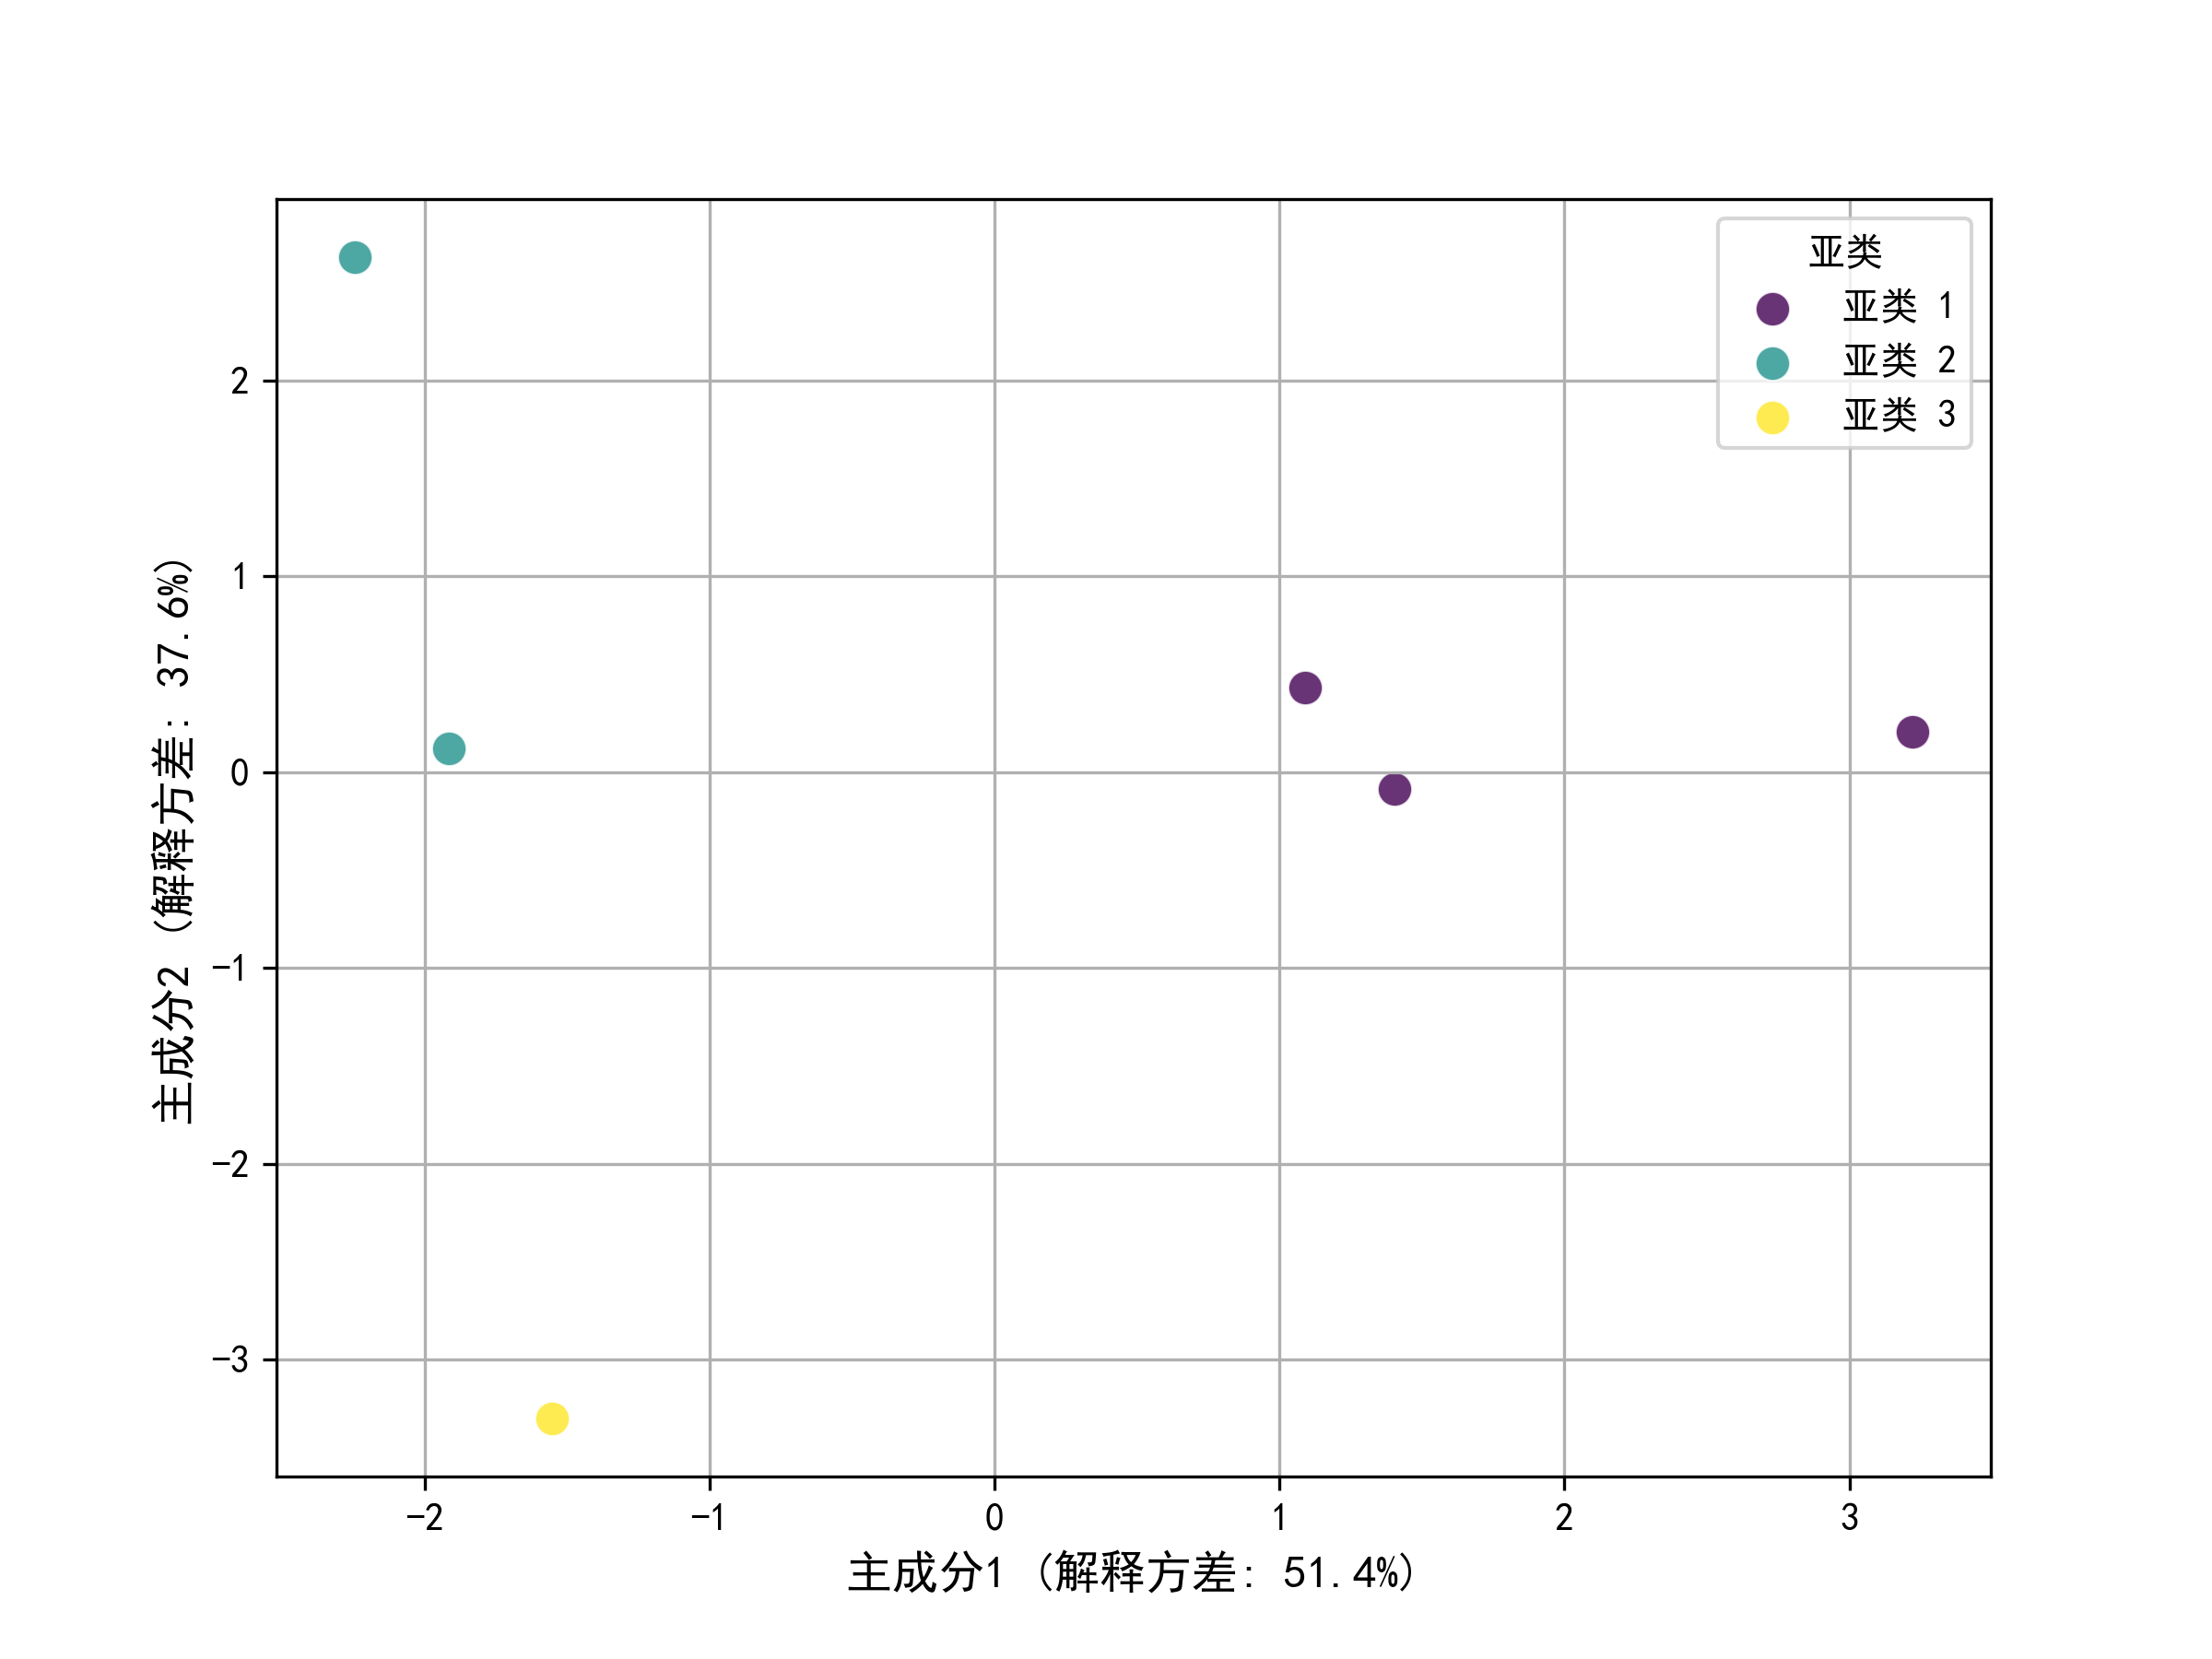
\includegraphics[width=\linewidth]{figs/4问题二/高钾玻璃_亚类PCA图.png}
        \caption{高钾玻璃亚类划分PCA可视化}
        \label{fig:pca_k}
    \end{minipage}\hfill
    \begin{minipage}{0.48\textwidth}
        \centering
        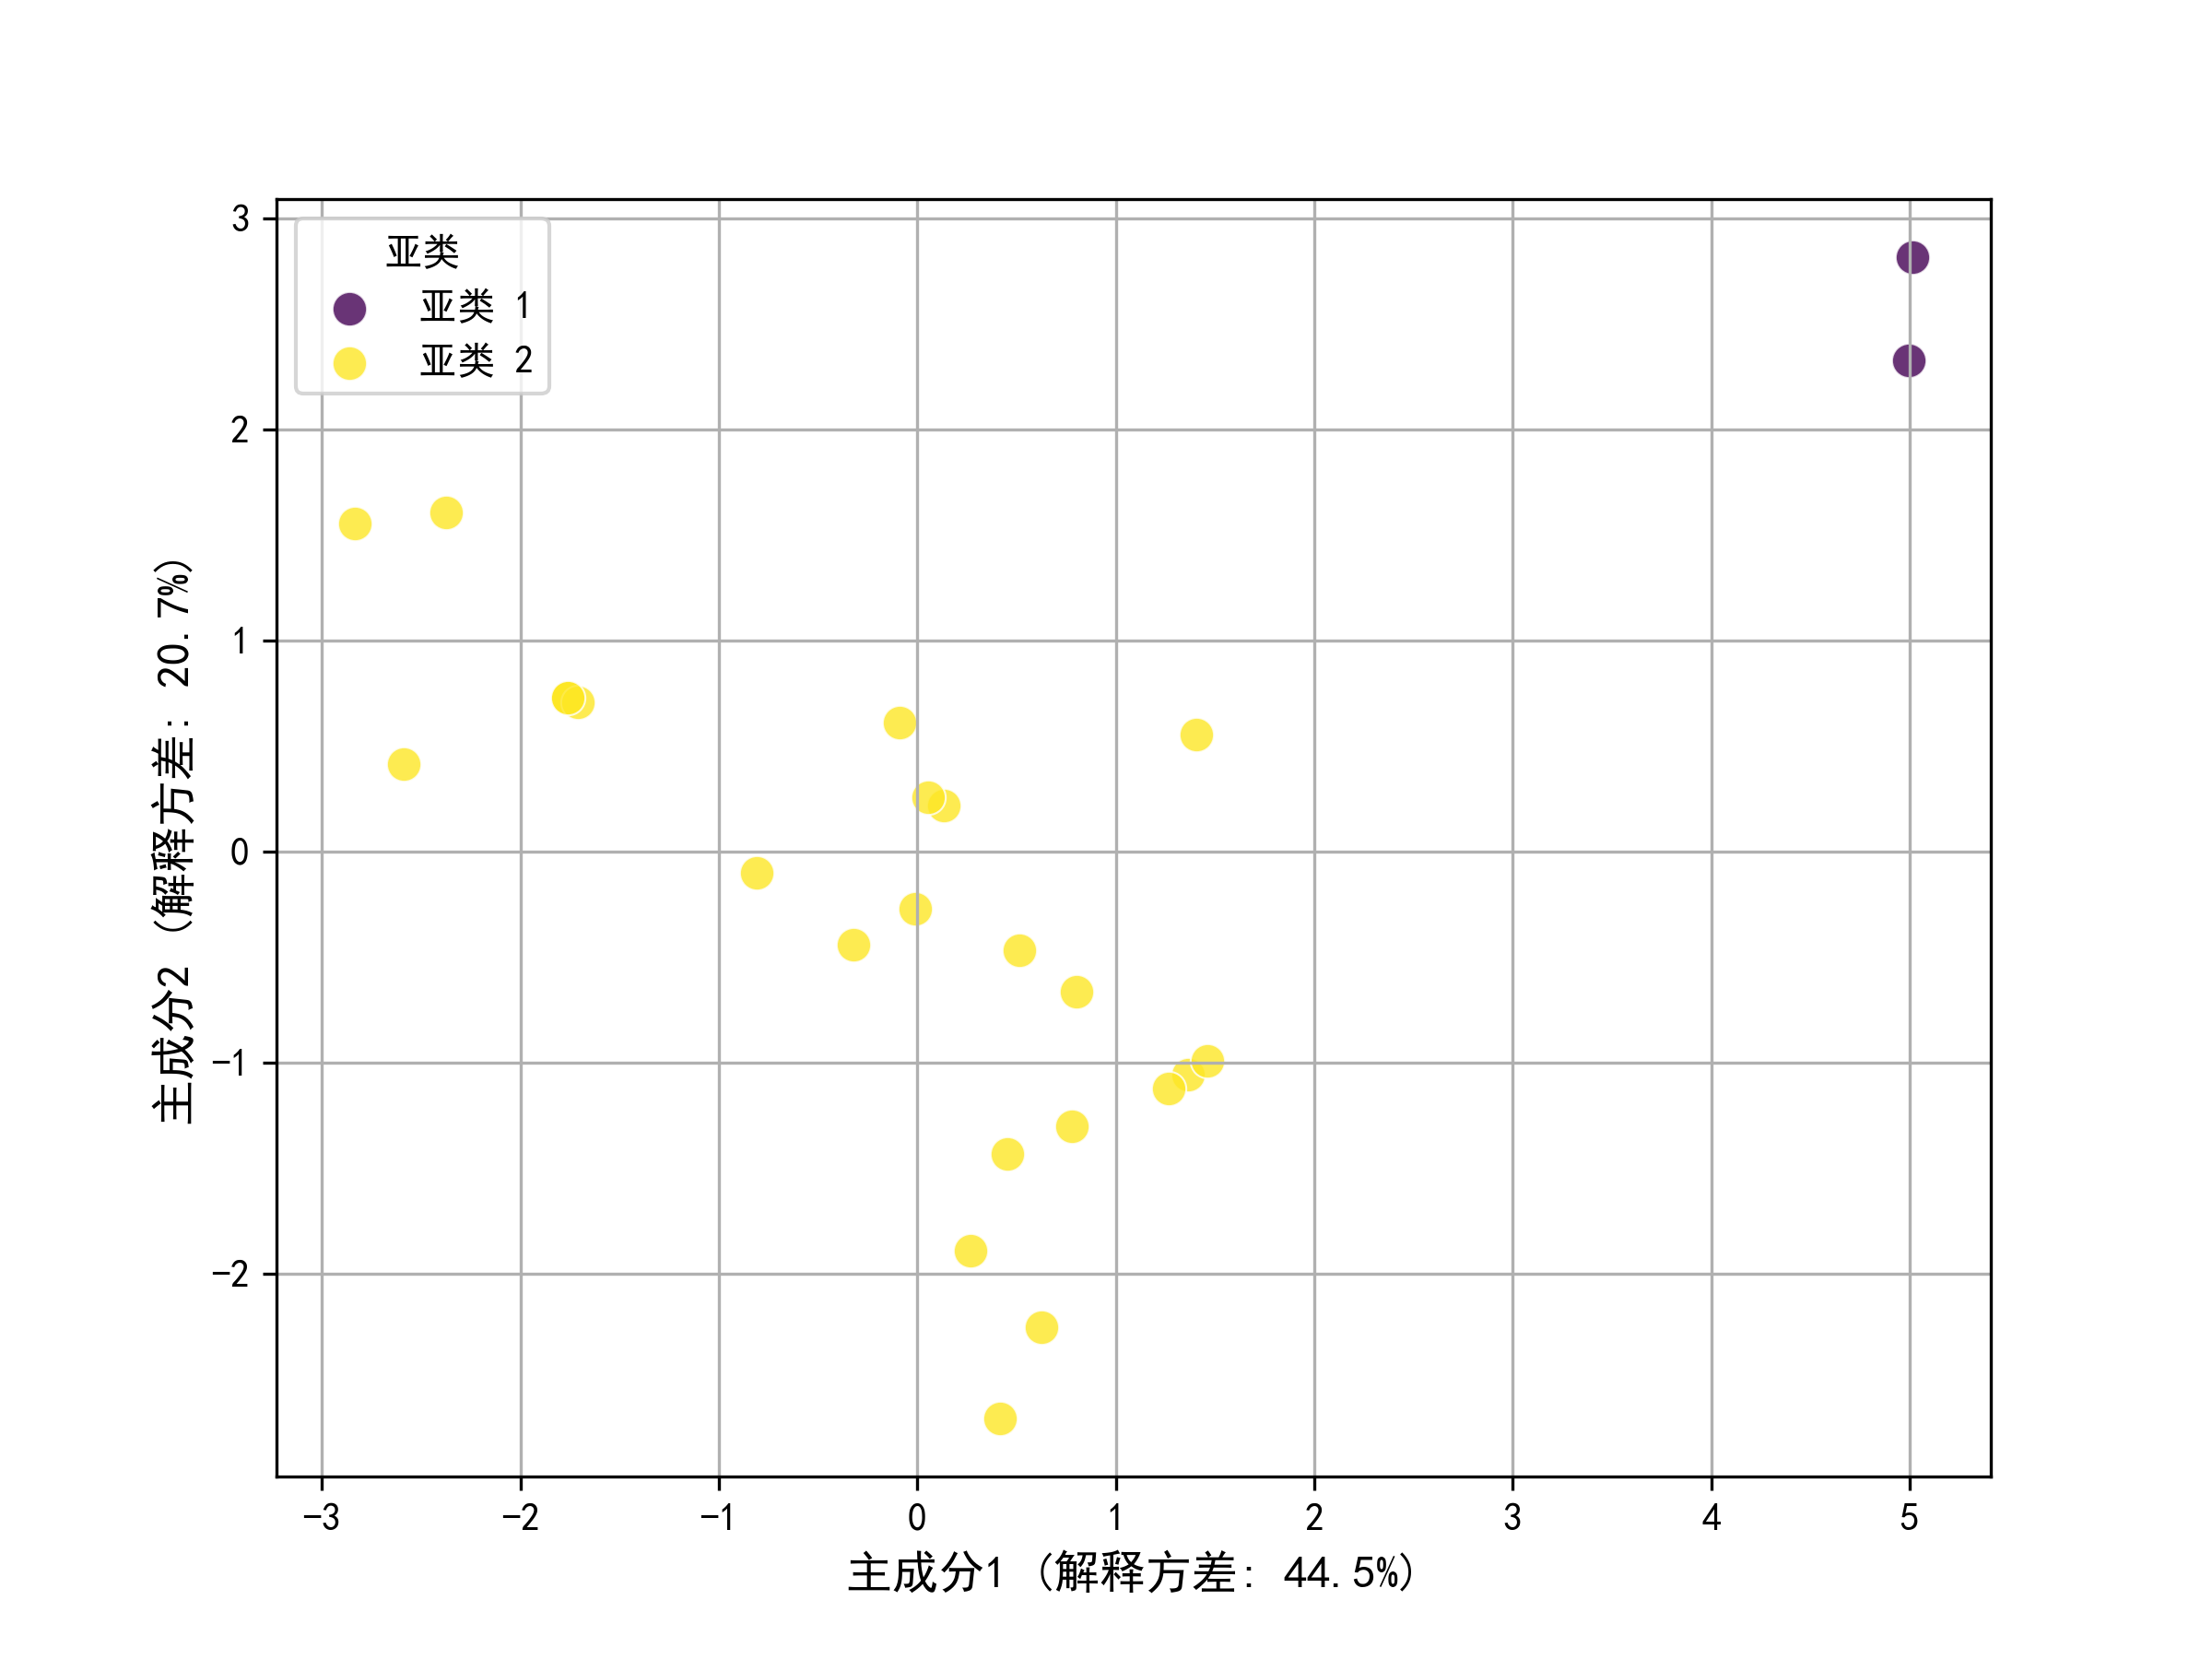
\includegraphics[width=\linewidth]{figs/4问题二/铅钡玻璃_亚类PCA图.png}
        \caption{铅钡玻璃亚类划分PCA可视化}
        \label{fig:pca_pb}
    \end{minipage}
\end{figure}

图\ref{fig:pca_k}与图\ref{fig:pca_pb}的可视化结果显示,不同颜色的点代表不同亚类的样本。铅钡玻璃的两个亚类在第一主成分轴上具有显著的分离。高钾玻璃的五个亚类也在二维空间中占据了相对独立的区域,各亚类内部样本较为集中,而亚类之间存在明显界限。

为进一步阐释每个亚类所代表的化学成分模式,我们绘制了亚类化学特征热力图。

\begin{figure}[H]
    \centering
    \begin{minipage}{0.48\textwidth}
        \centering
        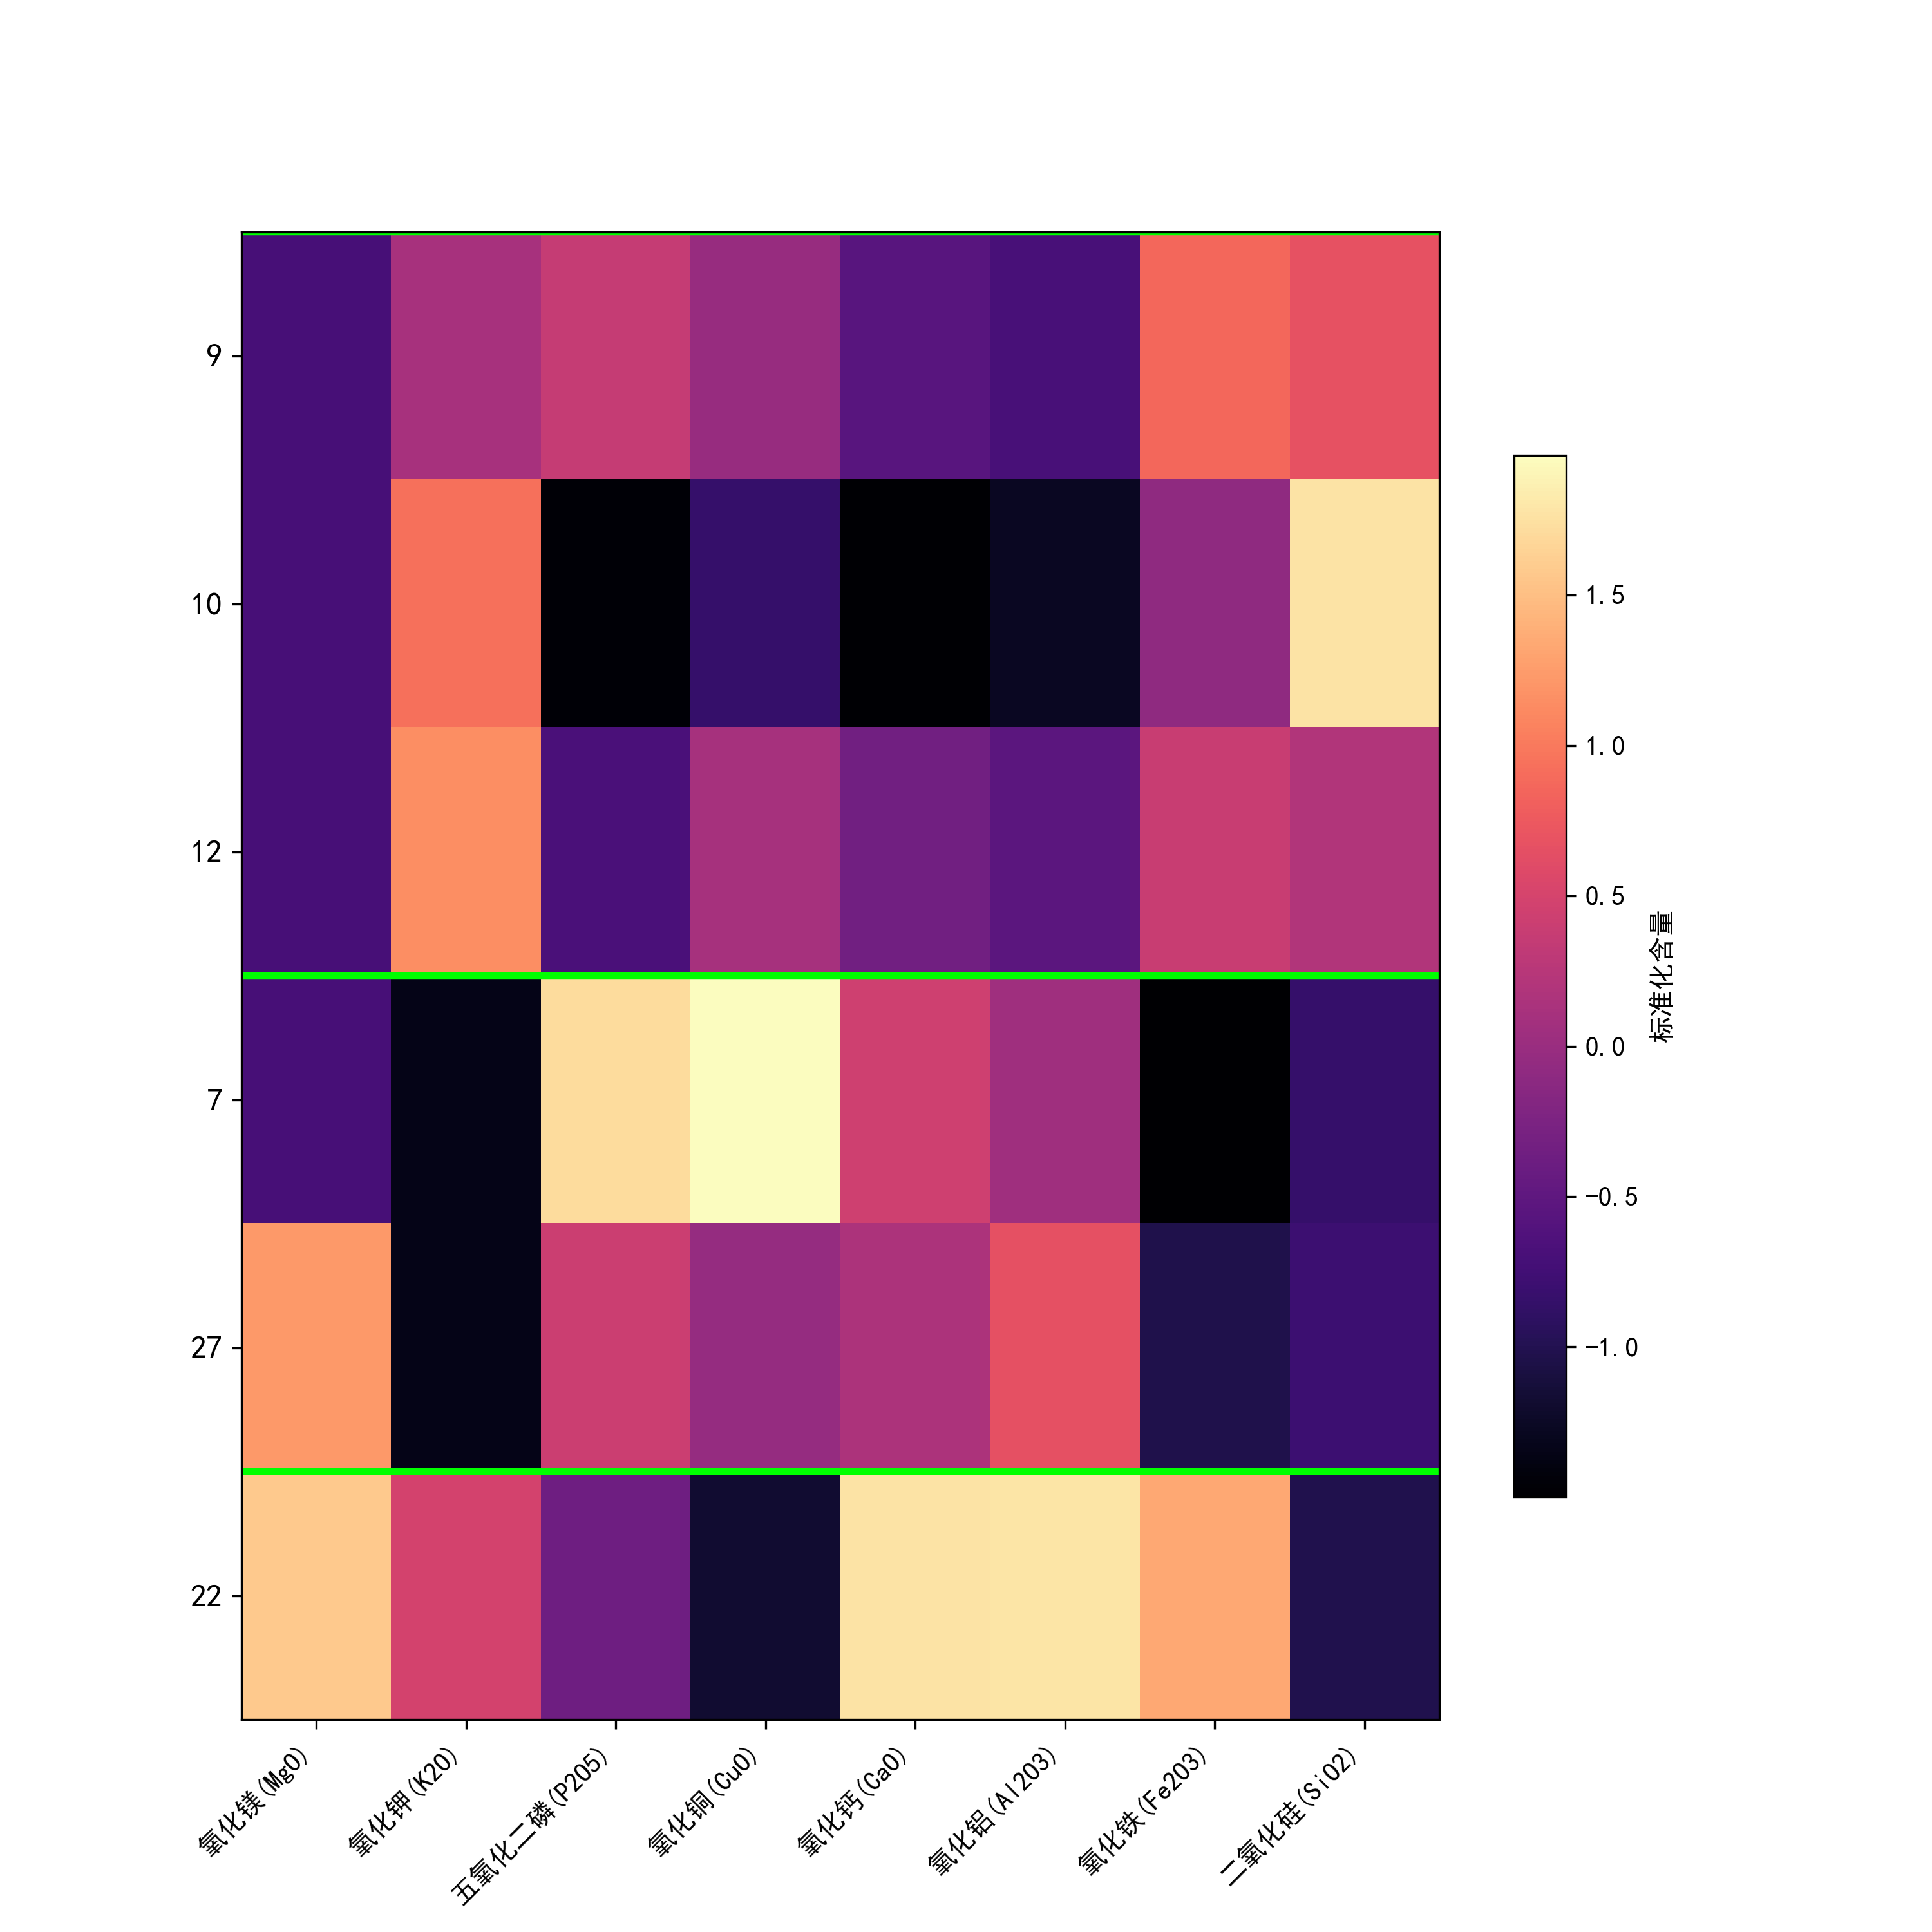
\includegraphics[width=\linewidth]{figs/4问题二/高钾玻璃_亚类热力图_带编号.png}
        \caption{高钾玻璃亚类化学特征热力图}
        \label{fig:heatmap_k}
    \end{minipage}\hfill
    \begin{minipage}{0.48\textwidth}
        \centering
        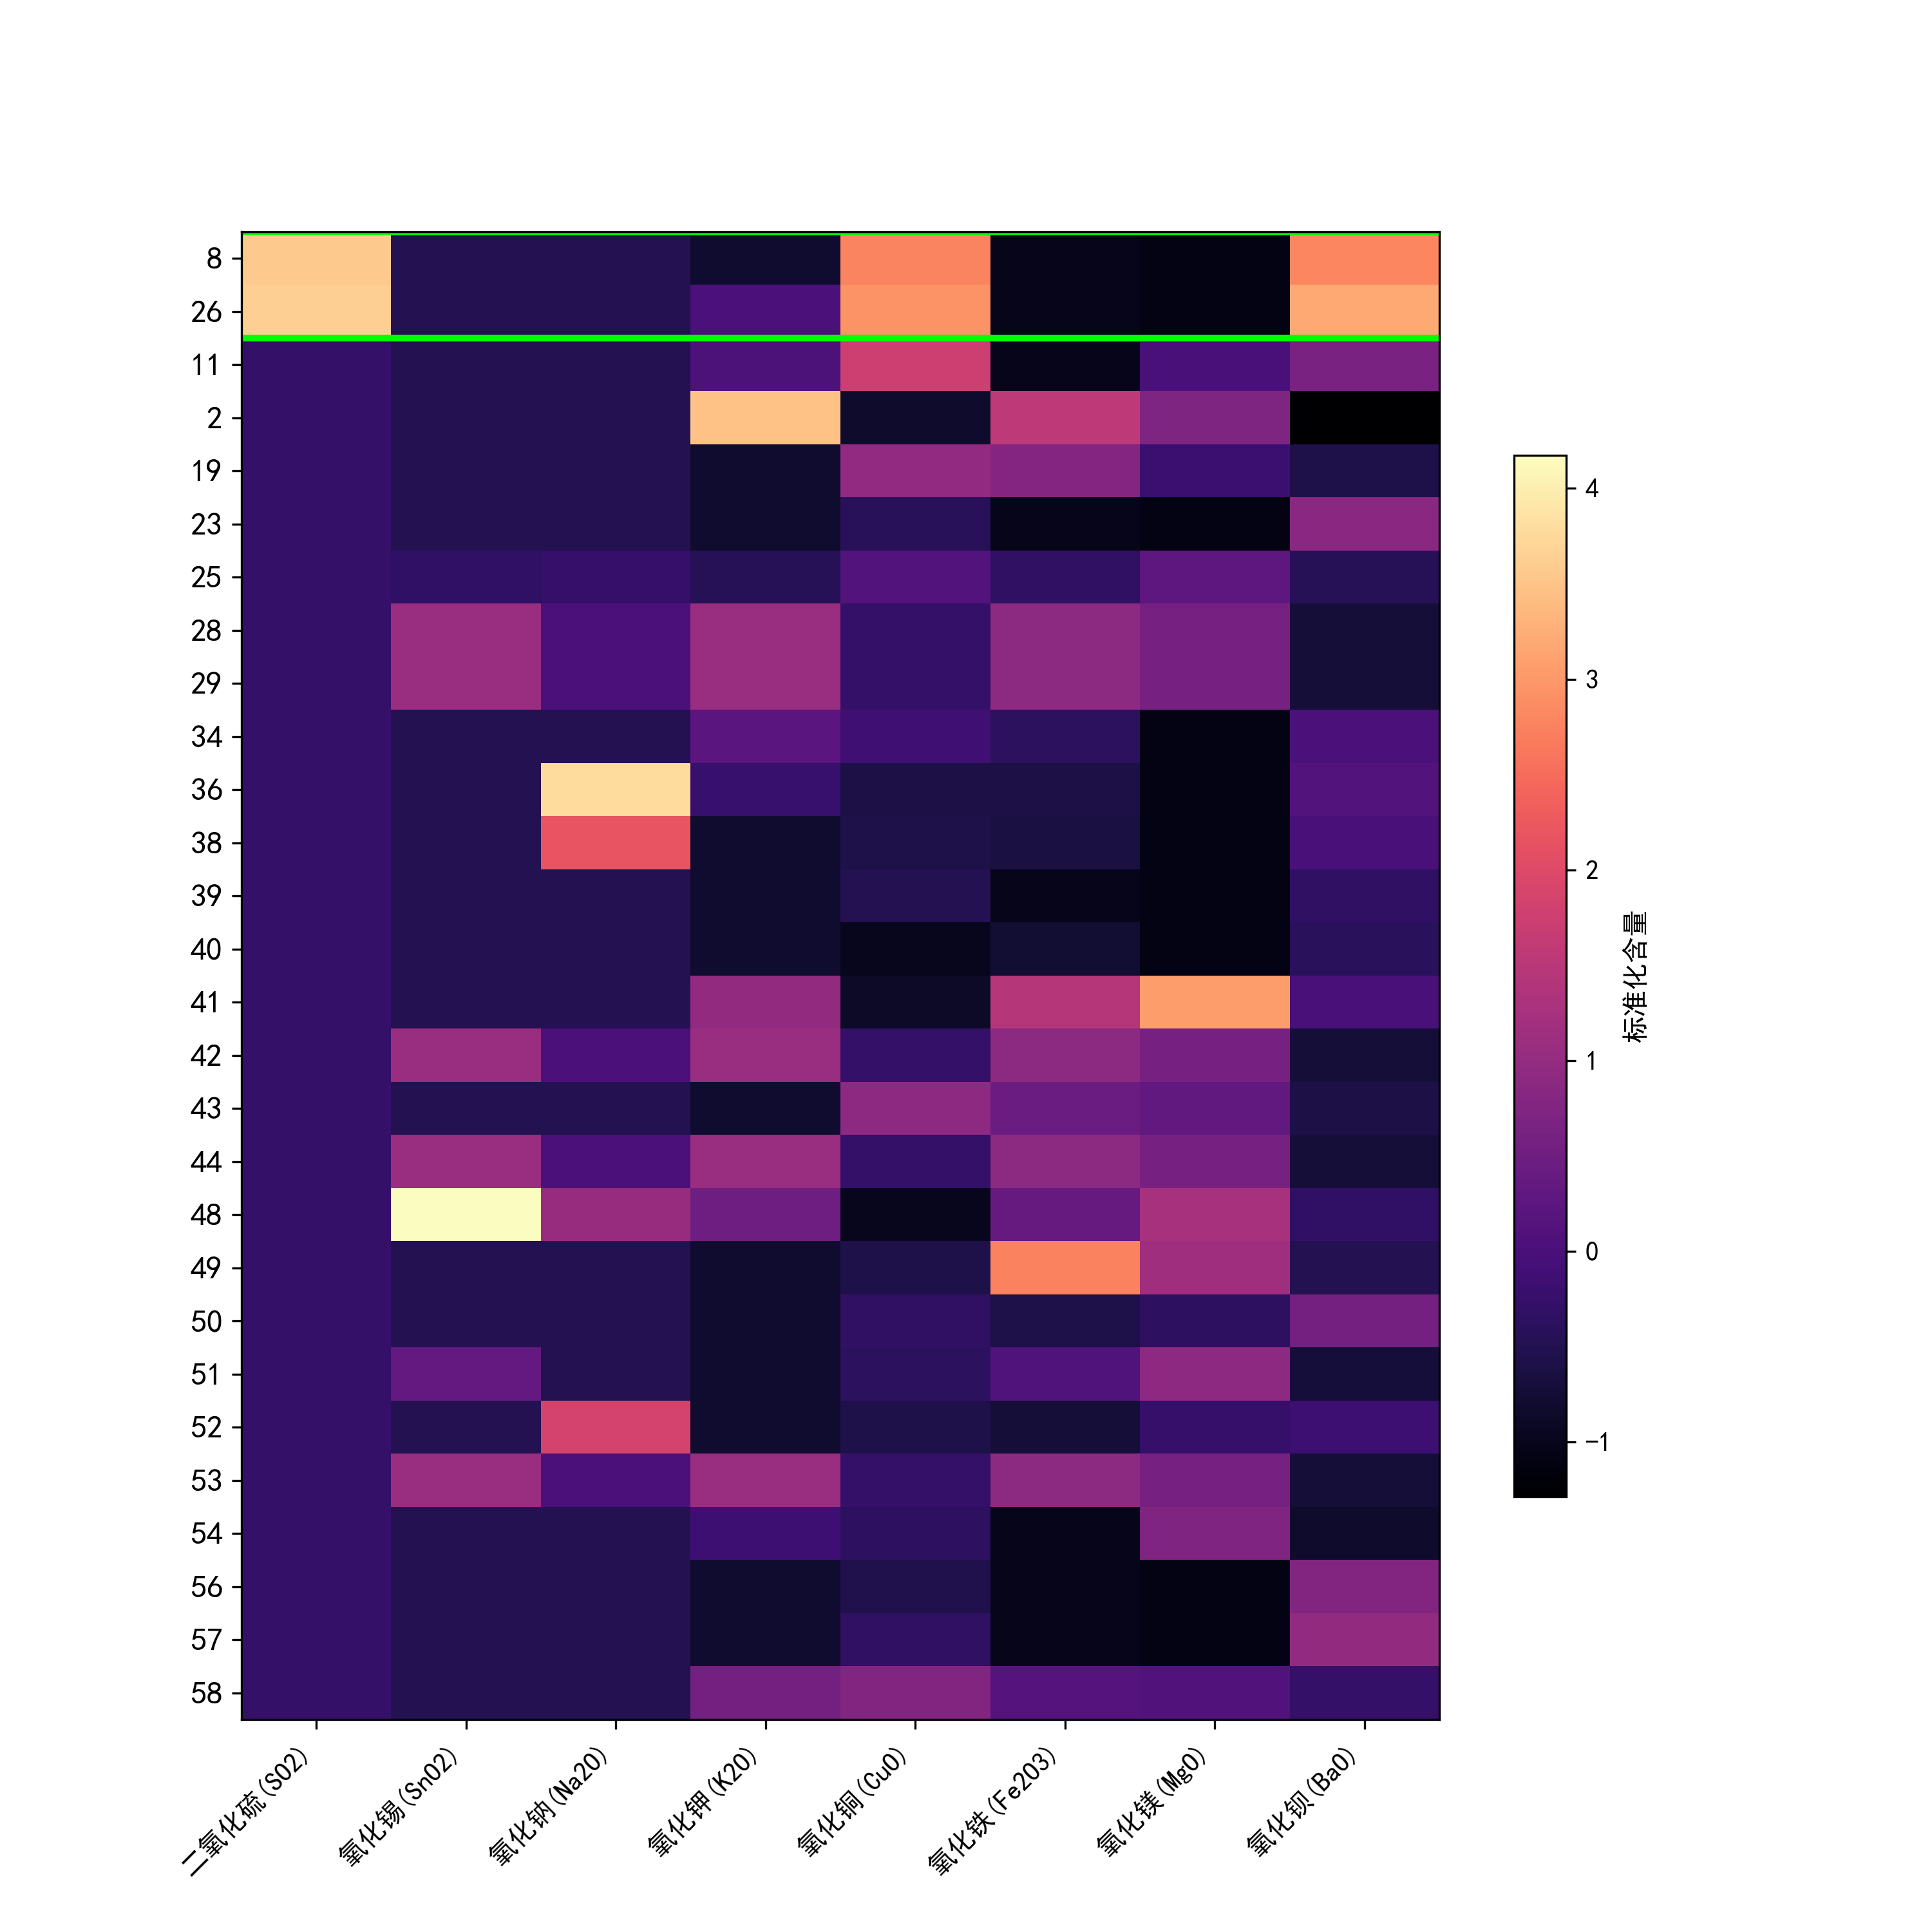
\includegraphics[width=\linewidth]{figs/4问题二/铅钡玻璃_亚类热力图_带编号.png}
        \caption{铅钡玻璃亚类化学特征热力图}
        \label{fig:heatmap_pb}
    \end{minipage}
\end{figure}

图\ref{fig:heatmap_pb}展示了铅钡玻璃两个亚类的化学差异。亚类一的样本在氧化铅$PbO$与氧化钡$BaO$两种助熔剂成分上呈现深色,表明其含量普遍较高,而作为玻璃基体的二氧化硅$SiO_2$含量则相对较低。与此相反,亚类零的样本在二氧化硅$SiO_2$上呈现深色,含量普遍较高,而氧化铅$PbO$与氧化钡$BaO$含量则较低。基于此,可将亚类一命名为高铅钡助熔剂型,亚类零命名为高硅基质型。

图\ref{fig:heatmap_k}则展现了高钾玻璃五个亚类更为细微的化学特征。亚类二的突出特征是其氧化钾$K_2O$含量极高,而其他成分含量较低。亚类一的氧化钙$CaO$含量相对突出。亚类零则表现为氧化铝$Al_2O_3$与氧化铁$Fe_2O_3$含量较高,这可能与其他亚类使用了不同的矿物原料有关。亚类三与亚类四的差异主要体现在磷与硫等微量元素上,反映了更为精细的原料或工艺差别。通过热力图分析,我们明确了每个亚类独特的化学成分特征。


\subsection{结果的敏感性分析}

为验证上述分类与划分结果的稳健性,我们进行了敏感性分析。首先,我们检验分类规律的可靠性。我们在十折交叉验证的每一次折叠中,重新训练线性支持向量机模型并提取其权重,以评估规律本身的稳定性。

\begin{figure}[H]
    \centering
    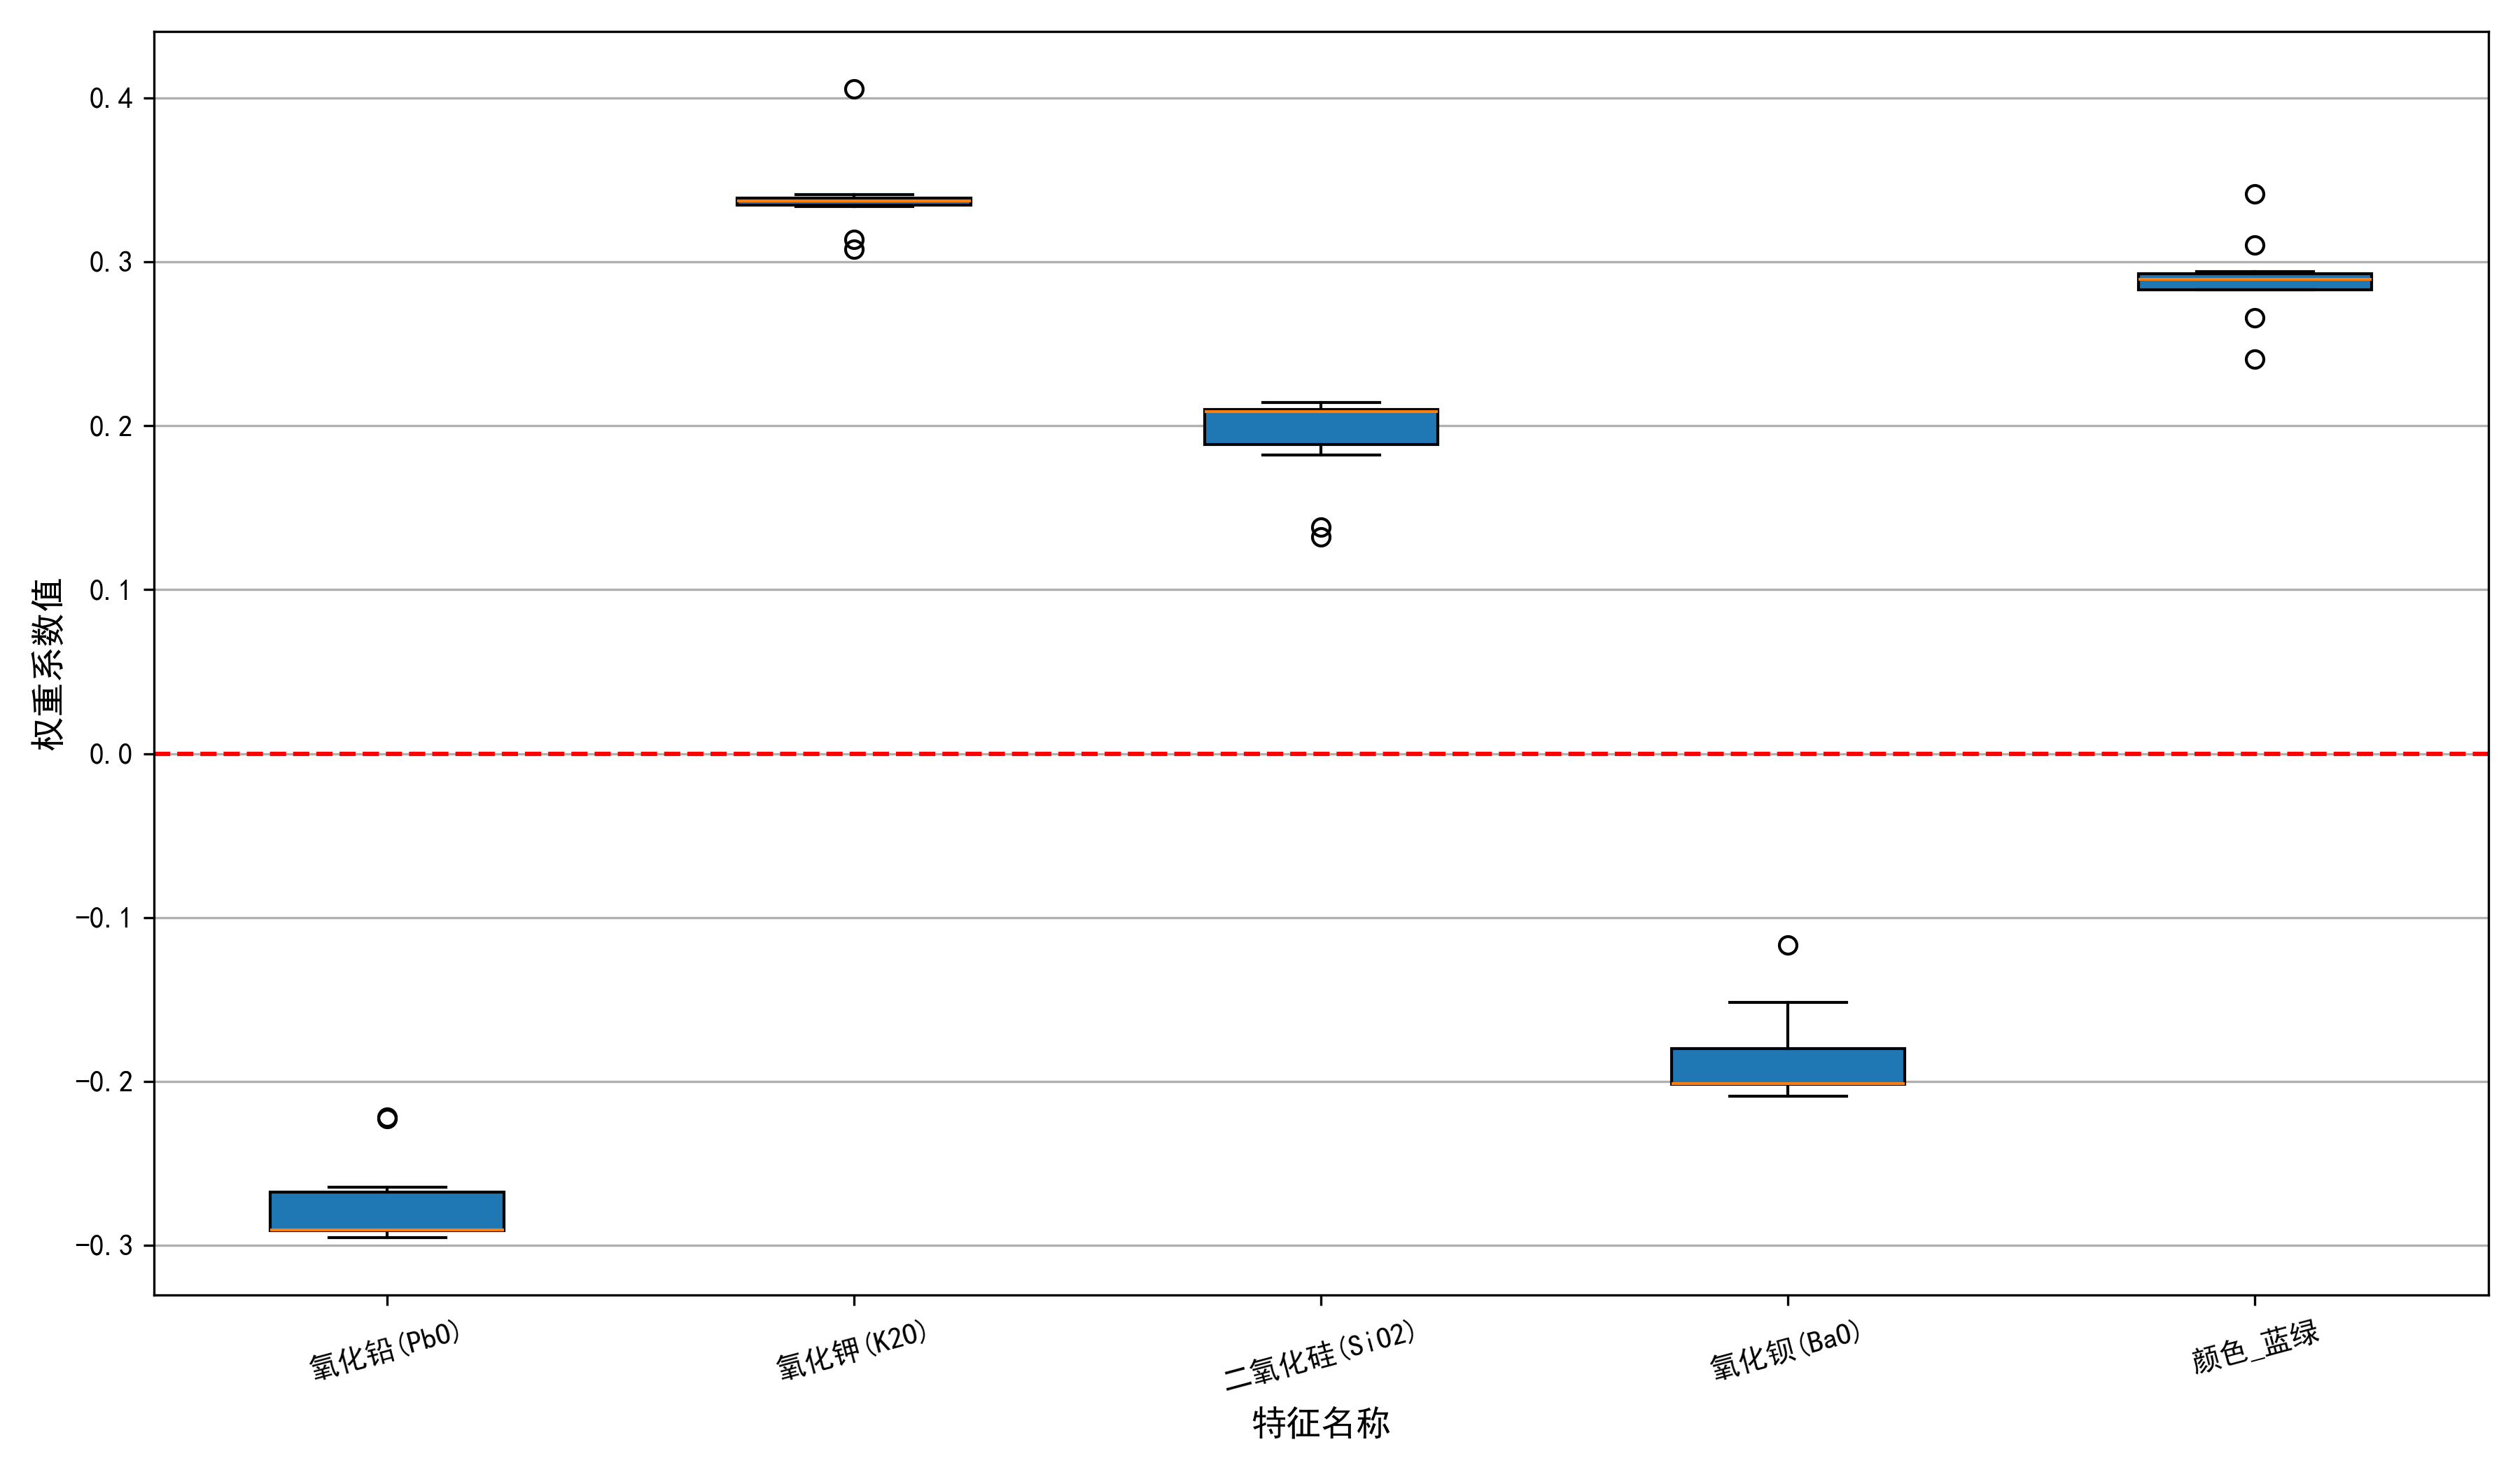
\includegraphics[width=\textwidth]{figs/4问题二/SVM权重稳定性分析.png}
    \caption{关键特征的SVM权重在十次交叉验证中的稳定性}
    \label{fig:svm_stability}
\end{figure}

图\ref{fig:svm_stability}通过箱线图展示了关键特征的权重在十次不同数据子集训练中的分布。图中显示,关键特征如$PbO$、$K_2O$的权重符号在十次实验中从未改变,且波动范围很小。这证明了我们提炼出的分类规律是高度稳健的。

其次,我们检验亚类划分结果的敏感性。为检验划分结果对化学成分测量误差的容忍度,我们采用了特征值扰动法。该方法通过向数据中注入不同水平的随机噪声,来模拟测量误差,并检验聚类结构的稳定性。我们对筛选出的特征数据乘以一个范围在$[1-p, 1+p]$内的随机扰动因子,其中$p$为扰动水平。在此扰动数据上重新聚类,并使用调整兰德指数$ARI$来衡量该次聚类结果与原始基准结果的一致性。

\begin{figure}[H]
    \centering
    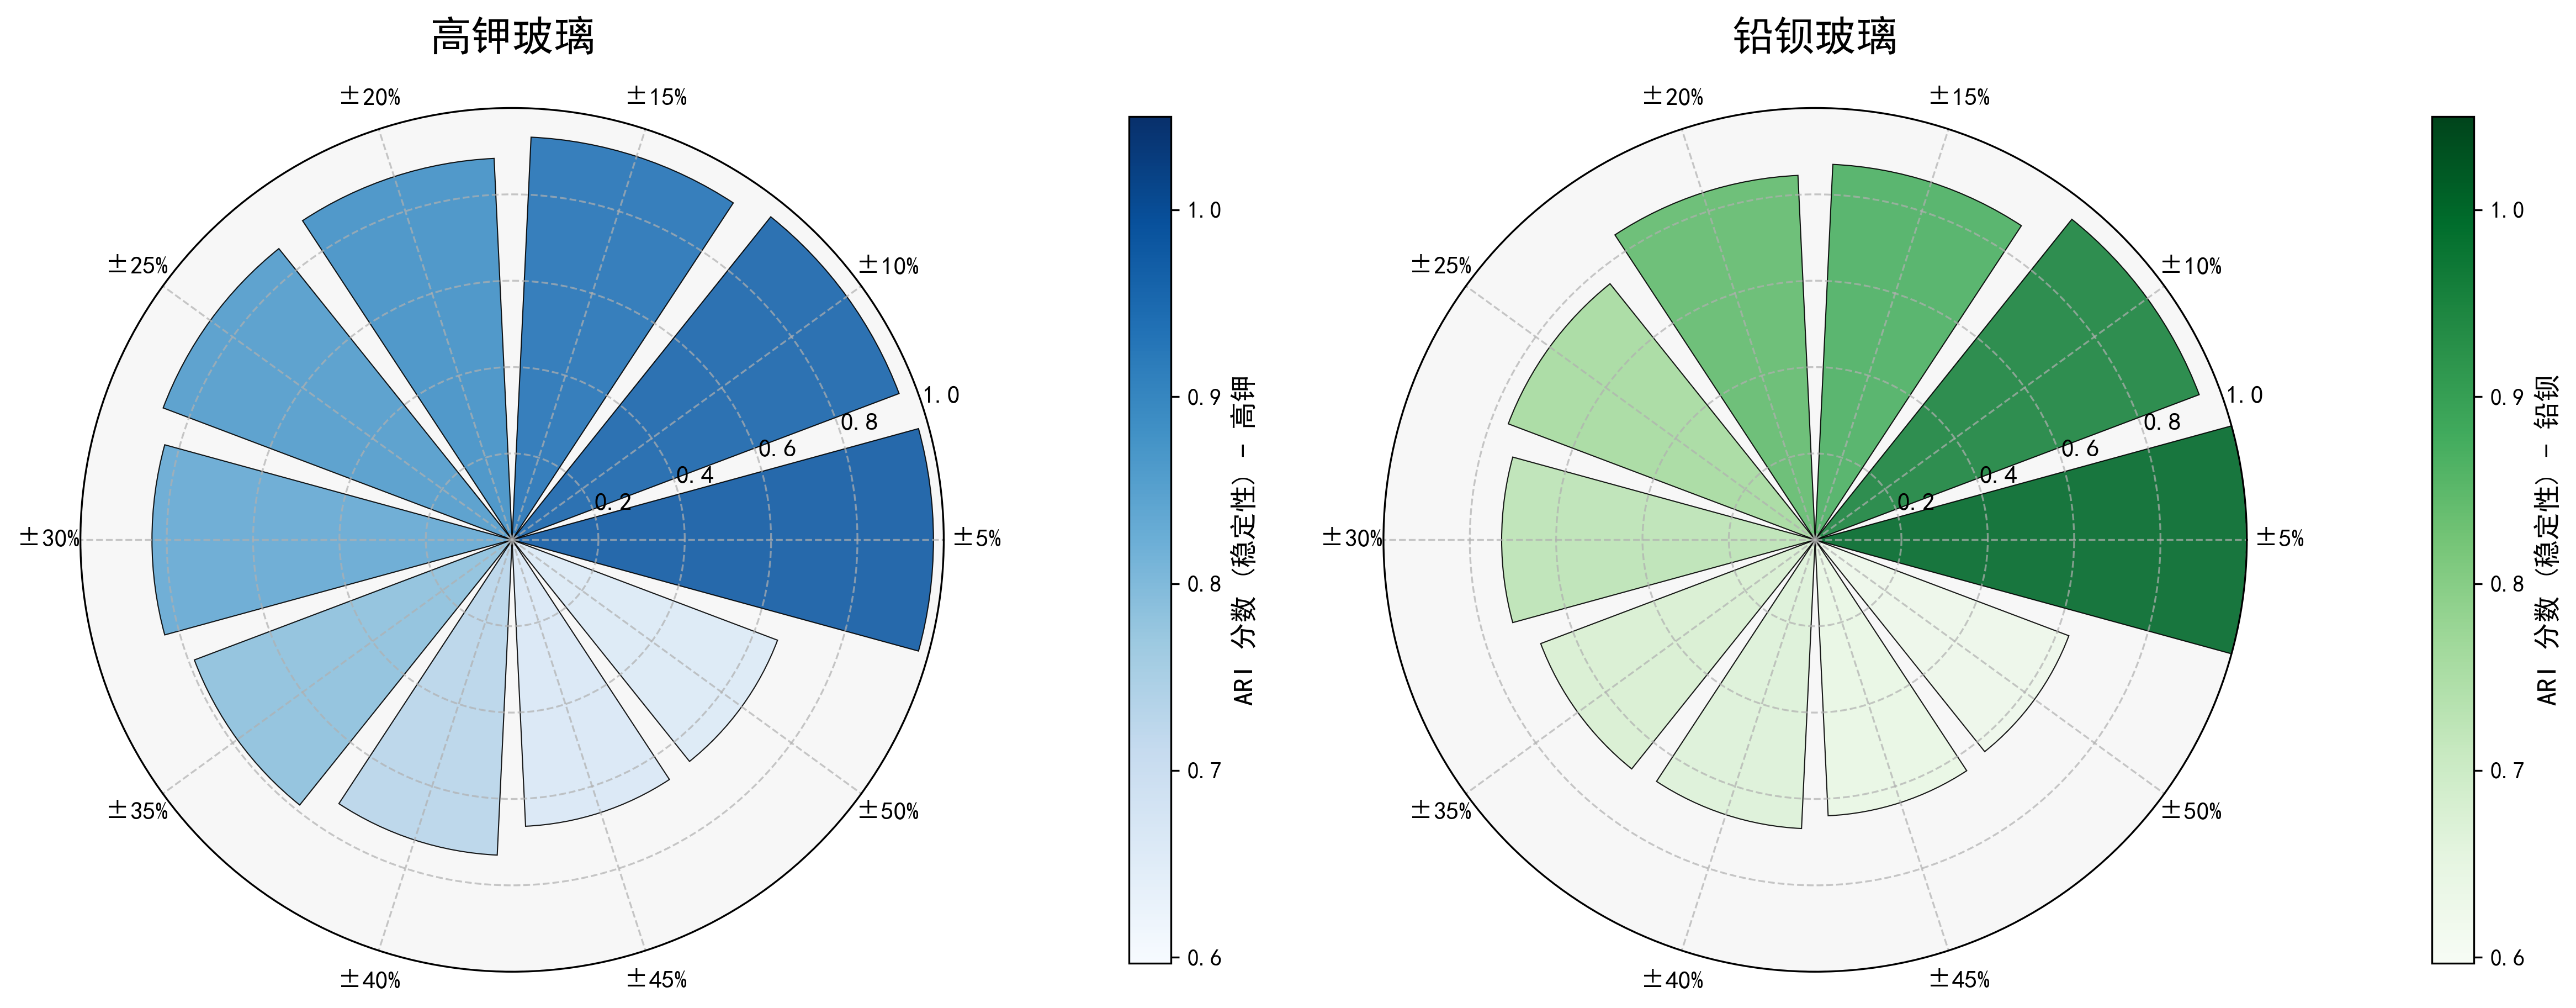
\includegraphics[width=\textwidth]{figs/4问题二/灵敏度分析_玫瑰图_ARI颜色映射.png}
    \caption{不同扰动水平下亚类划分结果的ARI分数}
    \label{fig:ari_sensitivity}
\end{figure}

图\ref{fig:ari_sensitivity}展示了在不同扰动水平下,高钾和铅钡玻璃亚类划分的平均ARI分数。对于高钾玻璃,即使在百分之十的扰动下,平均ARI分数依然高达0.9513。对于铅钡玻璃,在百分之十的扰动下,平均ARI分数为0.9596。在面临潜在的测量误差时,其核心划分依然能够保持高度一致。这证明了我们发现的亚类结构是真实且稳健的,而非随机产生的现象。



\section{问题三:文物类别的鉴别与模型稳健性分析}

本章的核心任务是应用分类模型对未知类别玻璃文物的化学成分进行分析,确定其所属类型,并对分类结果的稳健性与可靠性进行系统性验证。为完成此任务,我们首先进行了一系列对比实验以选择最合适的模型架构,随后采用改进遗传算法对所选模型的超参数进行寻优,构建最终的分类器。最后,我们使用该模型进行预测,并通过双重灵敏度分析来检验结论的稳定性。其整体框架如图\ref{fig:model_framework}所示。

\begin{figure}[H]
    \centering
    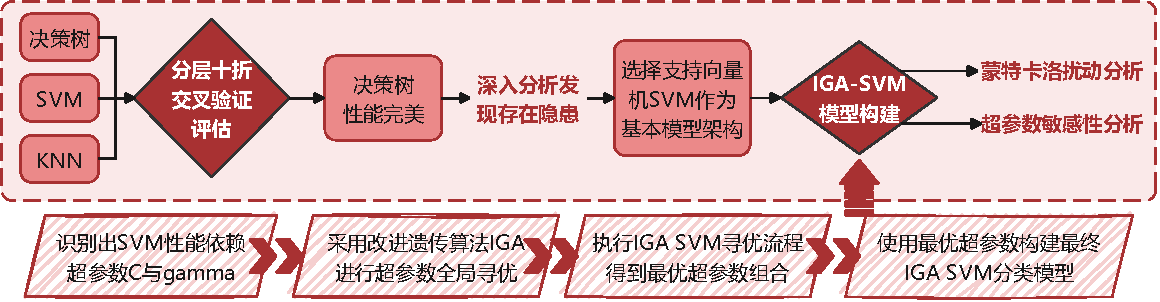
\includegraphics[width=\textwidth]{figs/5问题三/第三问框架.pdf}
    \caption{分类模型框架}
    \label{fig:model_framework}
\end{figure}

\subsection{分类模型的选择与论证}

为建立有效的分类规律,需要从多种候选模型中筛选出最适宜本数据特性的算法。我们选取决策树,K近邻算法以及支持向量机三种具有代表性的模型,在包含全部十四种化学成分及表面风化状况的完整特征集上进行初步性能评估。评估过程采用分层十折交叉验证方法,以保证每次训练与测试中样本类别的分布与原始数据保持一致。各模型的性能指标如表\ref{tab:model_performance}所示。

\begin{table}[H]
    \centering
    \caption{初步模型性能评估}
    \label{tab:model_performance}
    \begin{tabular}{lcc}
        \toprule
        \textbf{模型} & \textbf{准确率} & \textbf{F1分数} \\
        \midrule
        决策树 & 1.0000 & 1.0000 \\
        SVM & 0.9714 & 0.9576 \\
        KNN & 0.9857 & 0.9788 \\
        \bottomrule
    \end{tabular}
\end{table}

评估结果表明,决策树模型在所有性能指标上均达到了1.0的满分。为探究决策树模型取得此结果的原因,我们对其内部结构进行了分析。通过在完整的已分类数据集上训练单个决策树模型,我们发现其特征重要性得分几乎全部集中于氧化铅$PbO$这一项上。模型的可视化结构进一步确认了此发现,如图\ref{fig:decision_tree_structure}所示,该决策树仅在根节点依据氧化铅$PbO$含量是否大于一个特定阈值便完成了对所有样本的分类。

\begin{figure}[H]
    \centering
    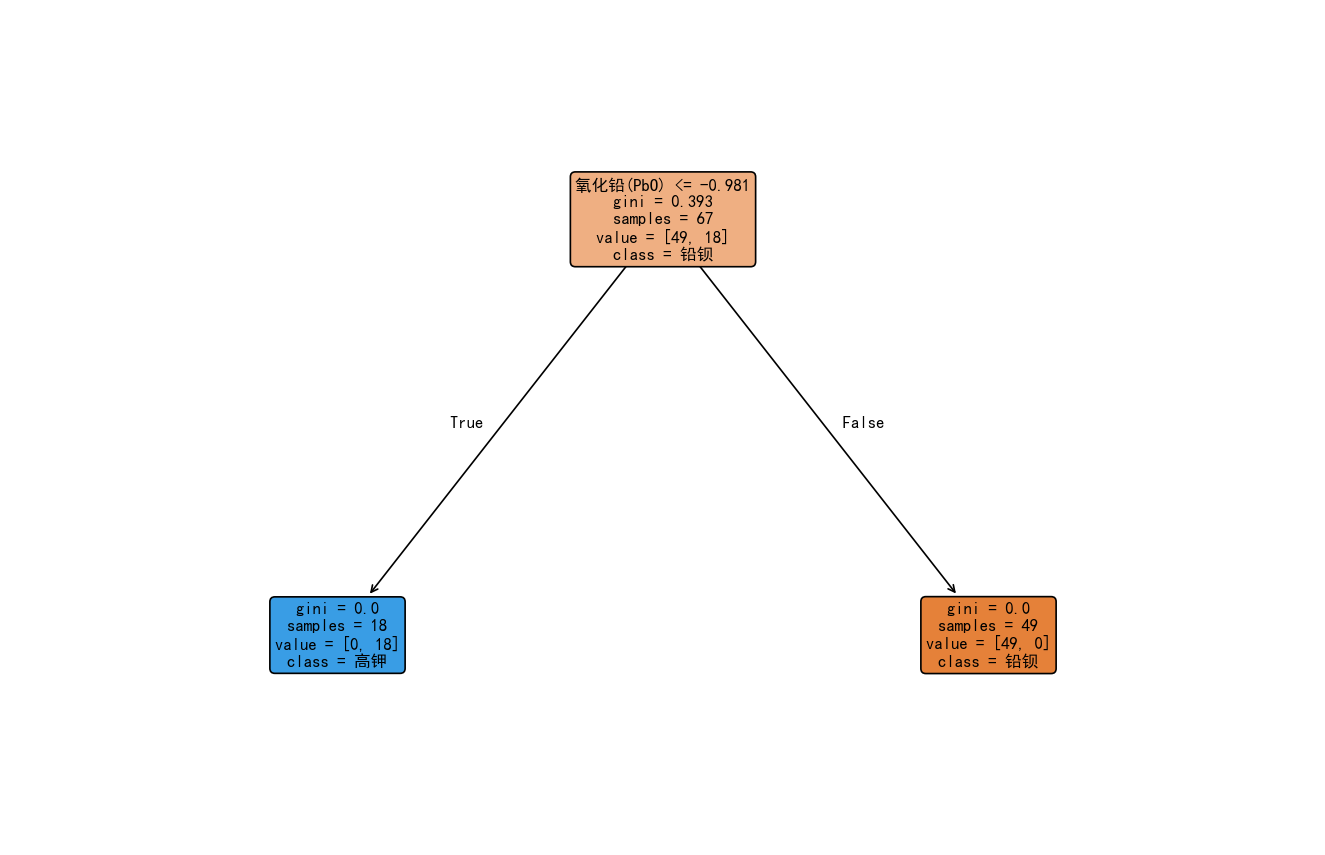
\includegraphics[width=0.8\textwidth]{figs/5问题三/初步决策树可视化图.png}
    \caption{初步决策树模型结构}
    \label{fig:decision_tree_structure}
\end{figure}

尽管决策树表现出很高的评分,但其过分依赖单一特征的决策模式存在稳健性隐患。一个仅凭氧化铅含量进行判断的模型,在面对不含氧化铅但仍属铅钡玻璃体系的未知样本时可能失效,其泛化能力不足。同时,由于该特征的存在,不同模型间的性能差异被掩盖,使得模型对比失去参考价值。基于这些考量,我们排除了将决策树作为最终模型的方案,转而寻求更能利用多维度信息且结构更为稳健的模型。在移除氧化铅特征后进行的补充实验中,支持向量机表现出优越的适应能力,因此我们选择支持向量机作为最终模型的基本架构。

\subsection{基于改进遗传算法的支持向量机模型构建}

支持向量机是一种在高维空间中寻找最优分类超平面的算法,其性能表现高度依赖于正则化系数$C$和核函数系数$\gamma$这两个超参数的设定。为充分发挥支持向量机的性能,我们采用改进遗传算法IGA来代替传统的网格搜索,对其超参数组合进行智能化全局寻优。

支持向量机的基本原理可表述为求解一个软间隔优化问题,其目标函数如下
\begin{equation}
    \min_{\boldsymbol{w}, b, \boldsymbol{\xi}} \frac{1}{2} ||\boldsymbol{w}||^2 + C \sum_{i=1}^{m} \xi_i
\end{equation}
式中$\boldsymbol{w}$与$b$定义了分类超平面,$\xi_i$是允许样本偏离正确边界的松弛变量,而$C$则用以平衡间隔最大化与分类误差。

改进遗传算法IGA是一种模拟生物进化过程的全局优化算法。它将超参数寻优过程转化为一个适者生存的演化过程。算法首先在预设的参数范围内随机生成一个包含多个个体即多组$C$与$\gamma$参数组合的初始种群。随后,算法以分层十折交叉验证的F1分数为适应度函数,对种群中每个个体的优劣进行评估。适应度越高的个体,在后续的遗传操作中被选中作为父代产生后代的概率越大。通过选择,交叉和变异这三种模拟自然繁殖过程的核心算子,算法不断迭代产生适应度更高的新一代种群。此外,精英保留策略确保了每一代的最优个体都能直接进入下一代,保证了寻优过程的收敛性。当达到预设的进化代数或种群适应度不再提升时,算法终止,并输出整个进化过程中适应度最高的个体所对应的超参数组合作为全局最优解。具体机制如\cref{alg:iga_svm}所示。

\begin{algorithm}[H]
    \caption{改进遗传算法IGA优化支持向量机超参数}
    \label{alg:iga_svm}
    \begin{algorithmic}[1]
        \Require
        \Statex 数据集 $D$
        \Statex 种群大小 $N$
        \Statex 最大进化代数 $G_{max}$
        \Statex 交叉概率 $p_c$
        \Statex 变异概率 $p_m$
        \Statex 超参数搜索空间 $S_C, S_{\gamma}$
        
        \Ensure
        \Statex 最优超参数组合 $(C_{best}, \gamma_{best})$

        \Function{IGA-SVM-Optimization}{$D, N, G_{max}, p_c, p_m, S_C, S_{\gamma}$}
            \State 初始化种群 $P_0$:随机生成 $N$ 个个体 $(C_i, \gamma_i)$,其中 $C_i \in S_C, \gamma_i \in S_{\gamma}$
            \State 定义适应度函数 $Fitness(C, \gamma) \leftarrow$ 使用 $(C, \gamma)$ 配置的SVM在数据集$D$上进行分层十折交叉验证的F1分数
            \For{$g = 1$ \textbf{to} $G_{max}$}
                \State 计算当前种群 $P_{g-1}$ 中每个个体的适应度
                \State $P_{new} \leftarrow \emptyset$ \Comment{初始化新一代种群}
                \State 寻找当前种群中的最优个体 $elite \leftarrow \arg\max_{i \in P_{g-1}} Fitness(i)$
                \State $P_{new} \leftarrow P_{new} \cup \{elite\}$ \Comment{精英保留策略}
                
                \For{$k = 1$ \textbf{to} $N-1$}
                    \State \Comment{通过遗传算子生成新个体}
                    \State $parent_1, parent_2 \leftarrow$ \Call{Select}{$P_{g-1}$} \Comment{根据适应度选择父代}
                    \If{$\text{random}(0,1) < p_c$}
                        \State $child \leftarrow$ \Call{Crossover}{$parent_1, parent_2$} \Comment{交叉操作}
                    \Else
                        \State $child \leftarrow parent_1$ \Comment{直接复制}
                    \EndIf
                    
                    \If{$\text{random}(0,1) < p_m$}
                        \State $child \leftarrow$ \Call{Mutate}{$child$} \Comment{变异操作}
                    \EndIf
                    
                    \State $P_{new} \leftarrow P_{new} \cup \{child\}$
                \EndFor
                \State $P_g \leftarrow P_{new}$ \Comment{更新种群}
            \EndFor
            
            \State $(C_{best}, \gamma_{best}) \leftarrow \arg\max_{i \in P_{G_{max}}} Fitness(i)$ \Comment{找出最终的最优个体}
            \State \Return $(C_{best}, \gamma_{best})$
        \EndFunction
    \end{algorithmic}
\end{algorithm}

在具体实现中,我们配置了一个包含15个个体,进化30代的遗传算法。其寻优过程如图\ref{fig:iga_process}所示,该三维瀑布图展示了在迭代过程中,种群的最高适应度,平均适应度与最低适应度的变化情况。图中可见,种群的整体适应度随着进化代数的增加而快速上升并趋于稳定,表明该算法能够高效地在参数空间中搜索到最优解区域。

\begin{figure}[H]
    \centering
    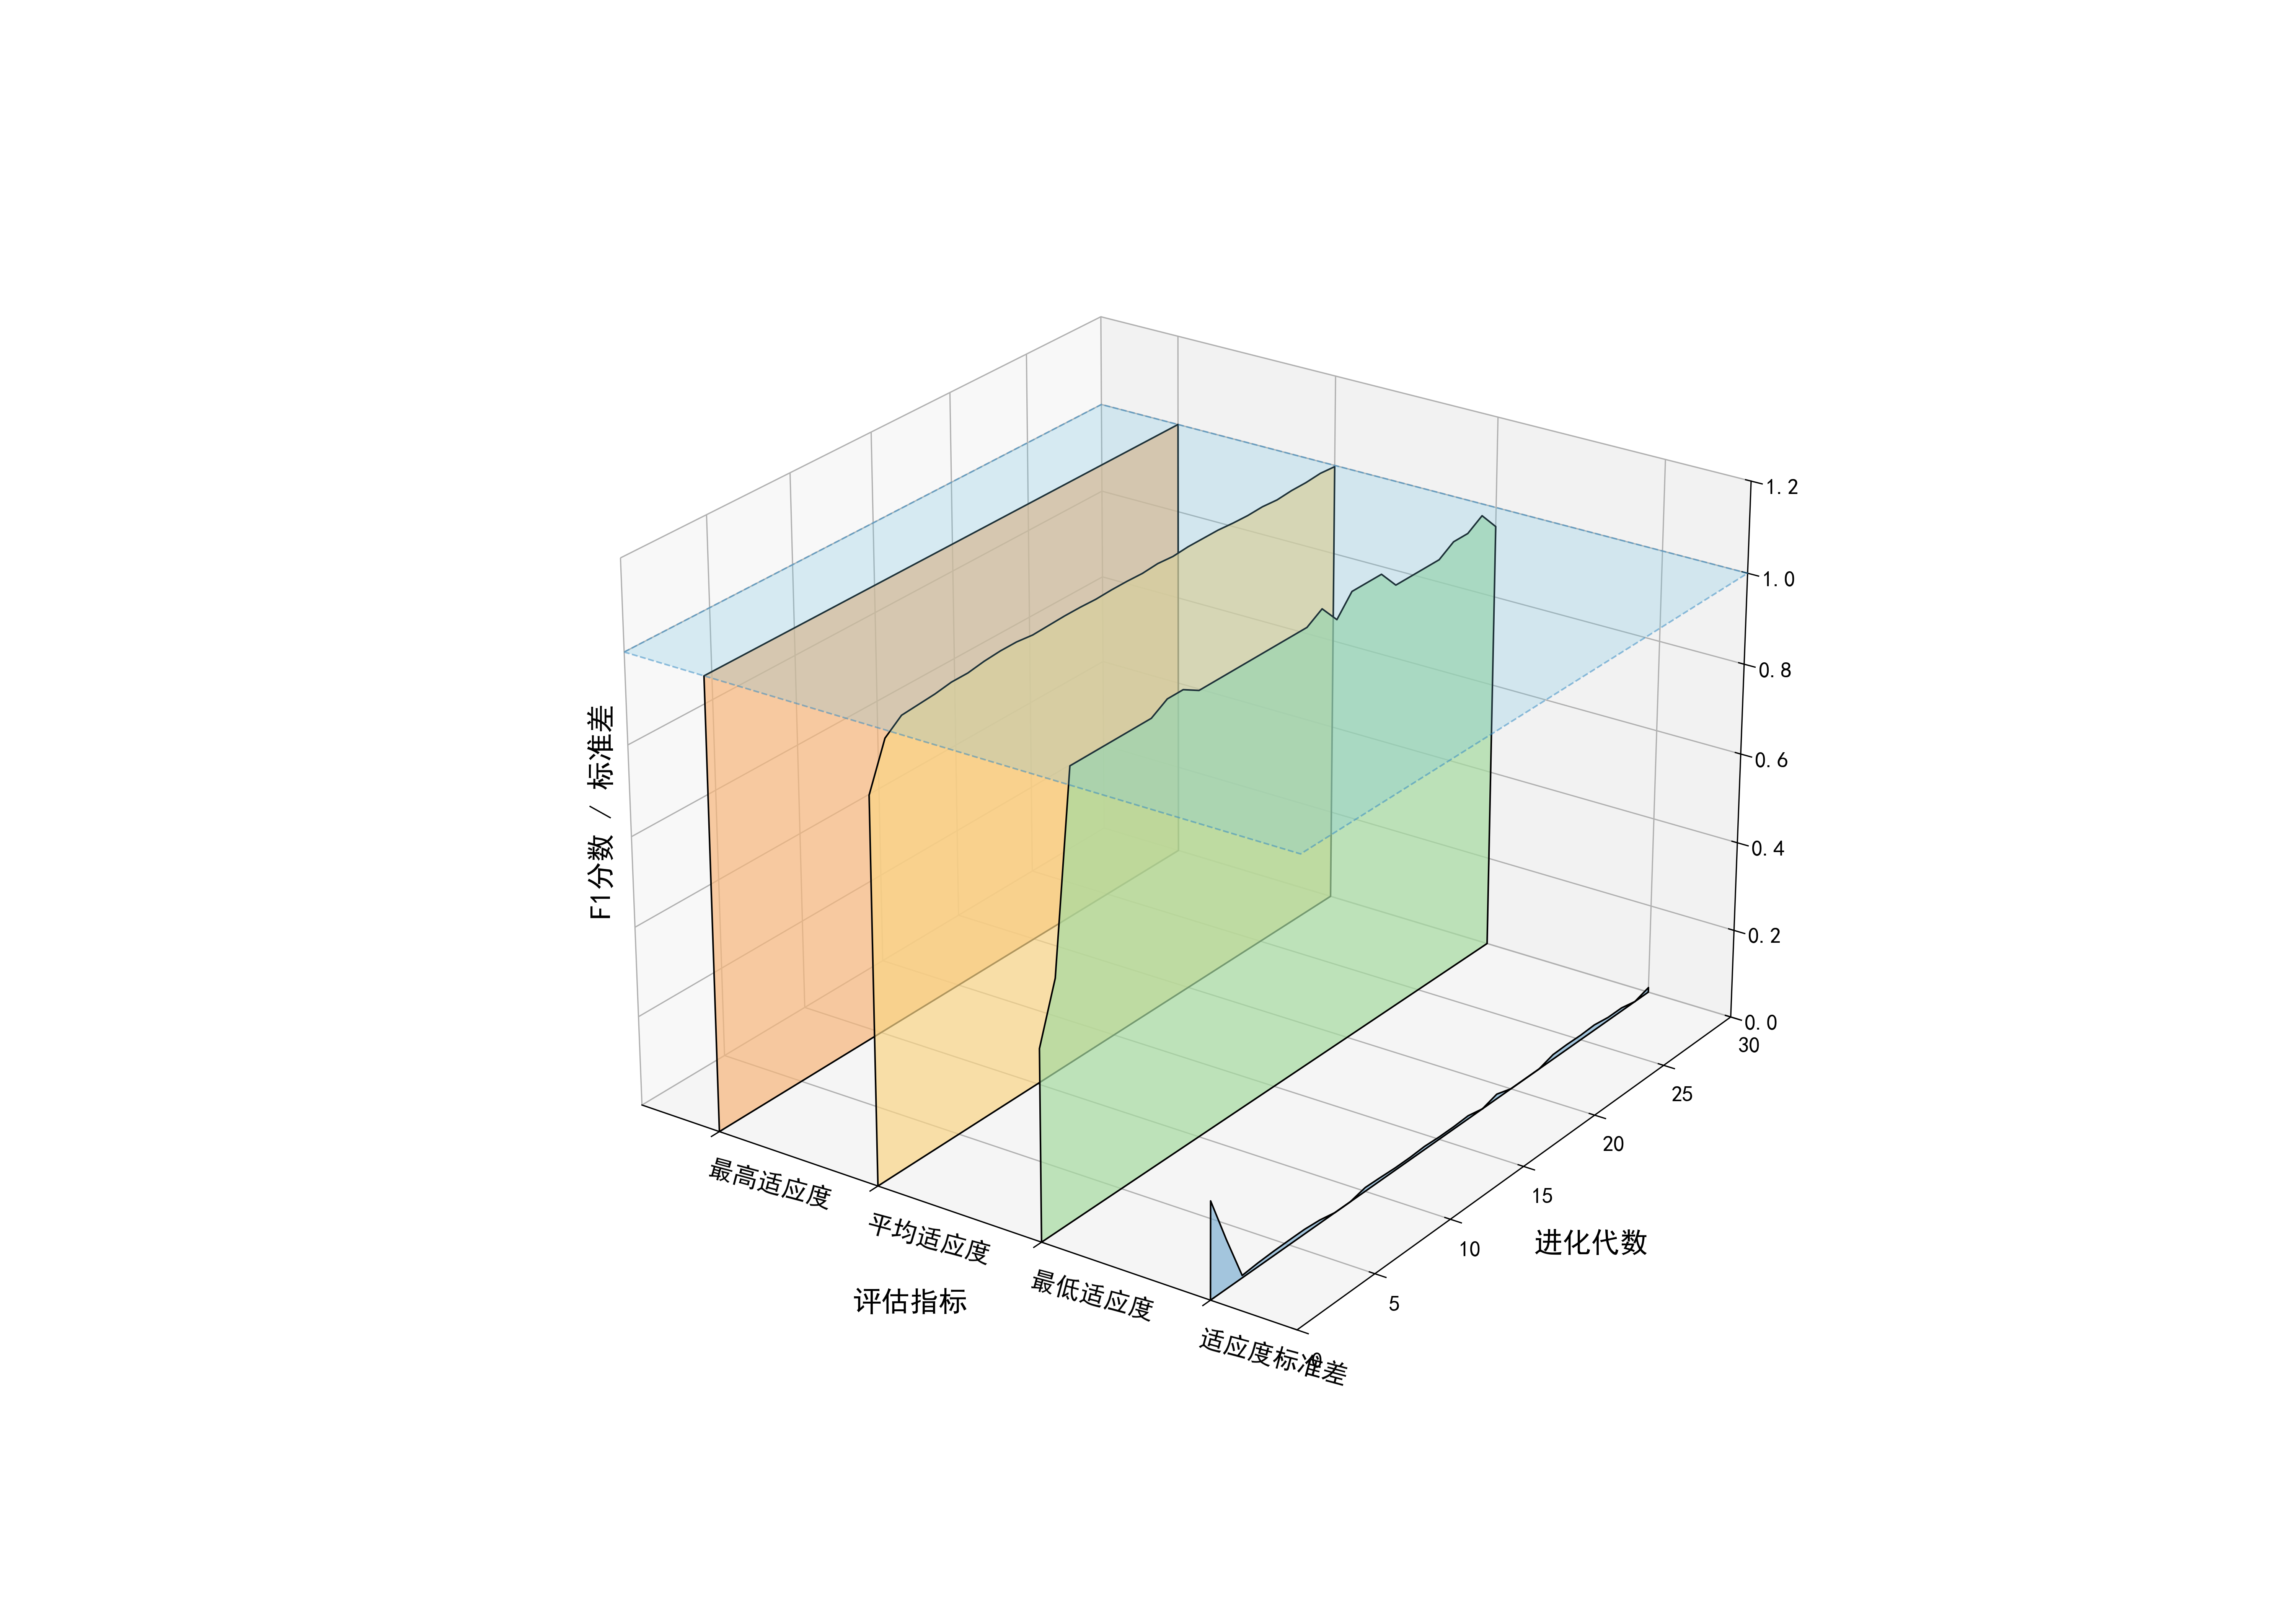
\includegraphics[width=\textwidth]{figs/5问题三/IGA_SVM寻优过程3D瀑布图_最终版.png}
    \caption{改进遗传算法寻优过程}
    \label{fig:iga_process}
\end{figure}

\subsection{最终鉴别结果与双重可靠性验证}

利用前述流程寻得的最优超参数构建最终的IGA-SVM分类模型后,我们将其应用于8个未知类别样本的化学成分数据,完成了最终的类别鉴别。其具体的预测结果如表\ref{tab:prediction_results}所示。

\begin{table}[H]
    \centering
    \caption{未知样本最终预测结果}
    \label{tab:prediction_results}
    \begin{tabular}{|c|c|c|c|c|c|c|c|c|}
        \hline
        \textbf{样本标识} & 0 & 1 & 2 & 3 & 4 & 5 & 6 & 7 \\
        \hline
        \textbf{预测类别} & 高钾 & 铅钡 & 铅钡 & 铅钡 & 铅钡 & 高钾 & 高钾 & 铅钡 \\
        \hline
    \end{tabular}
\end{table}

以确保鉴别结果的可靠性,我们从数据与模型两个维度设计了双重灵敏度分析方案。第一重分析是蒙特卡洛扰动分析,用以检验预测结论对于数据测量误差的稳健性。我们进行了1000次模拟实验,在每次实验中,对样本的部分化学成分数据加入0至5个百分点的随机噪声,然后使用模型重新进行预测。我们通过计算每个样本预测结果在1000次扰动中发生改变的频率,来量化其预测不稳定性。实验结果显示,所有样本的预测不稳定性得分均为0,这表明鉴别结论对于一定范围内的测量误差具有高度的稳定性。

第二重分析是支持向量机超参数敏感性分析,用以检验预测结论对于模型参数选择的稳健性。我们围绕寻得的最优$C$与$\gamma$值构建了一个5乘5的参数网格。对于网格中的每一对参数组合,我们都重新训练支持向量机模型并对未知样本进行预测,然后记录其预测结果与原始最优模型结果不一致的样本数量。分析结果通过热力图进行可视化,如图\ref{fig:svm_sensitivity}所示。

\begin{figure}[H]
    \centering
    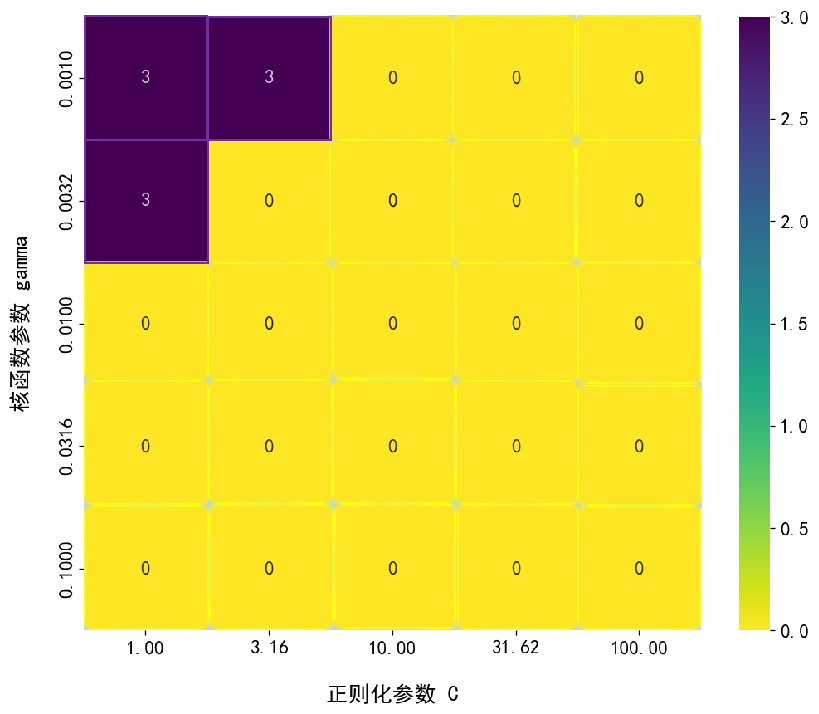
\includegraphics[width=0.7\textwidth]{figs/5问题三/SVM超参数敏感性分析热图.png}
    \caption{支持向量机超参数敏感性分析}
    \label{fig:svm_sensitivity}
\end{figure}

图\ref{fig:svm_sensitivity}中,每个方格的颜色代表在该参数对下预测结果发生改变的样本数量,颜色越深表示变化越大。图中可见,在以最优参数点为中心的广大区域内,颜色均为最浅色,对应数值为0,这意味着预测结果没有发生任何改变。这一广阔的稳定区域证明,最终的鉴别结论对模型超参数的选择不敏感,并非是在某个特定参数点上偶然获得的结果,从而进一步确认了结论的可靠性。

\section{问题四:化学成分关联网络与结构差异分析}

古代玻璃的化学成分体系并非各种元素的随机组合,其背后反映了原料选择与烧制工艺的内在规律。为了探寻不同类别玻璃在配方层面的结构性差异,本章将各类玻璃的化学成分体系构建为网络模型。网络中的节点代表化学成分,节点间的连接则代表成分间在配方中存在的直接关联。通过比较高钾玻璃和铅钡玻璃网络的拓扑结构差异,可以探寻其原料与工艺的深层不同。分析过程始于已分类的化学成分数据,首先应用中心化对数比变换处理成分数据固有的统计约束,随后利用图套索算法计算反映成分间直接关联的偏相关系数并构建网络。进一步理解网络的宏观结构,采用社群发现算法对网络节点进行聚类。最终,所有分析结果被整合至可视化网络图中,以呈现两类玻璃在配方结构上的分别特征。

\subsection{成分数据变换与关联构建方法}

玻璃成分数据属于一种特殊的成分数据,其各组分之和恒定。这一特性会在统计上产生闭合效应,引入虚假的负相关关系。例如,当主要成分二氧化硅$SiO_2$的含量增加时,其他所有成分的相对比例必然下降,即使它们在物理化学上并无关联。直接使用传统相关性分析会产生误导性结论。为解决此问题,本研究引入化学计量学领域处理此类数据的核心技术,即中心化对数比变换。该方法通过对数比值变换,将数据投影到一个无约束的几何空间中,从而消除产生虚假负相关的统计基础,保证后续关联性分析的有效性。

对于一个包含$D$种化学成分的样本向量$\boldsymbol{x} = [x_1, x_2, \dots, x_D]$,首先计算其几何平均数$g(\boldsymbol{x})$。
\begin{equation}
g(\boldsymbol{x}) = \left( \prod_{i=1}^{D} x_i \right)^{1/D}
\end{equation}
随后对每个成分$x_i$进行变换,得到新向量$\boldsymbol{y} = \text{clr}(\boldsymbol{x})$的第$i$个元素$y_i$。
\begin{equation}
y_i = \ln\left(\frac{x_i}{g(\boldsymbol{x})}\right)
\end{equation}
在具体计算中,数据中的零值被一个极小的正数替代,以确保对数运算的有效性。

在变换后的数据基础上,需要探寻成分间排除了所有其他成分影响后的直接关联。常规相关系数无法区分直接关系与间接关系,因此需要计算偏相关系数。图套索算法是估计偏相关网络的常用方法,它通过求解一个带$L1$惩罚的优化问题,从数据中估计出一个稀疏的逆协方差矩阵,即精度矩阵,并由此推导出偏相关关系。其目标函数如下。
\begin{equation}
\hat{\Theta} = \arg\max_{\Theta \succ 0} \left( \log(\det\Theta) - \text{tr}(S\Theta) - \lambda \|\Theta\|_1 \right)
\end{equation}
其中,$S$是变换后数据的样本协方差矩阵,$\lambda$是控制稀疏度的正则化参数,$L1$惩罚项会使精度矩阵$\Theta$中许多不重要的元素变为零。得到$\Theta$后,任意两个变量$i$和$j$之间的偏相关系数$\rho_{ij \cdot \text{rest}}$可由以下公式算出。
\begin{equation}
\rho_{ij \cdot \text{rest}} = - \frac{\Theta_{ij}}{\sqrt{\Theta_{ii} \Theta_{jj}}}
\end{equation}
当且仅当$\Theta_{ij}$不等于零时,变量$i$和$j$之间存在直接关联。为避免人工设定正则化参数的主观性,本研究采用交叉验证版本的方法,使其能够自动为不同数据集找到最优的正则化参数。

\subsection{网络社群结构发现}
充满连接的网络图虽然信息量大,但难以直接观察其核心结构。为从更高维度分析网络,本研究引入社群发现算法,其作用是自动识别网络中的模块或社群。一个社群是内部连接远比外部连接紧密的节点集群,在当前背景下可能代表了一组在化学功能或来源上高度相关的成分。本研究选用鲁汶算法,它通过优化模块度指标来迭代地寻找网络的最优社群划分。

\begin{algorithm}[htbp]
	\caption{鲁汶社群发现算法}
	\label{alg:louvain}
	\begin{algorithmic}[1]
		\Require
		\Statex 带权重的图 $G = (V, E, w)$
		\Ensure
		\Statex 节点的社群划分 $P$

		\State 初始化:对于所有节点 $v \in V$,将其分配至独立的社群 $C_v \leftarrow \{v\}$
		\Repeat
			\State 设置标记 $improved \leftarrow \text{false}$
			\State \Comment{第一阶段:节点移动}
			\Repeat
				\State 设置标记 $moved \leftarrow \text{false}$
				\For{每一个节点 $v \in V$}
					\State $C_{current} \leftarrow$ 节点 $v$ 当前所在的社群
					\State $\Delta Q_{max} \leftarrow 0$
					\State $C_{best} \leftarrow C_{current}$
					\For{节点 $v$ 的每一个邻居 $u$}
						\State $C_{neighbor} \leftarrow$ 节点 $u$ 所在的社群
						\If{$C_{neighbor} \neq C_{current}$}
							\State 计算将节点 $v$ 从 $C_{current}$ 移至 $C_{neighbor}$ 的模块度增益 $\Delta Q$
							\If{$\Delta Q > \Delta Q_{max}$}
								\State $\Delta Q_{max} \leftarrow \Delta Q$
								\State $C_{best} \leftarrow C_{neighbor}$
							\EndIf
						\EndIf
					\EndFor
					\If{$C_{best} \neq C_{current}$}
						\State 将节点 $v$ 从 $C_{current}$ 移至 $C_{best}$
						\State $moved \leftarrow \text{true}$
						\State $improved \leftarrow \text{true}$
					\EndIf
				\EndFor
			\Until{$moved = \text{false}$}
			\State \Comment{第二阶段:网络聚合}
			\If{$improved = \text{true}$}
				\State $V' \leftarrow \emptyset$, $E' \leftarrow \emptyset$
				\State 将当前划分中的每个社群 $C$ 视为一个新的超级节点
				\State $V' \leftarrow$ 所有超级节点的集合
				\State 根据原始社群间的连接权重之和,计算超级节点间的边和权重,得到 $E'$
				\State 构建新的聚合图 $G \leftarrow (V', E')$
			\EndIf
		\Until{$improved = \text{false}$}
		\State \Return 当前图 $G$ 中节点的最终社群划分 $P$
	\end{algorithmic}
\end{algorithm}


鲁汶算法是一个多层次的迭代过程。第一阶段为节点移动,初始时每个节点是独立的社群,算法遍历所有节点,尝试将每个节点移动到其邻居所在的社群中,并计算此举带来的模块度增益,节点最终被分配到能使其模块度增益最大的邻居社群中。此过程反复进行,直到没有节点移动能再提升模块度。第二阶段为网络聚合,将第一阶段形成的每个社群压缩成一个超级节点,构建一个新的聚合网络,社群间的连接权重等于原始节点间连接权重的总和。算法重复这两个阶段,直到网络的模块度不再有显著提升,从而得到一个层次化的社群结构。该算法的具体步骤如算法\ref{alg:louvain}所示。


\subsection{两类玻璃化学成分关联网络分析}
最终的关联网络可视化图整合了偏相关强度,社群归属和节点重要性等多个维度的分析结果。图中每个节点代表一种化学成分,节点大小由连接数量与连接强度共同决定,连接广泛且作用强度高的成分由此成为网络的核心枢纽。节点颜色对应其所属的结构社群,颜色相同的节点在配方体系中构成一个功能或来源上相互关联的模块。节点间的连接代表成分间排除了其他变量影响后的直接关联,连接粗细正比于偏相关系数的绝对值,用以表现关联的强度,橙色连接为正相关,青色连接为负相关。

\begin{figure}[htbp]
    \centering
    \begin{minipage}[b]{0.48\textwidth}
        \centering
        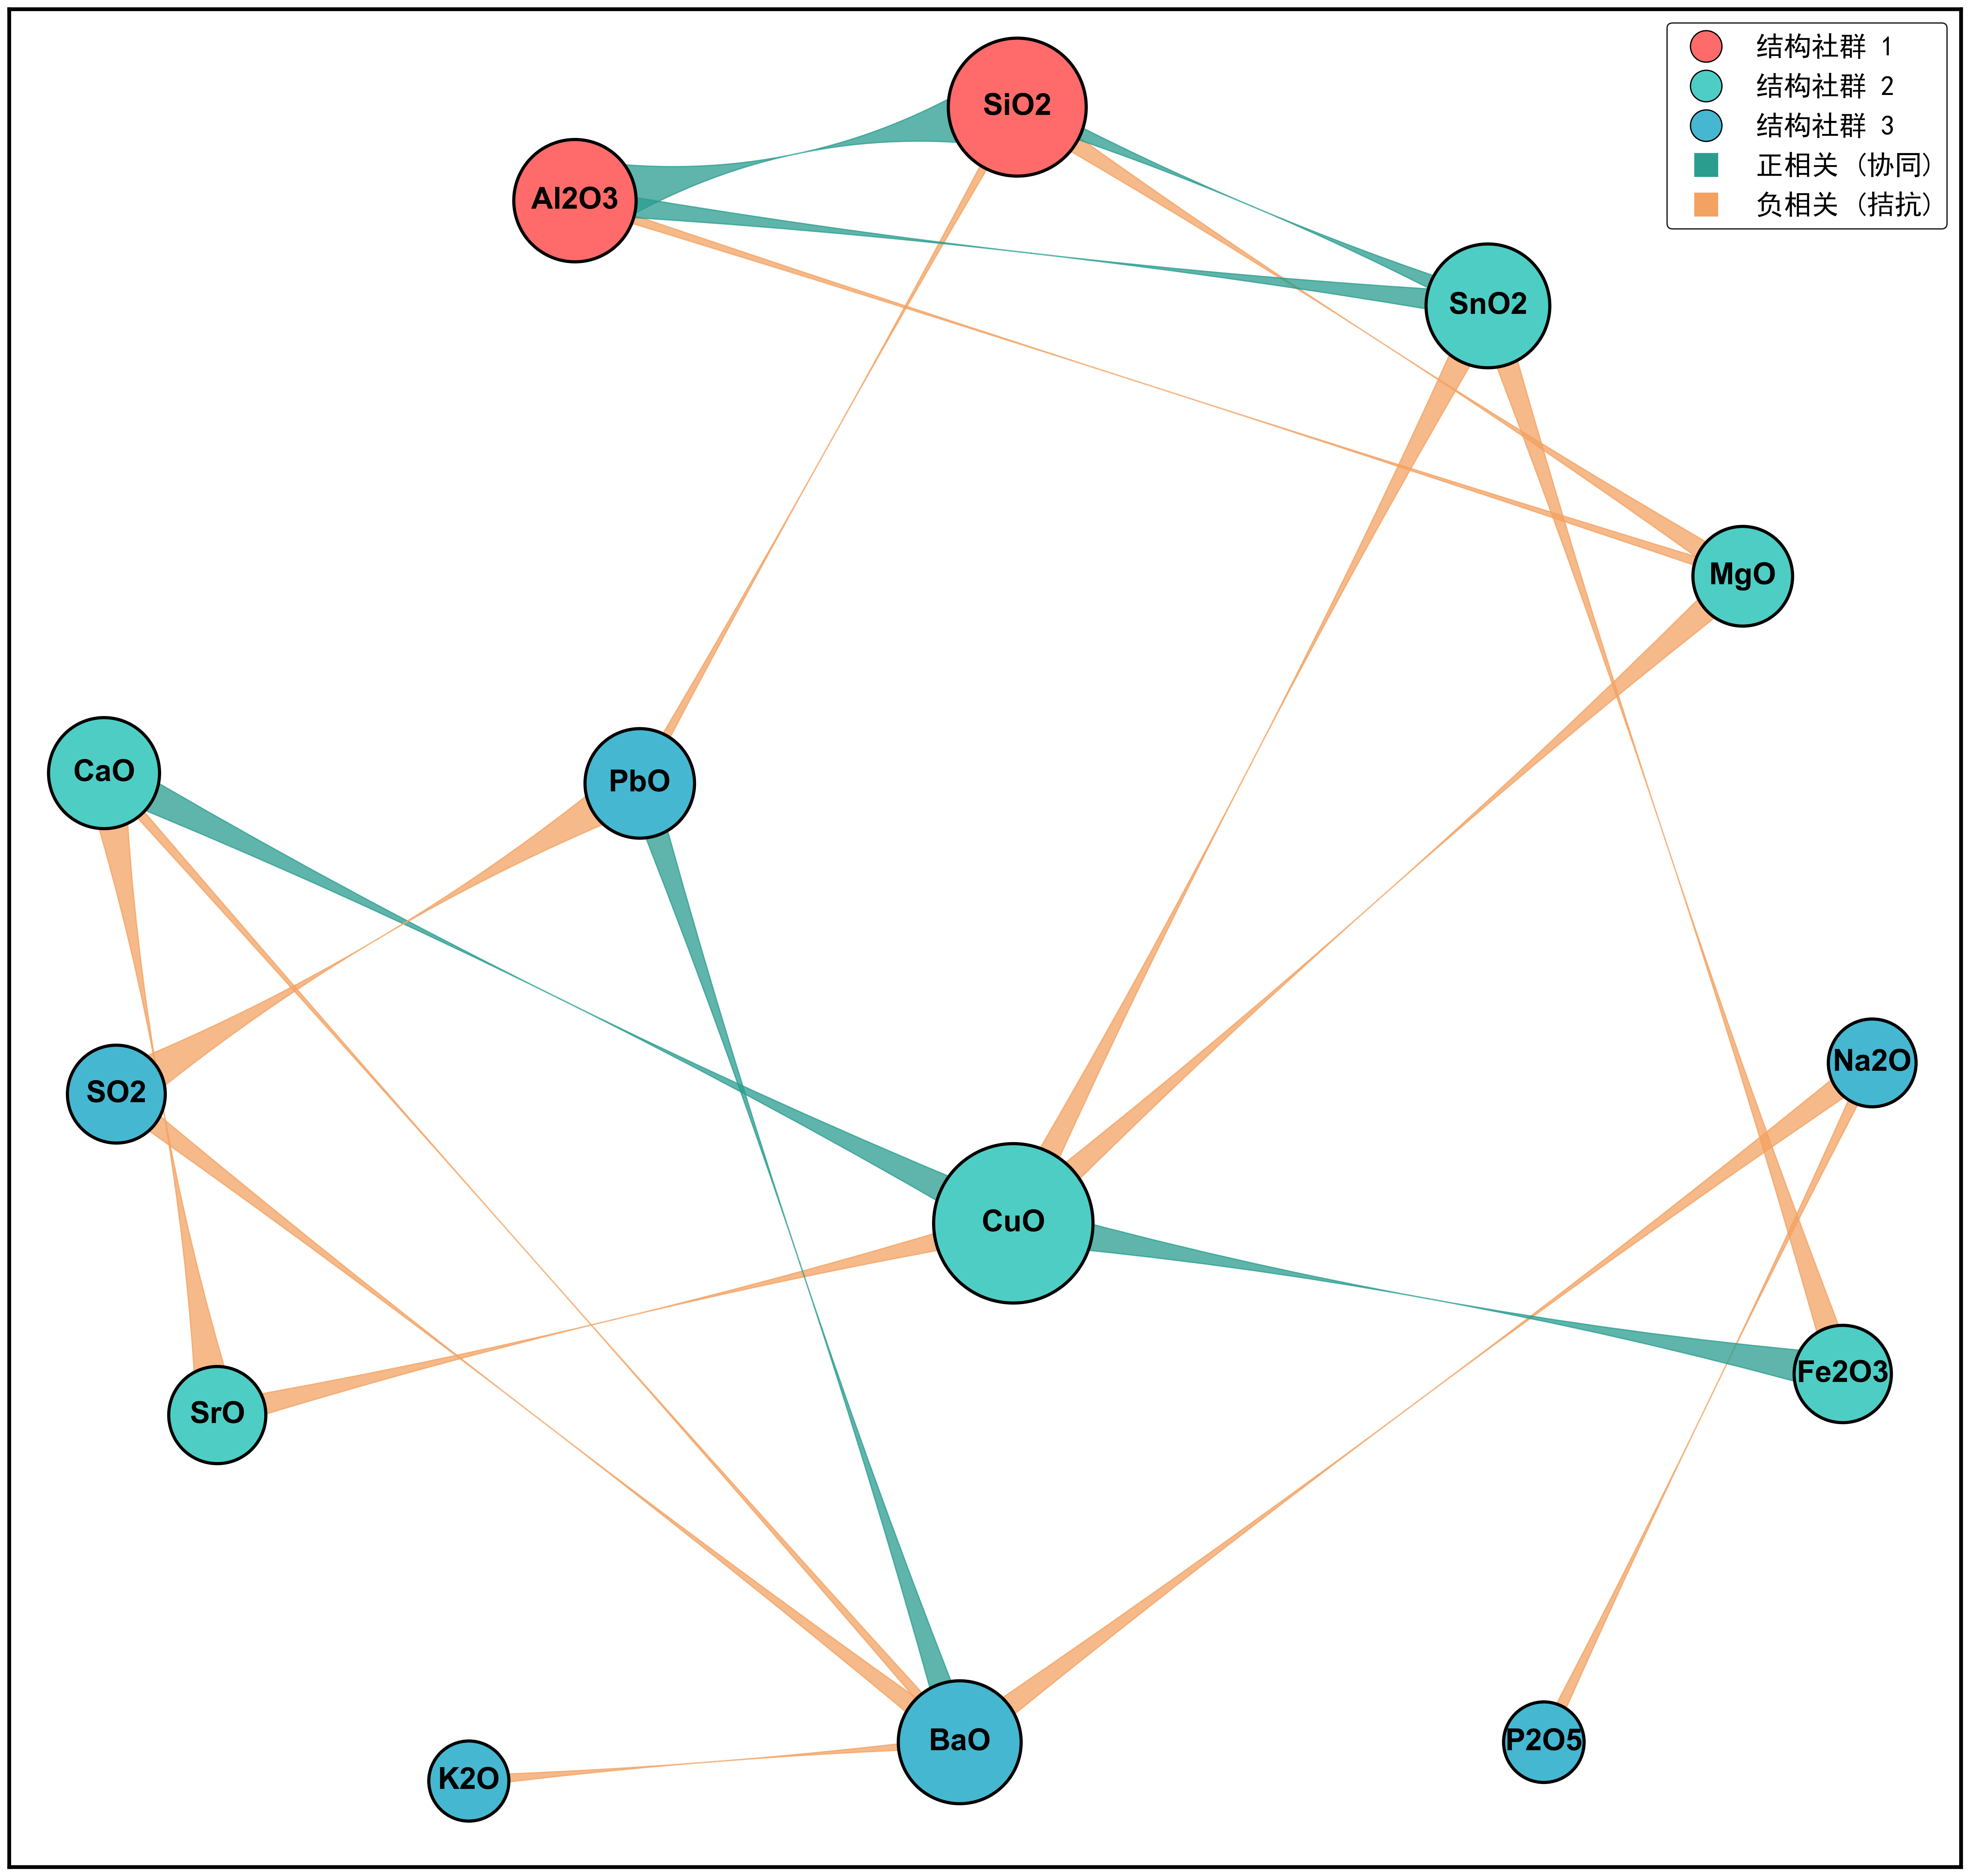
\includegraphics[width=\textwidth]{figs/6问题四/高钾_Network_Final_Soft_Bright.png}
        \caption*{高钾玻璃化学成分关联网络}
    \end{minipage}
    \hfill
    \begin{minipage}[b]{0.48\textwidth}
        \centering
        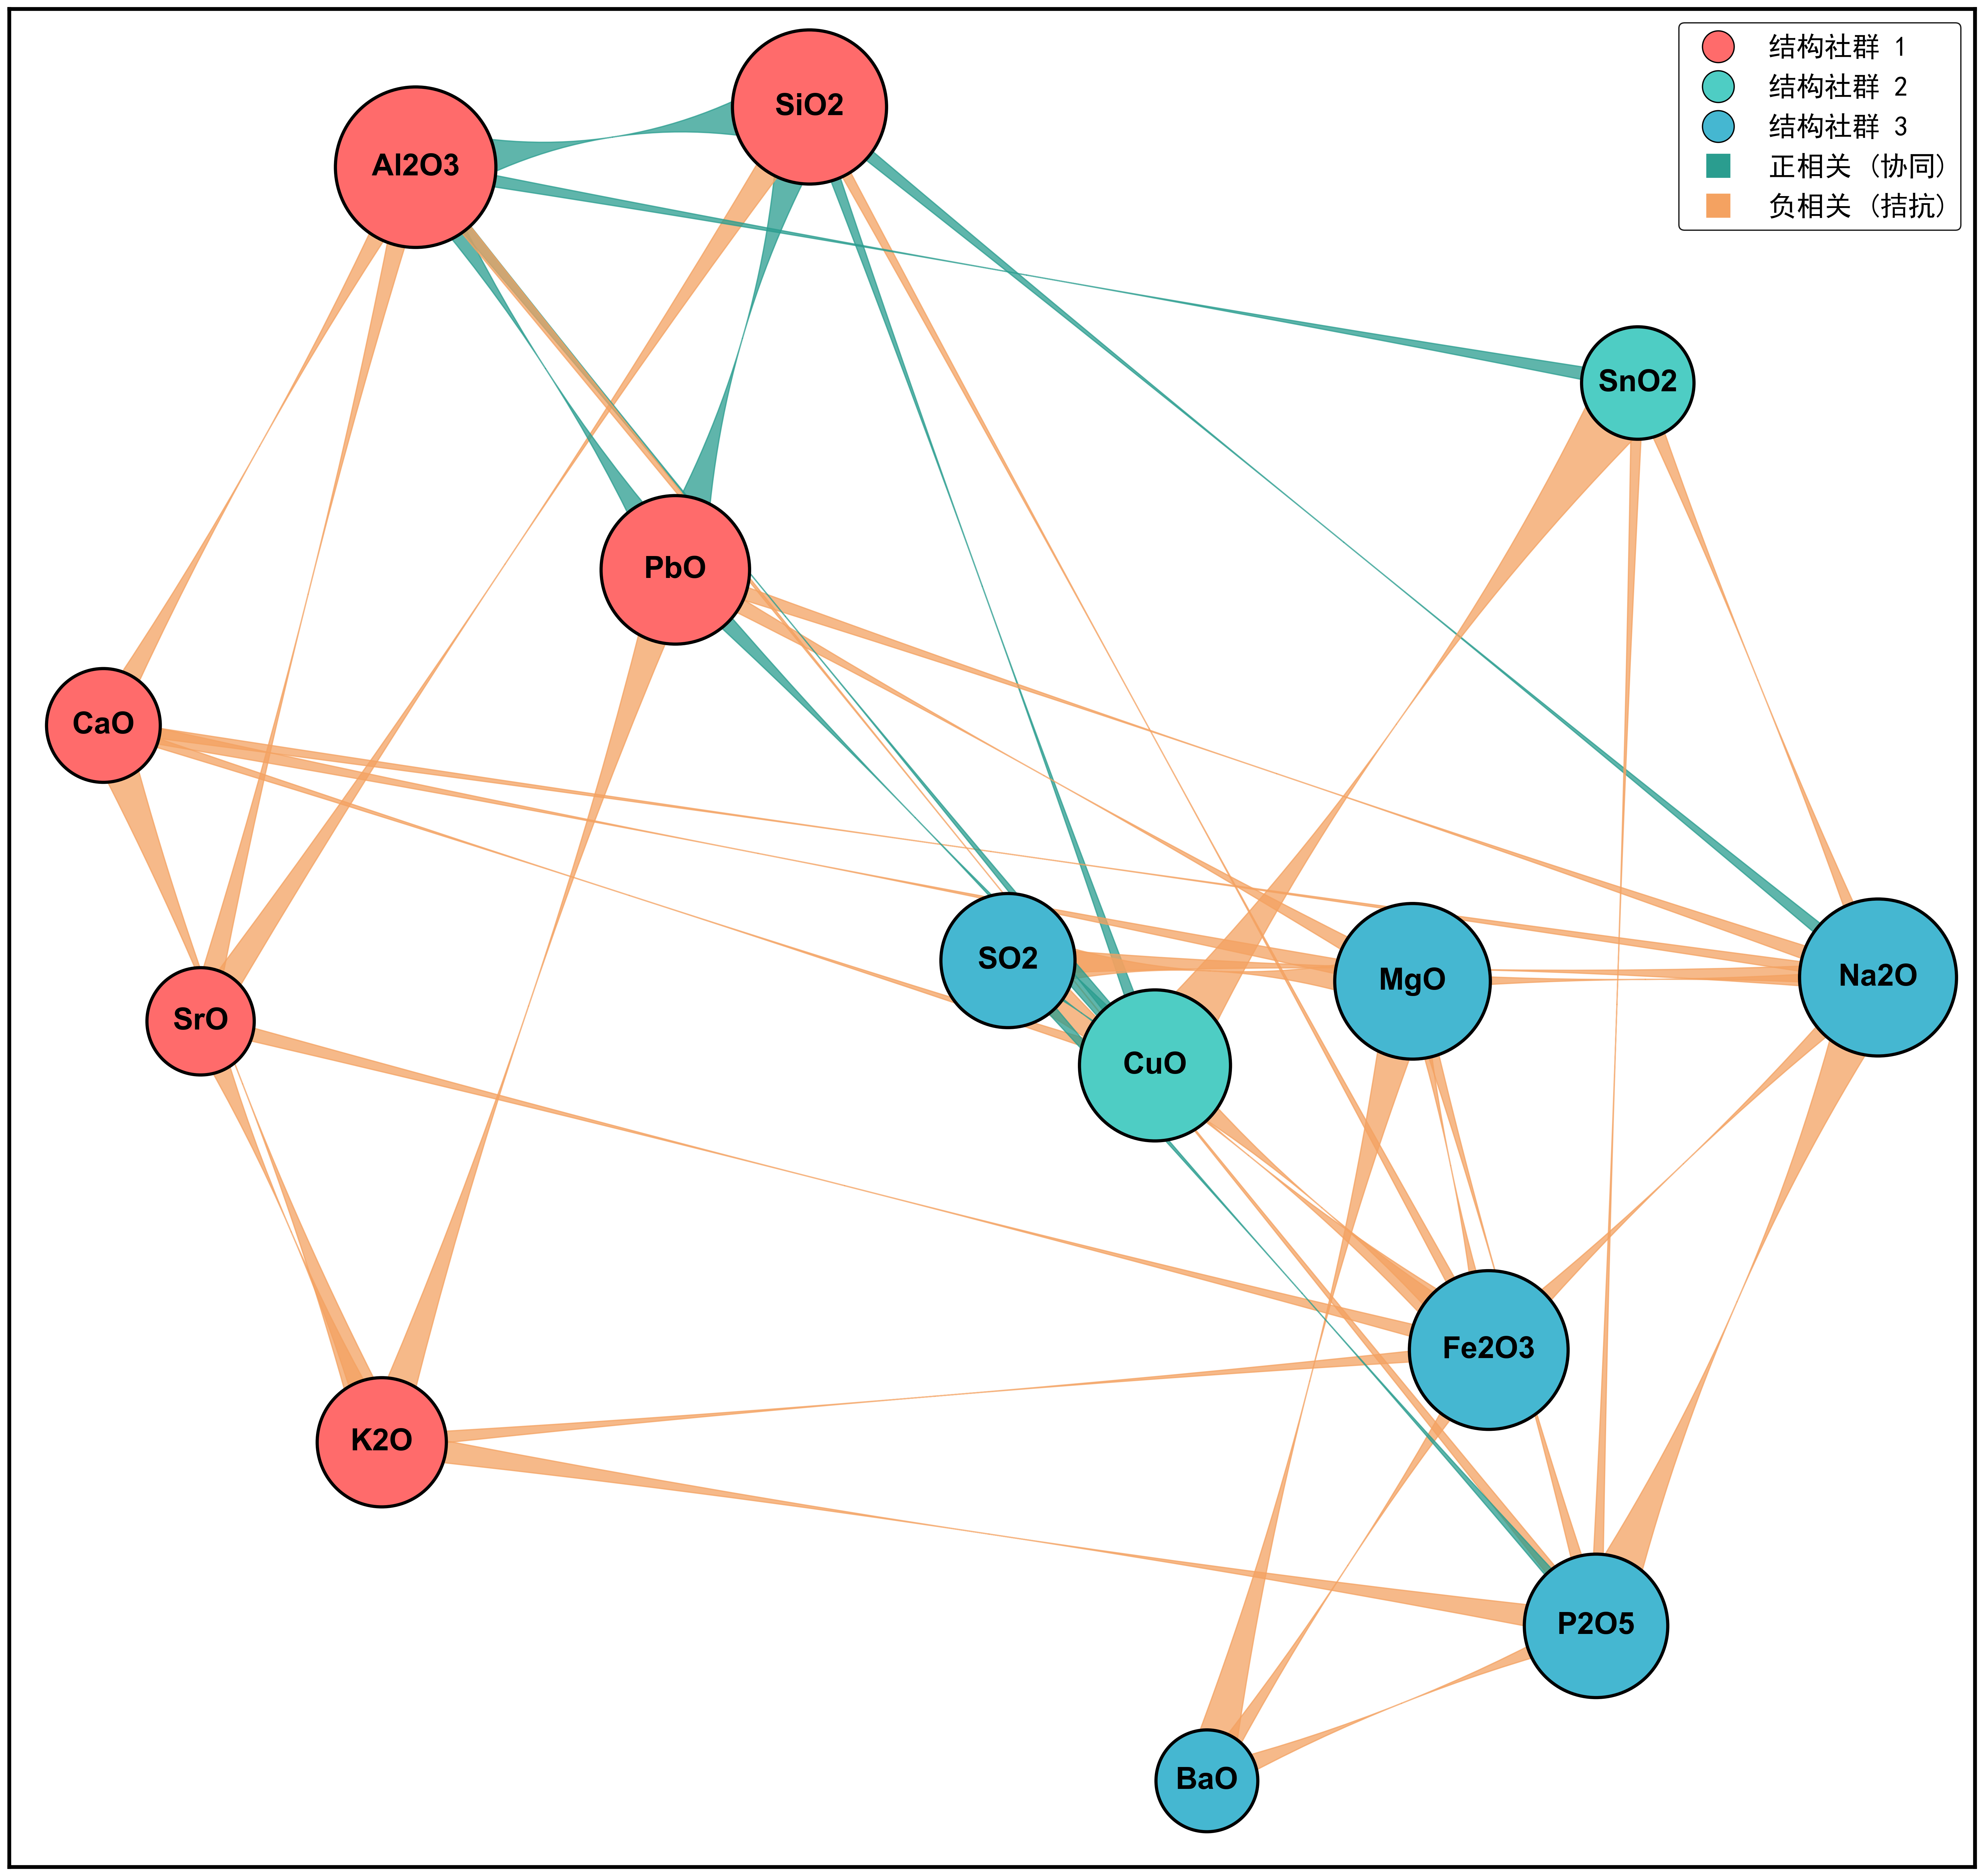
\includegraphics[width=\textwidth]{figs/6问题四/铅钡_Network_Final_Soft_Bright.png}
        \caption*{铅钡玻璃化学成分关联网络}
    \end{minipage}
    \caption{两类玻璃化学成分关联网络对比}
    \label{fig:networks}
\end{figure}

图\ref{fig:networks}A展示了高钾玻璃的化学成分关联网络。其网络结构呈现两个主要社群。社群一为红色,由玻璃主干成分二氧化硅$SiO_2$和氧化铝$Al_2O_3$构成。社群二为青色,包含了氧化铜$CuO$和氧化钡$BaO$在内的多种金属氧化物。一个值得注意的现象是,作为高钾玻璃标志性成分的氧化钾$K_2O$并未归入任何主要社群,这表明在排除了其他成分的普遍影响后,它与其他成分的直接关联不集中。网络中,氧化铜$CuO$,氧化钡$BaO$和二氧化硅$SiO_2$的节点尺寸较大,是网络中的关键节点。从关联上看,二氧化硅$SiO_2$与氧化铅$PbO$之间存在负相关,而氧化铜$CuO$与氧化钡$BaO$之间也表现出负相关关系。

图\ref{fig:networks}B展示了铅钡玻璃的化学成分关联网络。该网络在结构上与高钾玻璃存在显著差异,共形成了三个社群。社群一为红色,是网络的主体,它同时包含了作为玻璃骨架的二氧化硅$SiO_2$和作为助熔剂的氧化铅$PbO$与氧化钾$K_2O$,说明这些成分在配方中协同作用。社群二为青色,主要由氧化钡$BaO$和氧化铁$Fe_2O_3$等成分组成。社群三为蓝色,由氧化锡$SnO_2$和氧化钠$Na_2O$构成。网络的核心节点是氧化铅$PbO$,二氧化硅$SiO_2$和氧化铝$Al_2O_3$。网络中最突出的关联是氧化铅$PbO$与二氧化硅$SiO_2$之间强度很高的正相关,这表明两者在铅钡玻璃的形成过程中有相互促进的作用。与此相对,氧化铝$Al_2O_3$与二氧化硅$SiO_2$之间存在强度较高的负相关。两类玻璃关联网络在社群构成与核心关联上的不同,系统地反映了它们在原料选择与烧制工艺上的区别。




\newpage

% 参考文献
\bibliographystyle{plain}
\bibliography{reference}

\newpage

\end{document}